\chapter{The Concepts of Quantum Mechanics}
\label{chap01}

\section{Introduction}

It is assumed that all students reading this material have had some 
course (e.g., the traditional semester of a junior-level physical 
chemistry course) presenting the basic elements of quantum mechanics 
with some treatment of the hydrogen atom, the harmonic oscillator, 
and angular momentum.  This course will concentrate on the 
explanation of the structure and reactivity of molecules using 
quantum mechanical ideas.  The explanations will stress qualitative 
and semi-quantitative considerations with the emphasis on developing 
\emph{principles} (based on quantum mechanics) that can be used to make 
reliable \emph{predictions on new systems} (rather than merely 
rationalize known results).

This chapter is a review of materials that all students should have
had previously, but with an emphasis on those points that will be
important later in the course.

The basic principles of quantum mechanics are summarized in Section 1.
A key idea here is that \emph{in the classical description of an atom,
  the electron would collapse into the nucleus}.  The critical
difference with the quantum description is that the kinetic energyis
proportional to the averge value of the square of the gradient of the
wavefunction, $T = 1/2 \langle | \nabla \varphi |^2\rangle$.
Consequently, for an electron sitting on the nucleus, the knetic
energy is infinite (since $\nabla \varphi$ is infinite).  This forces
the electron to remain distributed over a \emph{finite} region
surrounding the nucleus and prevents the collapse of the electron into
the nucleus.  Thus, \emph{the quantum description is essential for
  stability of atoms}.  We will find in later chapters that
modifications in the kinetic energy (due to superposition of orbitals)
also plays the key role in the formation of chemical bonds.

Throughout this course we will be searching for qualitative ideas 
concerning the sizes and shapes of wavefunctions and for simple ways 
of predicting the energy ordering of the states of a system.  A useful 
concept here is the \emph{nodal} theorem described in Section 0.3.  
Basically, this theorem tells us that the grund state of a system is 
everywhere positive [no nodal planes (zeros) interior to the boundaries 
of the system].

\section{Basic Principles of Quantum Mechanics}
    
In this section, we highlight the basic concepts of quantum mechanics
relevant to this course. All of these ideas should be familiar to you; 
good references for reviewing these topics and for outside reading 
during the first part of Ch 120a are given in references
\cite{levineqm} and \cite{eyringqm}.

\subsection{The Need for Quantum Mechanics}
    
In order to see why quantum mechanics is so important to chemistry, let us 
examine the classical mechanical description of the hydrogen atom

The total energy is given by E = T + V where the kinetic energy is
\begin{equation}
T = {1 \over 2} mv^2 - {1 \over 2m} p^2
\label{eqno1-1}
\end{equation}
where $m$, $v$, and $p$ are the mass, velocity, and momentum of the electron,
and the potential energy is
\begin{equation}
V = {q_pq_e \over r} = - {e^2 \over r}
\end{equation}
where $q_e = -e$ and $q_p = +e$, and the charge of the electron and 
proton, and $r$ is the distance between them.  
    
Actually, the total kinetic energy of the hydrogen atom has two terms,
\begin{equation}
T = {1 \over 2} m_p v_p^2 + {1 \over 2} m_e v_e^2 = {1 \over 2m_p} \left( 
p_p \right)^2 + {1 \over 2m_e} \left( p_e \right)^2.
\label{eqno1-2}
\end{equation}
However, considering the case where there is no net motion (i.e., no net 
inertia or momentum) leads to $p_p + p_e = 0$ and hence, $(p_p)^2 = 
(p_e)^2$, so that equation (\ref{eqno1-2}) becomes
\begin{equation}
T = {1 \over 2 \mu} \left( p_e \right)^2,
\end{equation}
where
\begin{equation}
{1 \over \mu} = {1 \over m_p} + {1 \over m_e}
\end{equation}
or
\begin{equation}
\mu = {m_p m_e \over m_p + m_e} = {m_e \over 1 + {m_e \over m_p}}.
\end{equation}
Since $m_p = 1836 m_e$, then $\mu = 0.9995 m_e$, and for our purposes 
we can consider just the kinetic energy of the electron as in 
equation (\ref{eqno1-1}).
    
The ground state is when the system has its lowest possible total energy.
Any other state, higher energy, is referred to as an excited state.  Generally, 
systems in excited states will eventually decay to lower energy states, and
we will be interested in the stable, ground, states.  For system containing 
charges, this is accompanied by emission of light. The lowest kinetic energy 
occurs for $p = 0$, leading to $T = 0$, while the lowest potential energy 
occurs for $r = 0$, leading to $V = -\infty$. Thus, in the
classical description, the ground state of the hydrogen atom has the 
electron standing, or sitting, on the nucleus, leading to $E = 
- \infty$. Since the charges cancel and the atom has a
radius of zero, these atoms would not combine to form molecules. Thus, in
classical mechancis the atom is not stable!  If classical mechanics 
provided the proper description of atoms, we would not be here pondering 
the  universe.

The solution of this problem is provided in quantum mechanics, as will be 
discussed.  Essentially, the conclusion is that electrons must be described 
in terms of wavefunctions $\Psi({\bf r})$, where the shape of the 
wavefunction simultaneously determines both the kinetic energy and the 
potential energy.  In classical mechanics, we can independently adjust $r$ 
and $p$.  The result is that the sate of the system with lowest potential 
energy, $r=0$, has an infinite kinetic energy preventing the atoms from 
collapse.

\subsection{Interference and Diffraction of Light}

Before proceeding, we will review some relevant features concerning the 
properties of light, interference, and diffraction.

The early controversy upon the nature of light between Newton, who 
considered light as corpuscles, and Huygens, who considered light as waves,
was settled partly on the basis of the fact that coherent light waves 
interfere, a property difficult to explain except on the basis of waves.  
Basically, the ideas are

\begin{enumerate}
\item Light is described by a wavefunction $psi(x,t)$ that depends 
upon $x$ and $t$.  For example,
\begin{equation}
\psi (x,t) = \cos \left[ {2 \pi \over \lambda} x - 2 \pi \nu t \right]
\end{equation}
where $\lambda$ is the wavelength, and $\nu$ is the frequency.

\item Detection of the light is proportional to the square of the 
wavefunction, called the intensity, averaged over a long time compared with 
the frequency
\begin{equation}
I(x) = \langle \left[ \psi (x,t) \right]^2 \rangle_t
\end{equation}
where the brackets indicate an average, and the subscript $t$ 
indicates that the average is over $t$.

\item Superimposition of two wavefunctions leads to a new wavefunction
\begin{equation}
\psi^{new} = \psi^{old}_1 + \psi^{old}_2,
\end{equation}
where the amplitudes add, and

\item The intensity for two superimposed waves is, from 2
\begin{eqnarray}
I^{new}(x) &=& \langle \left[ \psi^{old}_1 + \psi^{old}_2 \right]^2 \rangle_t\cr
&=& \langle \left[ \psi^{old}_1 \right]^2 \rangle_t + \langle \left[ \psi^{old}_2 \right]^2 \rangle_t + 
2 \langle \psi^{old}_1 \psi^{old}_2 \rangle_t\cr
&=& I^{old}_1 + I^{old}_2 + I_{int},
\end{eqnarray}

\end{enumerate}
\noindent
where the $I^{old}_1$ and $I^{old}_2$ are the intensities of the components 
waves, and $I_{int}$ is a new
interference term, present only when the component waves are present
simultaneously.

The interference terms in 4 may be nonzero and can lead to complete 
cancellation of the other terms.  Particularly impressive interference phenomena 
are the diffraction effects found for such uniformly spaced scatterers as 
diffraction gratings as illustrated in Figure \ref{fig1-1}.
\begin{figure}
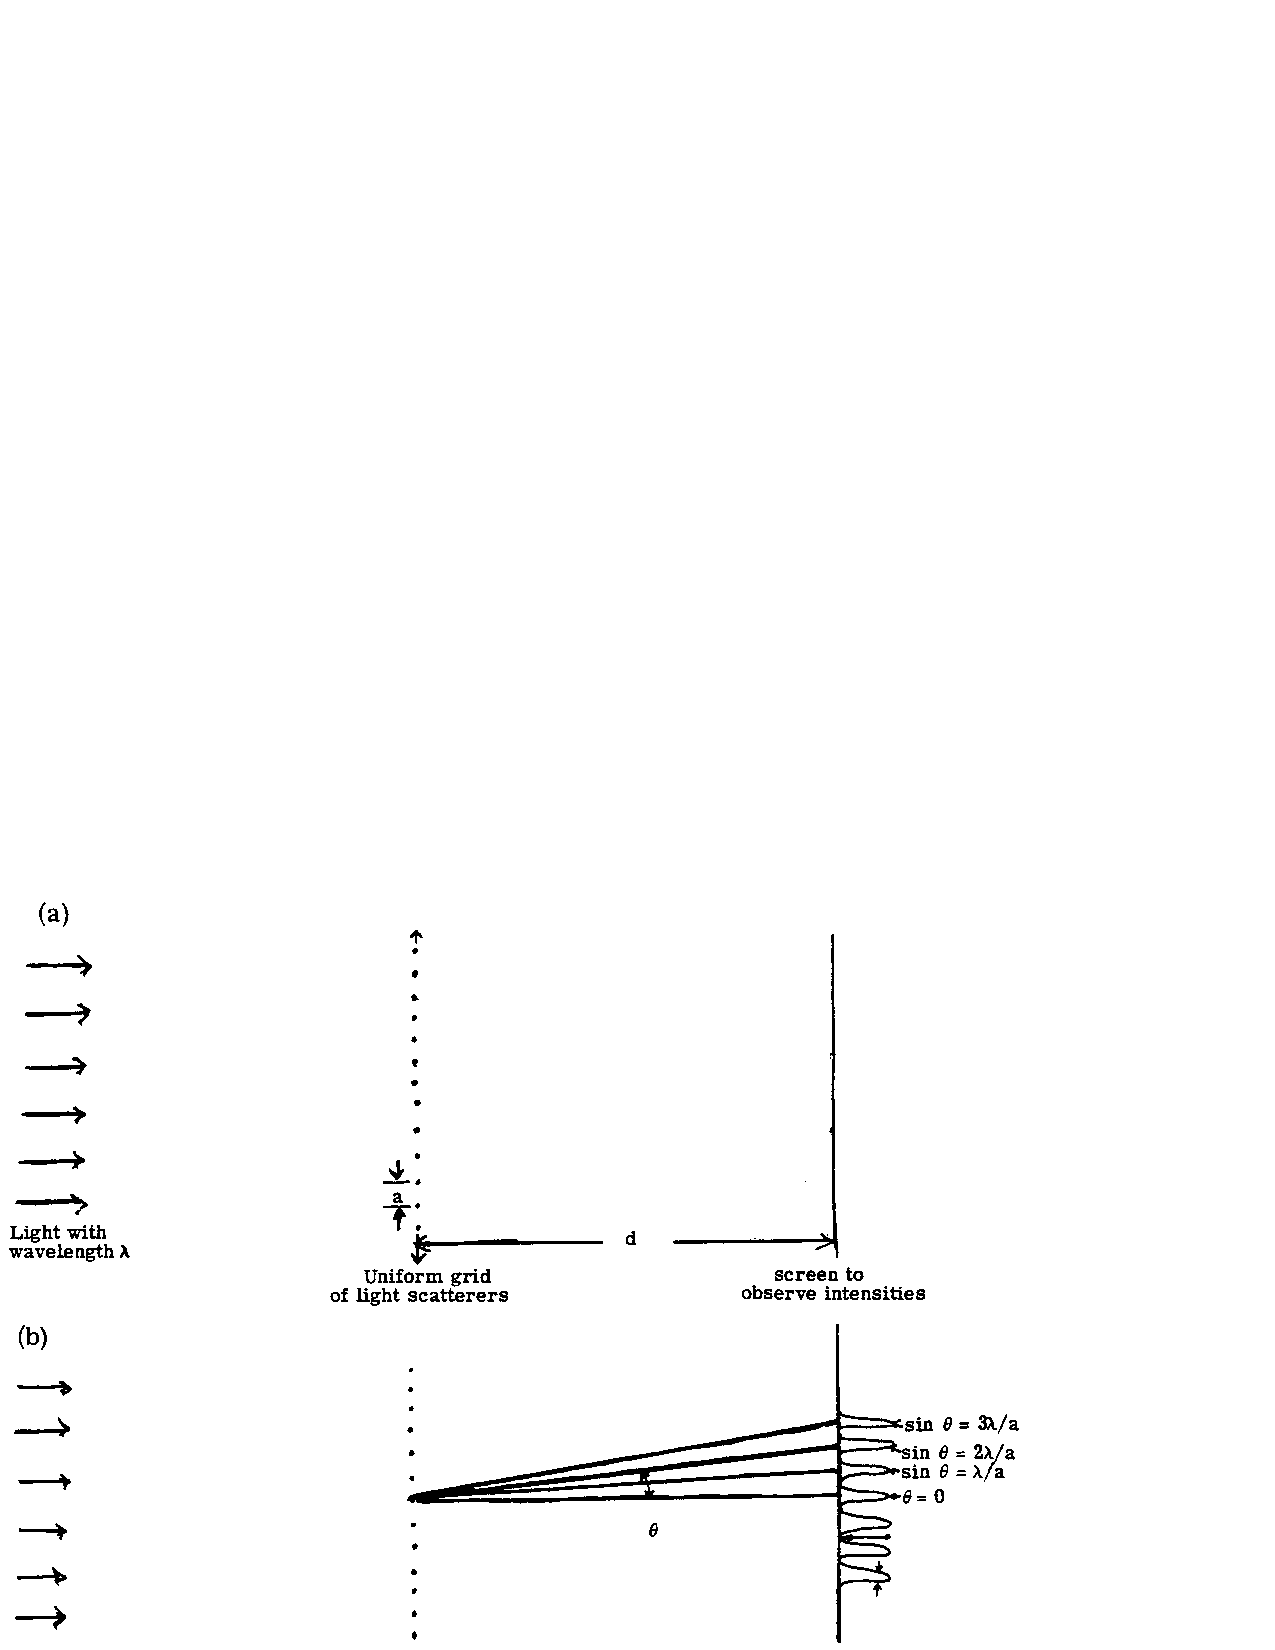
\includegraphics[scale=0.75]{fig1-01}
\caption{Diffraction of light through a grating.}
\label{fig1-1}
\end{figure}
\noindent
With a set of uniformly spaced scatterers, the observed intensities
are sharp spikes at particular angles $\varphi_n$, where $\sin
\varphi_n = n (\lambda/a)$.  To have maxima for $\varphi_n \not= 0$,
we must have $n \lambda / a$, the wavelength must be smaller than the
spacing of the scattering. From measurements of $\sin \varphi_{obs}$
one can calculate $\lambda/a$.  Therefore, knowing the $\lambda$ of
light, we can determine the spacing $a$, or vice verse, knowledge of
the spacing $a$ can be used with $\sin \varphi_{obs}$ to determine
$\lambda$.  A comparison of the observed intensity with that expected
if light did not interfere, is given in Figure \ref{fig1-2}.
\begin{figure}
\begin{center}
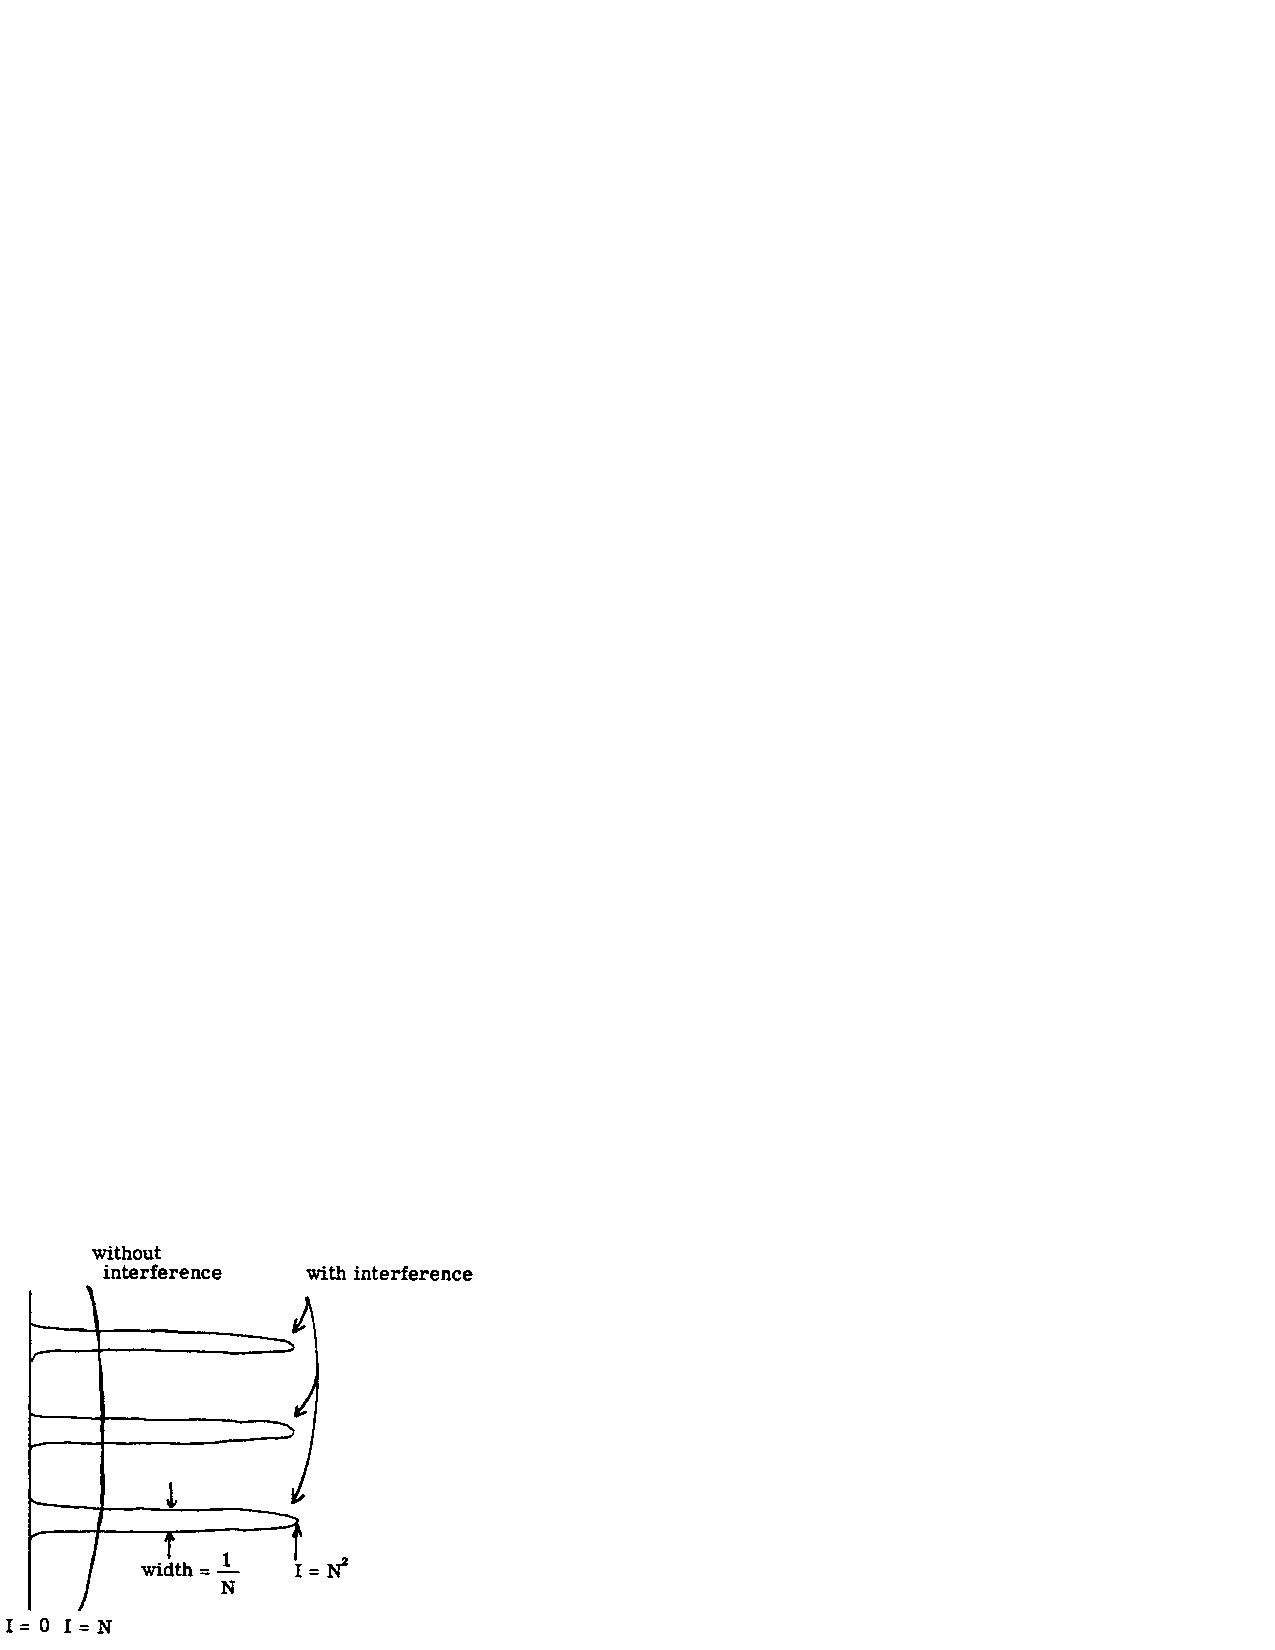
\includegraphics{fig1-02}
\end{center}
\caption{Observed intensities if light did not interfere.}
\label{fig1-2}
\end{figure}

A particularly exciting application to these ideas occurred around
1912.  By that time, a number of scientists believed that x-rays were
electromagnetic waves like light but with very short wavelengths,
$\lambda \approx 1$\AA.  If so, they should exhibit diffraction, if a
grating could be found having equally spaced scatterers with uniform
separation of $\approx 1$\AA. In addition, by 1912 a number of scientists
were convinced that atoms do exist, rather than being just theoretical
constructs, and that crystals might consist of uniformly spaced atoms
having separations of a few angstroms. Von Laue, an expert on
diffraction theory, suggested the experiment of exposing of crystal to
a beam of x-rays and looking for diffraction spikes. After a couple of
years of work, the experiments were successful, proving both the wave
nature of x-rays and the existence of ordered atoms in crystals. Since
then, such x-ray diffraction studies have led to enormous advances in
our atomic-level understanding of matter.

\subsection{Electrons}

The critical experiment establishing the wave nature of electrons is
that a crystal diffracts a beam of electrons in exactly the same way
as it diffracts a beam of X-rays, as illustrated in Figure
\ref{fig1-3}. Thus, electrons must be described as waves.
\begin{figure}
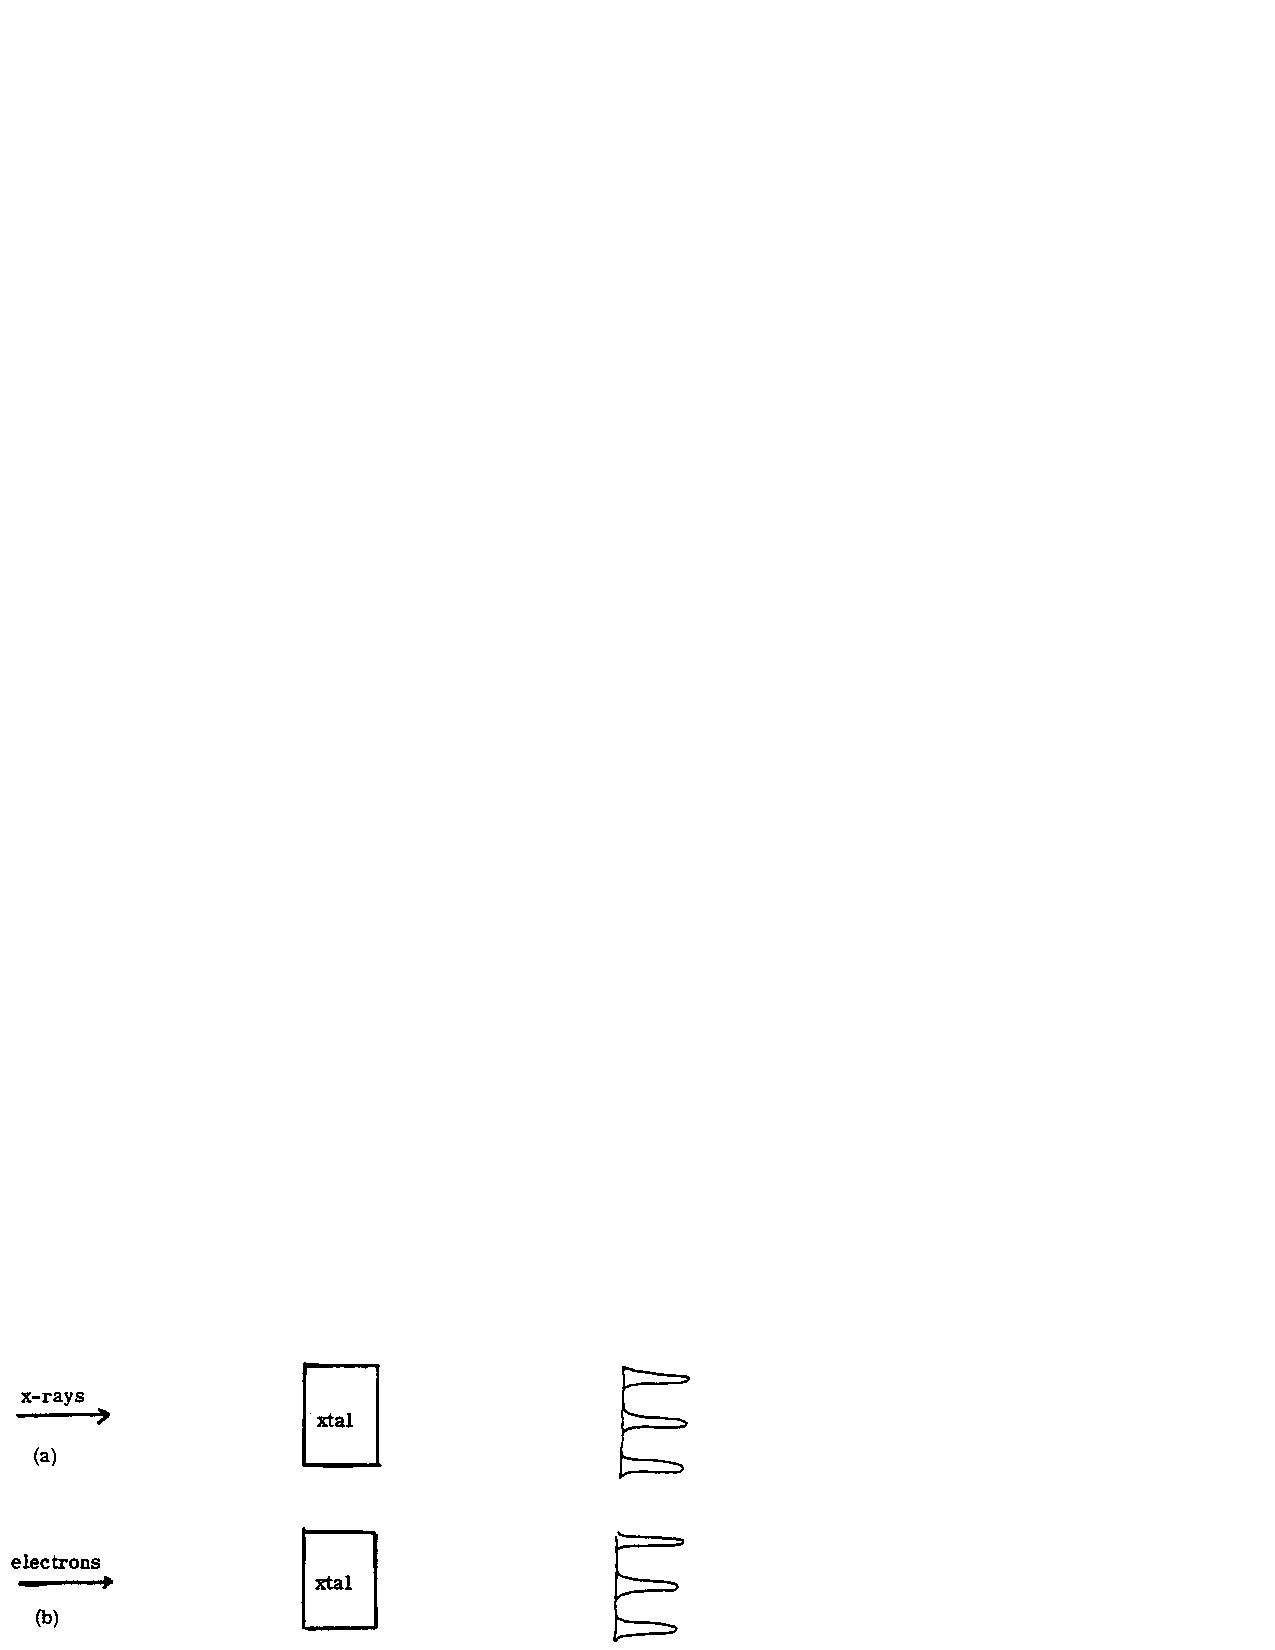
\includegraphics{fig1-03}
\caption{Diffraction of electrons.}
\label{fig1-3}
\end{figure}


This experiment was carried out in 1928 as a test of the ideas arising
from the theorists developing quantum mechanics. Earlier experiments
had, in fact, observed what is now recognized as diffraction; however,
the experiments were not properly interpreted.  Indeed, from these
observations, one can determine the relation between the wave
properties and particle properties of electrons, namely,
\begin{equation}
p = {h \over \lambda} ,
\end{equation}
where $p = \sqrt{2mE}$ is the momentum of the electron and $E$ is the
kinetic energy of the electron, $h$ is a constant, Planck's, and
$\lambda$ is the wavelength of the electrons, obtained from the
spacing of the diffraction peaks.

Based on this and other experiments, we now know that electrons should
be described as wavefunctions, $\psi(x,t)$, where the probability,
$P$, of observing the electrons at some point $x$ is proportional to
the square of the wavefunction,
\begin{equation}
P(x) = \langle \left[ \psi (x,t) \right]^2 \rangle_t .
\end{equation}
The consequences of this will be pondered in the next section.

\subsection{The Schr\"odinger Equation}

In the 1920's, a number of experiments, such as electron diffraction,
showed that matter exhibits interference phenomena just as does
light. This led to the idea that matter, like light, should be
described by an amplitude function, $\psi ( {\bf r} , t)$, called a
wavefunction, such that superposition of two systems $\psi_1$ and
$\psi_2$ leads to superposition of the amplitudes
\begin{equation}
\psi = \psi_1 + \psi_2 
\label{eqno1-3}
\end{equation}
but such that the probability of finding the total system with
particular coordinates {\bf r} and $t$ is given by the, absolute,
square of this amplitude.
\begin{equation}
P( {\bf r} , t) = \vert \psi ( {\bf r} , t ) \vert^2 = \psi ^* ( {\bf r} , 
t ) \psi ( {\bf r} , t ) .
\label{eqno1-4}
\end{equation}
Combining equations (\ref{eqno1-3}) and (\ref{eqno1-4}), leads to
\begin{equation}
P (r , t) = \psi^*_1 \psi_1 + \psi^*_2 \psi_2 + \psi^*_1 \psi_2 + \psi^*_2 
\psi_1 ,
\end{equation}
and hence, interference effects, as observed.

Putting these ideas together, leads to the basic postulate of quantum
mechanics. That is, every physical system is described in terms of a
wavefunction $\psi$ containing all observable information about the
system. This wavefunction is probability amplitude, meaning that a
superposition of states of the system leads to a superposition of the
amplitudes,
\begin{equation}
\psi = \sum_{i} \psi_i .
\label{eqno1-5}
\end{equation}
As part of this basic postulate, we assume that if $\psi_1$ and
$\psi_2$ are two acceptable wavefunctions of a system, then
\begin{equation}
\psi = c_1 \psi_1 + c_2 \psi_2 ,
\label{eqno1-6}
\end{equation}
where $c_1$ and $c_2$ are constants, is also an acceptable wavefunction, 
called the \emph{principle of superposition}.

As part of this basic postulate, the probability of the system having
particular coordinates at a particular time is taken as the absolute
square of the wavefunction $| \psi |^2$ as in equation
(\ref{eqno1-4}). Since the total probability of the system being
somewhere is 1, we have the normalization condition of
\begin{equation}
1 = \int P ( {\bf r} , t ) d \tau = \int \psi^* \psi d \tau 
  \equiv \langle \psi | \psi \rangle
\label{eqno1-7}
\end{equation}
where $d\tau$ is the incremental volume element and this integration
goes over all regions of space. The normalization of the wavefunction
is independent of time, being always unity.

The above postulate implies that anything we can know about the system
must be extracted from the wavefunction. Thus, the wavefunction at
some future time, $t_0 + \delta t$, is completely determined by the
form of the wavefunction at time $t_0$. In other words, there must be
some rule or formula relating
\begin{equation}
\psi ( {\bf r} , t_0 + \delta t ) \equiv \varphi_1 ( {\bf r} )
\end{equation}
to
\begin{equation}
\psi ( {\bf r} , t_0 ) \equiv \varphi_0 ( {\bf r} ).
\end{equation}
Such an association of functions is generally called a transformation
and is denoted as
\begin{equation}
\varphi_1 ( {\bf r} ) = {\hat{A}}_{10} \varphi_0 ( {\bf r} ).
\end{equation}
where ${\hat A}_{10}$ is referred to as the operator effecting the
particular transformation from state $\varphi_0$ to state $\varphi_1$.
Similarly, the time derivative of the wavefunction at time $t_0$,
$\partial \psi / \partial t$, must be determined by the form of the
wavefunction at time $t_0$, and hence we can write
\begin{equation}
\left[ {\partial \psi \over \partial t} \right]_{t_0} = {\hat B} \psi ( 
{\bf r} , t_0 ),
\label{eqno1-8}
\end{equation}
where ${\hat B}$ is called the time evolution operator.  For
convenience, we replace ${\hat B}$ with ${\hat H} = i \hbar {\hat B}$,
where $H$ is referred to as the Hamiltonian.  Thus, equation
(\ref{eqno1-8}) becomes
\begin{equation}
i \hbar {\partial \psi \over \partial t} = {\hat H} \psi ,
\label{eqno1-9}
\end{equation}
which is known as the time-dependent Schr\"odinger equation.  In
equation (\ref{eqno1-9}), $i = \sqrt{-1}$, $\hbar$ is Planck's
constant, 1.054589 $10^{-27}$ erg sec, and $H$ has the dimensions of
energy. Actually, the original Planck's constant $\hbar$ is $h = 2 \pi
\hbar$.  However, we will use only $\hbar$ and refer to it as Planck's
constant.

Since equation (\ref{eqno1-9}) must also apply to any superposition of
wavefunctions (\ref{eqno1-6}), $H$ must be a linear operator
\begin{equation}
H (  \psi_1 + \psi_2 ) = H \psi_1 + H \psi_2 .
\label{eqno1-10}
\end{equation}
From equation (\ref{eqno1-9})
\begin{equation}
i \hbar {\partial \over \partial t} \psi = c_1 \left[ i \hbar {\partial 
\psi_1 \over \partial t} \right] + c_2 \left[ i \hbar {\partial \psi_2 
\over \partial t} \right] = c_2 H \psi_1 + c_2 H \psi_2,
\end{equation}
where equation (\ref{eqno1-9}) was applied to $\psi_1$ and $\psi_2$,
respectively.  Applying equation (\ref{eqno1-9}) directly to $\psi$
leads to
\begin{equation}
i \hbar {\partial \over \partial t} \psi = H \left( c_1 \psi_1 + c_2 \psi_2 
\right)
\end{equation}
and hence equation (\ref{eqno1-10}).  We find that the operator ${\hat
H}$ depends upon the nature of the system and that it is, in general,
a function of both position {\bf r} and time $t$.

If the Hamiltonian $\hat H$ is independent of time, then the solutions 
have the form
\begin{equation}
\psi ( {\bf r} , t ) = \varphi ( {\bf r} ) T ( t ).
\label{eqno1-11}
\end{equation}
where
\begin{equation}
{\partial T \over \partial t} = - i \omega T ( t )
\label{eqno1-12}
\end{equation}
and
\begin{equation}
{\hat H} ( {\bf r} ) \varphi ( {\bf r} ) = \hbar \omega \varphi ( {\bf 
r} ).
\label{eqno1-13}
\end{equation}
Equation (\ref{eqno1-12}) has the solution
\begin{equation}
T ( t ) = e^{- i \omega t} ,
\label{eqno1-14}
\end{equation}
so that equation (\ref{eqno1-11}) becomes
\begin{equation}
\psi ( {\bf r} , t ) = \varphi ( {\bf r} ) e^{- i \omega t},
\end{equation}
where $\varphi ( {\bf r} )$ is yet to be determined from equation
(\ref{eqno1-13}).

At this point we recall the quantum mechanical interpretation of two 
experiments. In the photoelectric experiment, light behaves as a stream 
of particles, called photons, each having a quantum of energy
\begin{equation}
E = \hbar \omega , 
\label{eqno1-15}
\end{equation}
where
\begin{equation}
\omega = 2 \pi \nu = {2 \pi c \over \lambda}
\end{equation}
is the angular frequency of the light. This suggests that the $\hbar
\omega$ in equation (\ref{eqno1-13}) be considered as the energy in
equation (\ref{eqno1-15}). In electron diffraction, the diffraction
pattern for electrons with momentum $p$ and energy $E$ is equivalent
to the diffraction pattern for light with wave vector
\begin{equation}
k = {2 \pi \over \lambda}
\end{equation}
and angular frequency $\omega$, where $\omega$ is given by equation
(\ref{eqno1-14}) and $k$ is given by $p = \hbar k$.  Thus, we postulate
that the energy and frequency are always related by equation
(\ref{eqno1-15}), leading to
\begin{equation}
\psi ( {\bf r} , t ) = \varphi ( {\bf r} ) e^{-{i E t \over \hbar}}
\end{equation}
\begin{equation}
{\hat H} ( {\bf r} ) \varphi ( {\bf r} ) = E \varphi ( {\bf r} ).
\label{eqno1-16}
\end{equation}
The latter equation, (\ref{eqno1-16}), is known as the
time-independent Schr\"odinger equation, and is the fundamental
equation determining chemical bonding.

\subsection{The Form of the Hamiltonian}

In equation (\ref{eqno1-16}) we see that there is a relationship
between the operator ${\hat H}$ and the total energy of the system,
$E$. In classical mechanics, the operator associated with the total
energy of the system is the Hamiltonian $H^{cl}$, which is given by
\begin{equation}
H^{cl} = T^{cl} + V^{cl}
\label{h_cl}
\end{equation}
for nondissipative systems, where $T^{cl}$ and $V^c$ are the kinetic
and potential energies. We will postulate that there are quantum
mechanical operators ${\hat T}$ and ${\hat V}$, corresponding to the
classical quantities $T$ and $V$, such that the quantum mechanical
operator ${\hat H}$ is given by ${\hat H} = {\hat T} + {\hat V}$, and
we will refer to ${\hat H}$ as the Hamiltonian operator.  For a system
in which the classical potential $V^{cl}$ is velocity-independent,
that is, a function of the coordinates of the paxticle only, we will
postulate that the quantum mechanical operator corresponding to $V (
{\bf r} )$ is just the classical function
\begin{equation}
{\hat V} ( {\bf r} ) = V ( {\bf r} )^{cl}.
\label{eqno1-17}
\end{equation}
Thus, for the hydrogen atom,
\begin{equation}
{\hat V} (r) = - {e^2 \over r} .
\end{equation}
For a particle moving in a potential $V^{cl}({\bf r})$, the kinetic
energy, classically, is
\begin{equation}
T^{cl} = {1 \over 2m} p^2 .
\label{eqno1-18}
\end{equation}
where $p = mv$ is the momentum of the particle.  We will postulate
that the quantum mechanical Hamiltonian operator corresponding to
equation (\ref{eqno1-17}) is
\begin{equation}
{\hat T} = {1 \over 2m} {\hat p}^2 ,
\end{equation}
where ${\hat p}$ is the quantum mechanical operator corresponding to the 
momentum.

Now we need the form of the quantum mechanical momentum operator,
${\bf{\hat p}}$. A plane wave of wave vector $k$ and frequency 
$\omega$ has the form
\begin{equation}
\varphi(x ,t) = e^{i(kx - \omega t)},
\end{equation}
and hence the wave vector is given by
\begin{equation}
k = {1 \over \varphi} \left[ {1 \over i} {d \varphi \over dx} 
\right].
\end{equation}
From the diffraction experiments, it was found that $p = \hbar k$, leading to
\begin{equation}
p = {1 \over \varphi} \left[ {\hbar \over i} {d \varphi \over dx} \right].
\end{equation}
Thus, we postulate that the momentum operator ${\hat p}_x$ corresponding to 
momentum in the $x$ direction is given by
\begin{equation}
{\hat p}_x = {\hbar \over i} {\partial \over \partial x}
\label{eqno1-19a}
\end{equation}
and similarly, for the other directions
\begin{equation}
{\hat p}_y = {\hbar \over i} {\partial \over \partial y}
\label{eqno1-19b}
\end{equation}
and
\begin{equation}
{\hat p}_z = {\hbar \over i} {\partial \over \partial z}.
\label{eqno1-19c}
\end{equation}
Just as the classical momentum is a vector quantity, the three
quantities in equations (\ref{eqno1-19a})--(\ref{eqno1-19c}) are
considered as the three components of a vector operator
\begin{equation}
{\hat p} = {\hbar \over i} \nabla
\end{equation}
where $\nabla$ is the gradient operator.

Now we construct the kinetic energy operator. Since
\begin{equation}
\nabla^2 = \nabla \cdot \nabla = \left[ {\partial^2 \over \partial x^2} + 
{\partial^2 \over \partial y^2} + {\partial^2 \over \partial z^2} \right],
\end{equation}
we obtain
\begin{equation}
{\hat p}^2 = {\hat{\bf p}} \cdot {\hat{\bf p}} = \left[ {\hbar \over i} 
\nabla \right] \cdot \left[ {\hbar \over i} \nabla \right] = - \hbar^2 
\nabla^2 = - \hbar^2 \left[ {\partial^2 \over \partial x^2} + {\partial^2 
\over \partial y^2} + {\partial^2 \over \partial z^2} \right] ,
\end{equation}
and hence,
\begin{equation}
{\hat T} = {1 \over 2m} {\hat p}^2 = - {\hbar^2 \over 2m} \nabla^2.
\label{eqno1-20}
\end{equation}
From equation (\ref{h_cl}), (\ref{eqno1-17}), and
(\ref{eqno1-20}), we obtain
\begin{equation}
{\hat H} = - {\hbar^2 \over 2m} \nabla^2 + V ( {\bf r} )
\label{eqno1-21}
\end{equation}
as the explicit form of the Hamiltonian for a particle of mass $m$ 
moving in a potential $V ( {\bf r} )$.

Basically, the Schr\"odinger equation (\ref{eqno1-9}) arises from
considering the time evolution of a system, and the Hamiltonian ${\hat
H}$ describes how the system changes with time. If we change the
system, say, by applying an electric or magnetic field, this change is
manifested by a change in the Hamiltonian ${\hat H}$. Such changes in
${\hat H}$ lead to change in $\psi$.  With suitably ingenious
experiments, it is often possible to determine something about how
$\psi$ changes in response to the field and, thereby something about
the form of $\psi$ before changing ${\hat H}$. In this way, we can
determine various properties of $\psi$.  Ultimately, each physical
property can be related somehow to some type of change in the
Hamiltonian of the system, and hence, to some, Hermitian, operator,
${\hat O}_p = \triangle {\hat H}$.

\subsection{More on the Schr\"odinger Equation}

\subsubsection{The Hilbert Space}

Given any two functions $\psi_1$ and $\psi_2$, we can generate from
equation (\ref{eqno1-5}) as infinite number of wavefunctions $\psi =
C_1 \psi_1 + C_2 \psi_2$ by using various $C_1$ and $C_2$.  In
addition, there is an infinite number of choices for the functions
$\psi_1$ and $\psi_2$.  Even so, the postulates of quantum mechanics
lead to constraints on the functions, and hence, we need not consider
every wavefunction.  For example, from equation (\ref{eqno1-7}) we
need consider only wavefunctions for which the integral of the square
of the wavefunction is unity $\langle \psi | \psi \rangle = 1$. Of
course, given some wavefunction ${\bar{\psi}}$ with
\begin{equation}
\langle {\bar \psi} \vert {\bar \psi} \rangle
   = \int d \tau \vert {\bar \psi} \vert^2 = a
\end{equation}
with finite, nonzero, $a$, we can always define a new function
\begin{equation}
\psi = {{\bar \psi} \over \sqrt{a}}
\end{equation}
that is normalized, i.e., $\langle \psi | \psi \rangle = 1$.  Note
that $a$ can never be negative. On the other hand, we need not
consider any wavefunctions $\psi$ for which the integral $\int d \tau
| \psi |^2$ does not converge. That is, we need deal only with
square-integrable functions. The set of all possible such functions,
satisfying whatever boundary conditions are being imposed, is referred
to as the Hilbert space, for systems having this particular set of
boundary conditions. Thus, the Hilbert space is merely the collection
of all possible wavefunctions for our system.

\subsubsection{Hermitian Operators}

In Section \ref{app-a}, we consider the implications of requiring that
the norm of the wavefunction by unity, $\langle \psi | \psi \rangle =
1$, and hence, independent of time for any superposition of
wavefunctions, $\psi = \psi_i + \psi_j$. The conclusion is that for
all possible functions $\varphi_1$ and $\varphi_2$, the Hamiltonian
operator $H$ must satisfy the condition
\begin{equation}
\int d \tau \left( {\hat H} \psi_i \right) ^* \psi_j = \int d \tau 
\phi_i ^* \left( {\hat H} \psi_j \right),
\end{equation}
which we denote as
\begin{equation}
\langle \left( {\hat H} \psi_i \right) \vert \psi_j \rangle = \langle \psi_i \vert {\hat H} 
\vert \psi_j \rangle .
\end{equation}
Such an operator is called Hermitian.

The expectation value
\begin{equation}
{\langle \psi | {\hat H} | \psi \rangle \over \langle \psi | \psi \rangle}
\end{equation}
of a Hermitian operator is always real, see Section
\ref{app-a}. Hence, the energy
\begin{equation}
E = {\langle \psi | {\hat H} | \psi \rangle \over \langle \psi | \psi \rangle}
\end{equation}
in the Schr\"odinger equation must be real.
In Section \ref{app-a}, we show that the momentum operator
\begin{equation}
{\bf P} = \left( {\hbar \over i} \right) \nabla ,
\end{equation}
and the kinetic energy operator,
\begin{equation}
{\hat T} = \left( {1 \over 2m} \right) {\hat p}^2 ,
\end{equation}
are Hermitian.  Similarly, any function of coordinates, $V(r)$, is
Hermitian, so that the Hamiltonian in equation (\ref{eqno1-21}) is
also Hermitian.

\subsection{Analysis of Kinetic Energy and Potential Energy}

In the previous sections, we have established the Schr\"odinger equation
\begin{equation}
{\hat H} \psi = E \psi,
\label{eqno1-22}
\end{equation}
where 
\begin{equation}
{\hat H} = {\hat T} + {\hat V} ,
\end{equation}
\begin{equation}
{\hat T} = - {\hbar^2 \over 2m} \nabla^2 ,
\end{equation}
and
\begin{equation}
{\hat V} = V ( r ).
\end{equation}
Multiplying both sides of equation (\ref{eqno1-22}) by $\psi ^*$ and
integrating, leads to
\begin{equation}
\langle \psi \vert {\hat H} \vert \psi \rangle = E \langle \psi | \psi \rangle = E ,
\end{equation}
where
\begin{equation}
\langle \psi \vert {\hat H} \vert \psi \rangle = \int d \tau \psi ^* {\hat H} 
\psi
\end{equation}
and $\langle \psi | \psi \rangle = 1$.   Defining the number ${\bar T}$ and 
${\bar V}$ as
\begin{equation}
{\bar T} = \langle \psi \vert {\hat T} \vert \psi \rangle = \int d \tau 
\psi ^* (r) \left[ - {\hbar^2 \over 2m} \nabla^2 \right] \psi 
(r)
\label{eqno1-23}
\end{equation}
and
\begin{equation}
{\bar V} = \langle \psi \vert {\hat V} \vert \psi \rangle = \int d \tau 
\psi ^* (r) V(r) \psi (r),
\label{eqno1-24}
\end{equation}
we see that the total quantum mechanical energy $E$ can be written 
as a sum of quantities $E = {\bar T} + {\bar V}$ interpreted as a 
kinetic energy (${\bar T}$) and potential energy (${\bar V}$)

The quantity (\ref{eqno1-24}) can be rewritten as
\begin{equation}
V = \int d \tau ( r ) \rho(r) V ( r ),
\end{equation}
where
\begin{equation}
\rho ( r ) = \psi ^* ( r ) \psi ( r )
\end{equation}
is the probability of finding the system in the volume element $d \tau$ 
near configuration $r$. Thus, ${\bar V}$ corresponds to the average of 
the classical potential energy, weighted by the probability of
the electron being at any particular position.

As written in equation (\ref{eqno1-8}), ${\bar T}$ does not seem to
bear much relation to the classical kinetic energy.  However, in
Section \ref{app-b} we show that
\begin{equation}
\langle \psi \vert - \nabla^2 \vert \psi \rangle = \langle \vert \nabla 
\psi \vert^2 \rangle,
\end{equation}
so that equation(\ref{eqno1-23}) becomes
\begin{equation}
{\bar T} = {\hbar^2 \over 2m} \langle \vert \nabla \psi \vert^2\rangle 
= {1 \over 2m} \langle \vert {\hbar \over i} \nabla \psi \vert^2 \rangle .
\label{eqno1-25}
\end{equation}
Since ${\hat p} = ( \hbar / i ) \nabla$, we see that
\begin{equation}
{\bar T} = {1 \over 2m} \langle \vert {\hat p} \psi \vert^2 \rangle ,
\end{equation}
which can be compared with the classical kinetic energy,
\begin{equation}
T^{cl} = {1 \over 2m} p^2 ,
\end{equation}
suggesting that $\langle | {\hat p} \psi |^2\rangle$ corresponds to the square
of the classical momentum. Throughout this course, we will find
equation (\ref{eqno1-25}) to be a useful way to think about kinetic
energy. This expression says that big gradients or slopes lead to
large kinetic energy, and hence, the best kinetic energy occurs for
the smoothest functions. Thus, comparing the wavefunctions in Figure
\ref{fig1-4}, all normalized, we see immediately that $\psi_c$ has
the highest ${\bar T}$, which $\psi_a$ has the lowest. Of course,
equation (\ref{eqno1-25}) assumes that $\langle \psi | \psi \rangle = 1$.

\begin{figure}
%%% Warning: figure didn't work %%%
\caption{}
\label{fig1-4}
\end{figure}

The essential difference between classical mechanics and quantum mechanics 
is that in classical mechanics the kinetic energy and the potential energy 
are independent, one is determined by momentum, the other by position.  Whereas 
in quantum mechanics, ${\bar T}$ and ${\bar V}$
are simultaneously determined by the wavefunction, with the kinetic 
energy proportional to the average square of the gradient of the amplitude 
function. It is the balance of trying to find
a wavefunction leading to both the lowest ${\bar T}$ and the lowest ${\bar 
V}$ that is responsible for the stability of quantum mechanical atoms.

\section{The Ground State of Hydrogen Atom}

In this section, we consider the ground state of the hydrogen atom, that 
is, an electron with mass $m$, and charge $-e$ interacting with a nucleus
of infinite mass and charge $+Ze$.  Classically, the energy is given by
\begin{equation}
E = {p^2 \over 2m} - {Ze^2 \over r} ,
\end{equation}
where $r$ is the distance of the electron from the nucleus. Thus, the 
ground state, lowest energy, is for $r = 0$ and $p = 0$, leading to $E = 
-\infty$. That is, the classical $H$ atom collapses to a point.

Quantum mechanically, the Hamiltonian is
\begin{equation}
{\hat H} = - {\hbar^2 \over 2m} \nabla^2 - {Ze^2 \over r},
\end{equation}
and the energy is obtained by solving the Schr\"odinger equation,
\begin{equation}
{\hat H} \psi ( {\bf r} ) = E \psi ( {\bf r} ).
\end{equation}
We will find that the quantum mechanical form of the kinetic energy 
keeps the electron from collapsing into the nucleus.

In these sections, we will obtain the wavefunction $\psi (r)$ for 
the ground state of $H$ atoms. The result is that
\begin{equation}
\psi ( r, \theta, \varphi ) = N_0 e^{- \zeta r} ,
\end{equation}
where 
\begin{equation}
N_0 = \sqrt{{\zeta^3 \over \pi}}
\end{equation}
\begin{equation}
\zeta = {Z \over a_0}
\end{equation}
\begin{equation}
E = - {1 \over 2} Z^2 \left[ {e^2 \over a_0} \right]
\end{equation}
\begin{equation}
a_0 = {\hbar^2 \over me^2}
\end{equation}
Later, we define atomic units where $\hbar = 1$, $m = 1$, and $|e| = 1$.  
In these units, the unit of length is
\begin{equation}
1\ \mathrm{bohr} = 1\ a_0 = {\hbar^2 \over me^2} 
  = 0.529177 \mathrm{\AA},
\end{equation}
and the unit of energy is
\begin{equation}
1\ \mathrm{Hartree} = 1\ h_0 = {e^2 \over a_0} = {me^4 \over \hbar^2}
= 27.2116\ \mathrm{eV}  
= 627.510\ \mathrm{kcal/mol}.
\end{equation}
In these units, the Hamiltonian for $H$ atom becomes
\begin{equation}
{\hat H} = - {1 \over 2} \nabla^2 - {Z \over r},
\end{equation}
the energy becomes
\begin{equation}
E = - {1 \over 2} Z^2,
\end{equation}
and the scale parameter becomes $\zeta = Z$.

Before going into the details of the wavefunctions of the hydrogen atom, we will
consider why such an atom can exist.

\subsection{Atoms Exist!}

In the last section, we found that the classical description of the
atom leads to collapse,
\begin{equation}
T = {1 \over 2m} p^2 \rightarrow 0
\end{equation}
as $p \rightarrow 0$, and
\begin{equation}
V = - {e^2 \over r} \rightarrow - \infty
\end{equation}
as $r \rightarrow 0$.  Therefore, the lowest energy state is for the
electron sitting on the nucleus.  Since the charges cancel, this is
like not having an atom. Now we will look at this problem with quantum
mechanics. A major difference in quantum mechanics is that both $\bar
T$ and ${\bar V}$ are determined by the same quantity, the
wavefunction, whereas in classical mechanics, $T$ and $V$ involved
independent quantities $p$ and $r$. Thus,
\begin{equation}
{\bar V} = \langle \psi \vert - {e^2 \over r} \vert \psi \rangle
\end{equation}
\begin{equation}
{\bar T} = {\hbar^2 \over 2m} \langle \left[ \nabla \psi \right]^2
\rangle. 
\end{equation}

\begin{figure}
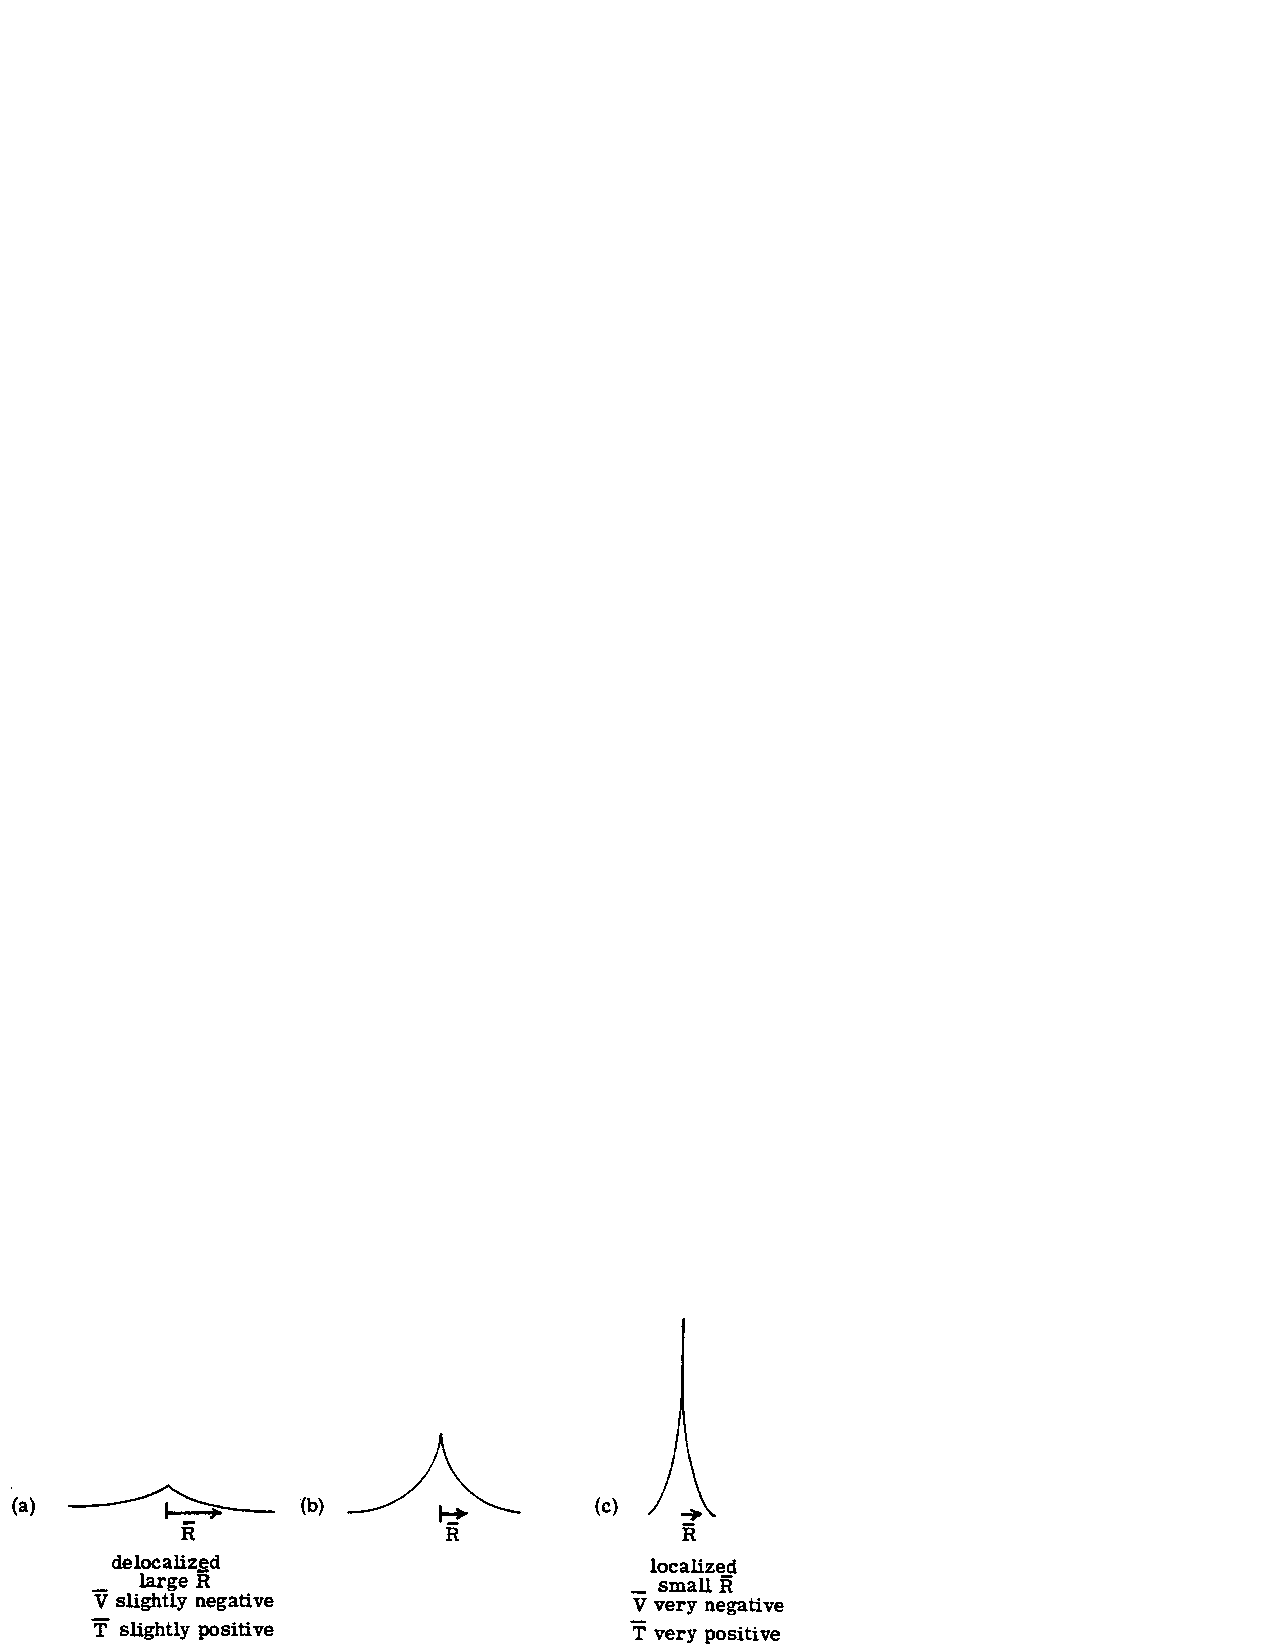
\includegraphics{fig1-05}
\caption{Comparison of wavefunctions with different scales.}
\label{fig1-5}
\end{figure}

Consider now the sequence of similar wavefunctions in Figure
\ref{fig1-5}.  To be specific, consider the normalized function
\begin{equation}
\psi = Ne^{-{r \over {\bar R}}} ,
\end{equation}
where $N = 1 / \sqrt{ \pi {\bar R}^3}$.  Thus, if ${\bar R}$ is very
large, $\psi$ decreases very slowly with $r$, leading to the
delocalized function $a$ in Figure \ref{fig1-5}(a), while with very
small ${\bar R}$, $\psi$ decreases rapidly to zero for small $r$,
leading to the localized function in Figure \ref{fig1-5}(c).
\begin{eqnarray}
\langle \psi^2 \rangle &=& \int^{\pi}_{0} \sin \theta d\theta 
     \int^{\pi}_{- \pi} d\varphi 
     \int^{\infty}_{0} \psi^2 r^2 dr = 4 \pi N^2 \int^{\infty}_{0} r^2 dre^{-2 
\left( {r \over {\bar R}} \right)}\cr 
&=& 4 \pi N^2 \left[ {{\bar R} \over 2} \right]^3 \int^{\infty}_{0} \rho^2 
d \rho e^{- \rho} = \pi N^2 {\bar R}^3 = 1.
\end{eqnarray}
where we used
\begin{equation}
\int^{\infty}_{0} \rho^me^{- \rho} d \rho = m!.
\end{equation}

Clearly, ${\bar V}$ becomes more and more negative, lower energy, as
the electron is localized closer and closer to the nucleus, just as in
classical mechanics, and in the limit the wavefunction leading to the
best ${\bar V}$ is localized at the nucleus, ${\bar R} = 0$. However,
this localization of the electron near the nucleus now leads to a very
large and positive ${\bar T}$. Since ${\bar V}$ and ${\bar T}$ have
opposite effects as the electron is concentrated near the nucleus, we
need to be a little more quantitative in the analysis.

First, we define an average radius ${\bar R}$ as
\begin{equation}
\langle \Phi \vert {1 \over r} \vert \Phi \rangle = {1 \over \bar{R}},
\end{equation}
leading to
\begin{equation}
{\bar V} = - {e^2 \over \bar{R}}.
\label{eqno1-26}
\end{equation}
Consider now, some wavefunction, say $b$, in Figure \ref{fig1-5} as
the reference wavefunction, with ${\bar R} = 1$ in some units, and let
${\bar V}_1$ and ${\bar T}_1$ be the energies for this wavefunction.
Using this reference point, we will examine how ${\bar V}$ and ${\bar
T}$ change as the wavefunction is squeezed or expanded. The technical
term is scaled.

From equation (\ref{eqno1-26}) we see that
\begin{equation}
{\bar V}_{{\bar R}} = \langle \Phi_{{\bar R}} \vert {1 \over r} \vert 
\Phi_{{\bar R}} \rangle = {1 \over {\bar R}} V_1.
\label{eqno1-27}
\end{equation}
In order to see how kinetic energy changes, note that each term has the form
\begin{equation}
\left\langle \left[ {\partial \Phi \over \partial x} \right]\right\rangle^2 ,
\end{equation}
so that
\begin{equation}
{\bar T}_{\bar R} \propto  \left[ {1 \over {\bar R}} \right]^2.
\label{eqno1-28}
\end{equation}
Basically, the gradient is proportional to $1/ {\bar R}$, and hence,
the gradient squared is proportional to $[1/{\bar R}]^2$. Thus, ${\bar
T}$ becomes small for delocalized smooth functions, large ${\bar R}$,
and ${\bar T}$ becomes large, and positive, for localized functions,
small ${\bar R}$.  From equations (\ref{eqno1-27}) and
(\ref{eqno1-28}), we see that
\begin{equation}
{{\bar T}_{\bar R} \over {\bar V}_{\bar R}} = \left[ {1 \over {\bar R}} 
\right] {{\bar T}_1 \over {\bar V}_1}
\label{eqno1-29}
\end{equation}
note that ${\bar T}$ is always positive, and ${\bar V}$ is always negative.

Consider first, the case as ${\bar R} \rightarrow \infty$, then from
equations (\ref{eqno1-27}) and (\ref{eqno1-28}) ${\bar T} \rightarrow
0$, ${\bar V} \rightarrow 0$, and ${\bar E} = {\bar T} + {\bar V}
\rightarrow 0$, as expected.  For sufficiently large ${\bar R}$, that
is, ${\bar R} \gg | {\bar T}_1 / {\bar V}_1 |$, we see from equation
(\ref{eqno1-29}) that $ | {\bar V} | \gg | {\bar T} |$, and hence, the
total energy $E = {\bar T} + {\bar V}$ must be negative. However, for
very small ${\bar R}$, that is, ${\bar R} \ll | {\bar T}_1 / {\bar
V}_1 |$, we see from equation (\ref{eqno1-29}) that $| {\bar T} | \gg |
{\bar V} |$, and hence, the total energy must be positive. Thus, the
energy of the wavefunctions in Figure \ref{fig1-5} must behave, as in
Figure \ref{fig1-6}, as a function of ${\bar R}$, i.e., as a function
of the size of the wavefunction. That is, the lowest energy,
corresponding to the ground state of the atom, occurs at a finite
size,${\bar R} = {\bar R}_{opt}$.  In quantum mechanics the hydrogen
atom is stable.

\begin{figure}
\begin{center}
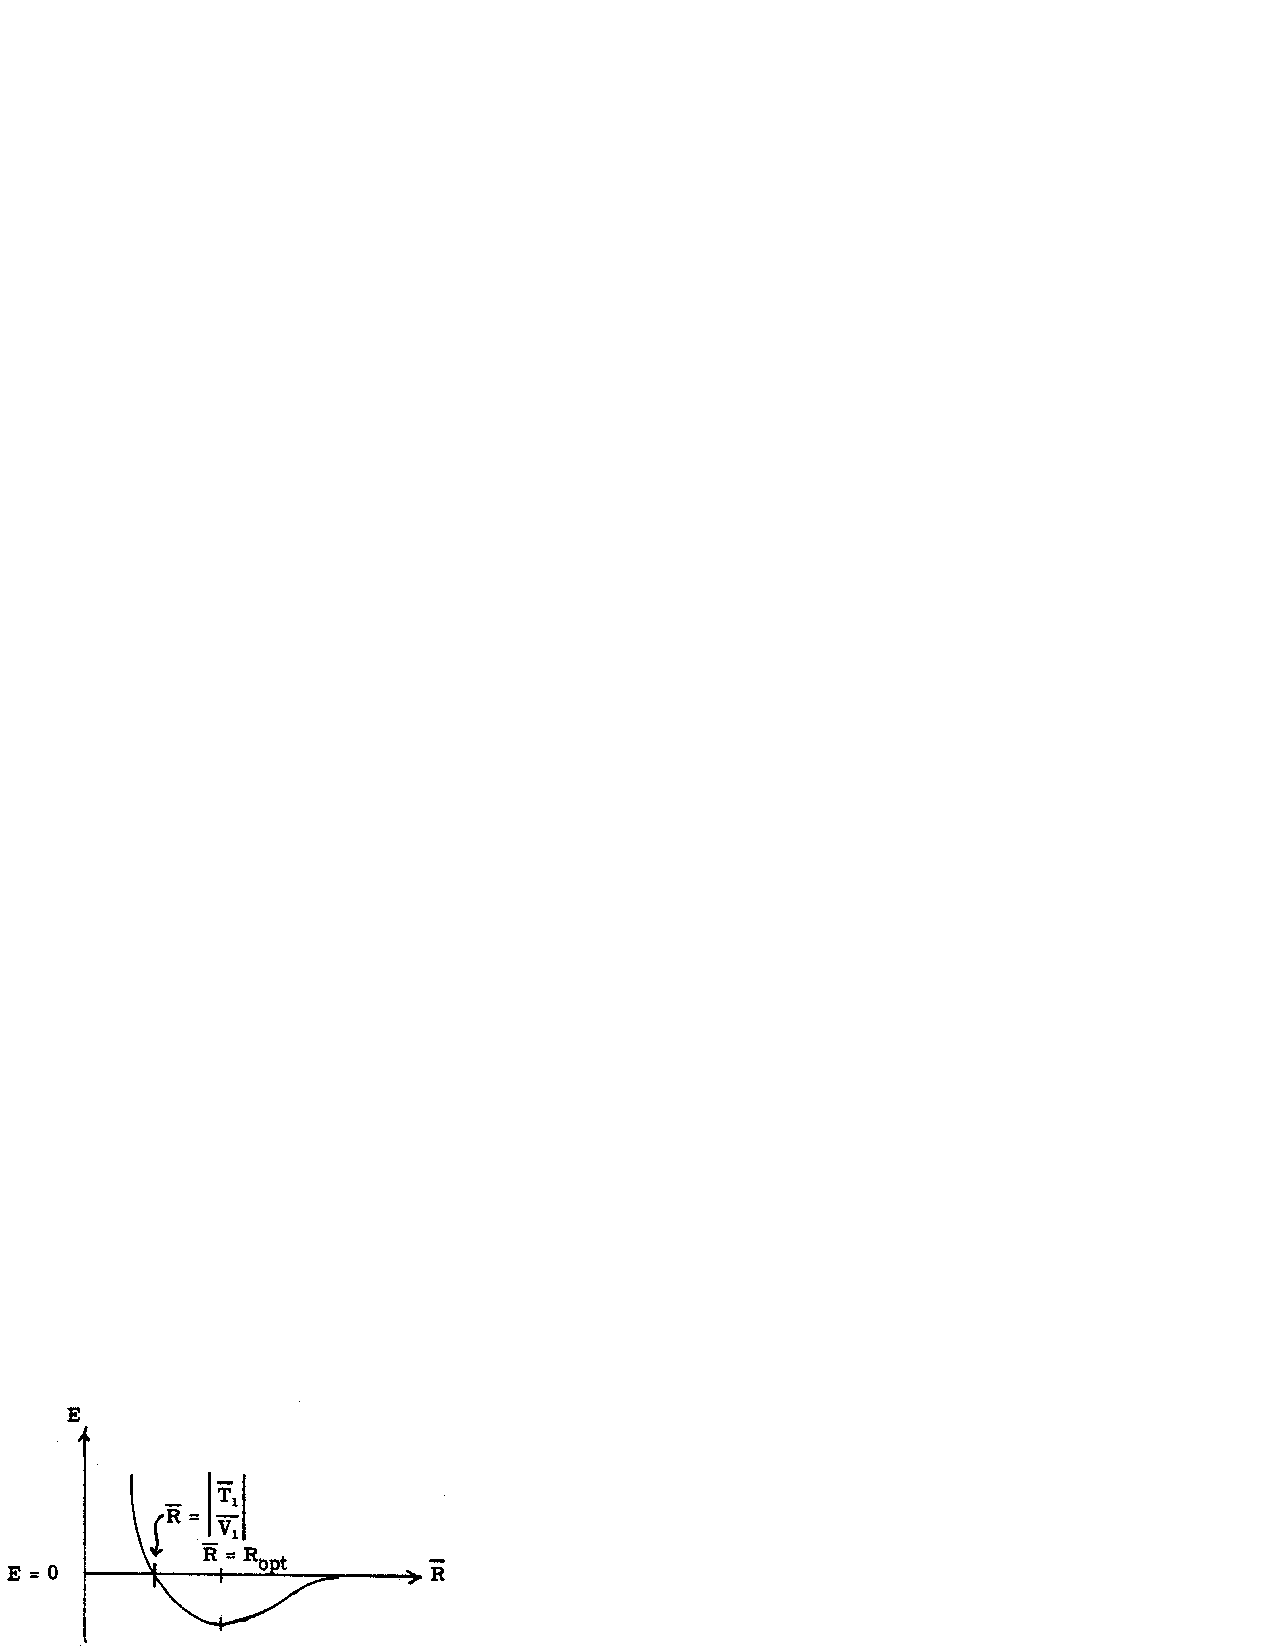
\includegraphics{fig1-06}
\end{center}
\caption{H atom is stable in quantum mechanics.}
\label{fig1-6}
\end{figure}

In the above example, we consider just the stretching and compression
of the one function considered in Figure \ref{fig1-5}. However, the
same result is obtained independent of the shape, namely, the optimum
energy occurs for finite ${\bar R}$, and hence, trying all possible
shapes we will eventually find the optimum wavefunction and its
optimum ${\bar R}$. This optimum wavefunction is discussed in the next
section.

Summarizing the above discussion, we find that the potential energy wants 
the wavefunction to be localized at the nucleus. Thus, starting with a 
delocalized wavefunction, Figure \ref{fig1-5}(a), the total energy drops as the 
wavefunction is localized closer to the nucleus. This localization, that 
aids the potential energy, leads concomitantly to a more repulsive 
kinetic energy.  However, for sufficiently diffused wavefunctions, potential 
energy always wins. We are assuming here, Coulombic attractions. On the other 
hand, the kinetic energy increases quadratically as the wavefunction is 
compressed, while the potential energy only drops linearly, so that 
eventually the increase in kinetic energy will prevent any further 
contraction of the wavefunction. For the optimum wavefunction, there 
is a balance in these potential energy and kinetic energy terms. One 
might say that kinetic energy provides a pressure that keeps the atom 
from collapsing.

\subsection{The Ground State Wavefunction}

Now we wish to obtain the wavefunction $\psi (r)$ of the ground state of $H$
atom,
\begin{equation}
H \psi ( {\bf r} ) = E \psi ( r ),
\label{eqno1-30}
\end{equation}
where
\begin{equation}
H = - {\hbar^2 \over 2m} \nabla^2 - {Ze^2 \over r}.
\label{eqno1-31}
\end{equation}

The Hamiltonian in equation (\ref{eqno1-31}) is independent of
orientation of the atom in space, and hence, the eigenfunctions will
have the form
\begin{equation}
f (r) Z (\theta, \varphi),
\label{eqno1-32}
\end{equation}
where $f$ is a function of $r$ only, and $Z(\theta,\varphi)$ is a function 
of angular coordinates only. Since kinetic energy favors having smooth 
wavefunctions, the ground state wavefunction should be
as devoid of wiggles as possible. Thus, we will take $Z(\theta,\varphi)$ 
as a constant leading to
\begin{equation}
-{\hbar^2 \over 2m} \nabla^2 f ( r ) + {Ze^2 \over r} f ( r ) = E f ( r 
)
\label{eqno1-33}
\end{equation}
for the Schr\"odinger equation.

There are straightforward mathematical techniques for solving equation
(\ref{eqno1-33}).  For example, see Section \ref{app-d}. Here we will
use a physically oriented approach to examine some features of the
solutions.  At $r = \infty$, the potential in equation
(\ref{eqno1-31}) is zero, thus, the bound states of equation
(\ref{eqno1-30}) have negative energy, $E < 0$. Now consider a very
large $r$ so that the Coulomb term is negligible,
\begin{equation}
{Ze^2 \over r} \ll  | E |.
\end{equation}
In this case, the Schr\"odinger equation reduces to
\begin{equation}
- {\hbar^2 \over 2m} \nabla^2 f ( r ) = E f ( r )
\end{equation}
or
\begin{equation}
\nabla^2 f ( r ) = + \zeta^2 f ( r ),
\label{eqno1-34}
\end{equation}
where
\begin{equation}
\zeta^2 = - {2m \over \hbar^2} E
\label{eqno1-35}
\end{equation}
note that $E$ is negative and, hence, $\zeta$ is real. Consider a
point along the positive $x$ axis. Since $r$ is very large,
\begin{equation}
\left( {\partial f \over \partial y} \right) \approx 0
\end{equation}
and
\begin{equation}
\left( {\partial f \over \partial x} \right) \approx 0.
\end{equation}
Thus, equation (\ref{eqno1-34}) becomes
\begin{equation}
+ {\partial^2 f \over \partial x^2} = \zeta^2 f.
\end{equation}
Consequently, $f = e^{-\zeta x}$, where this is also a solution, but this 
function is not normalizable.  Since $f$ is spherically symmetric, the 
wavefunction at very large $r$ is of the form
\begin{equation}
f ( r ) = e^{- \zeta r}.
\label{eqno1-36}
\end{equation}

\begin{figure}
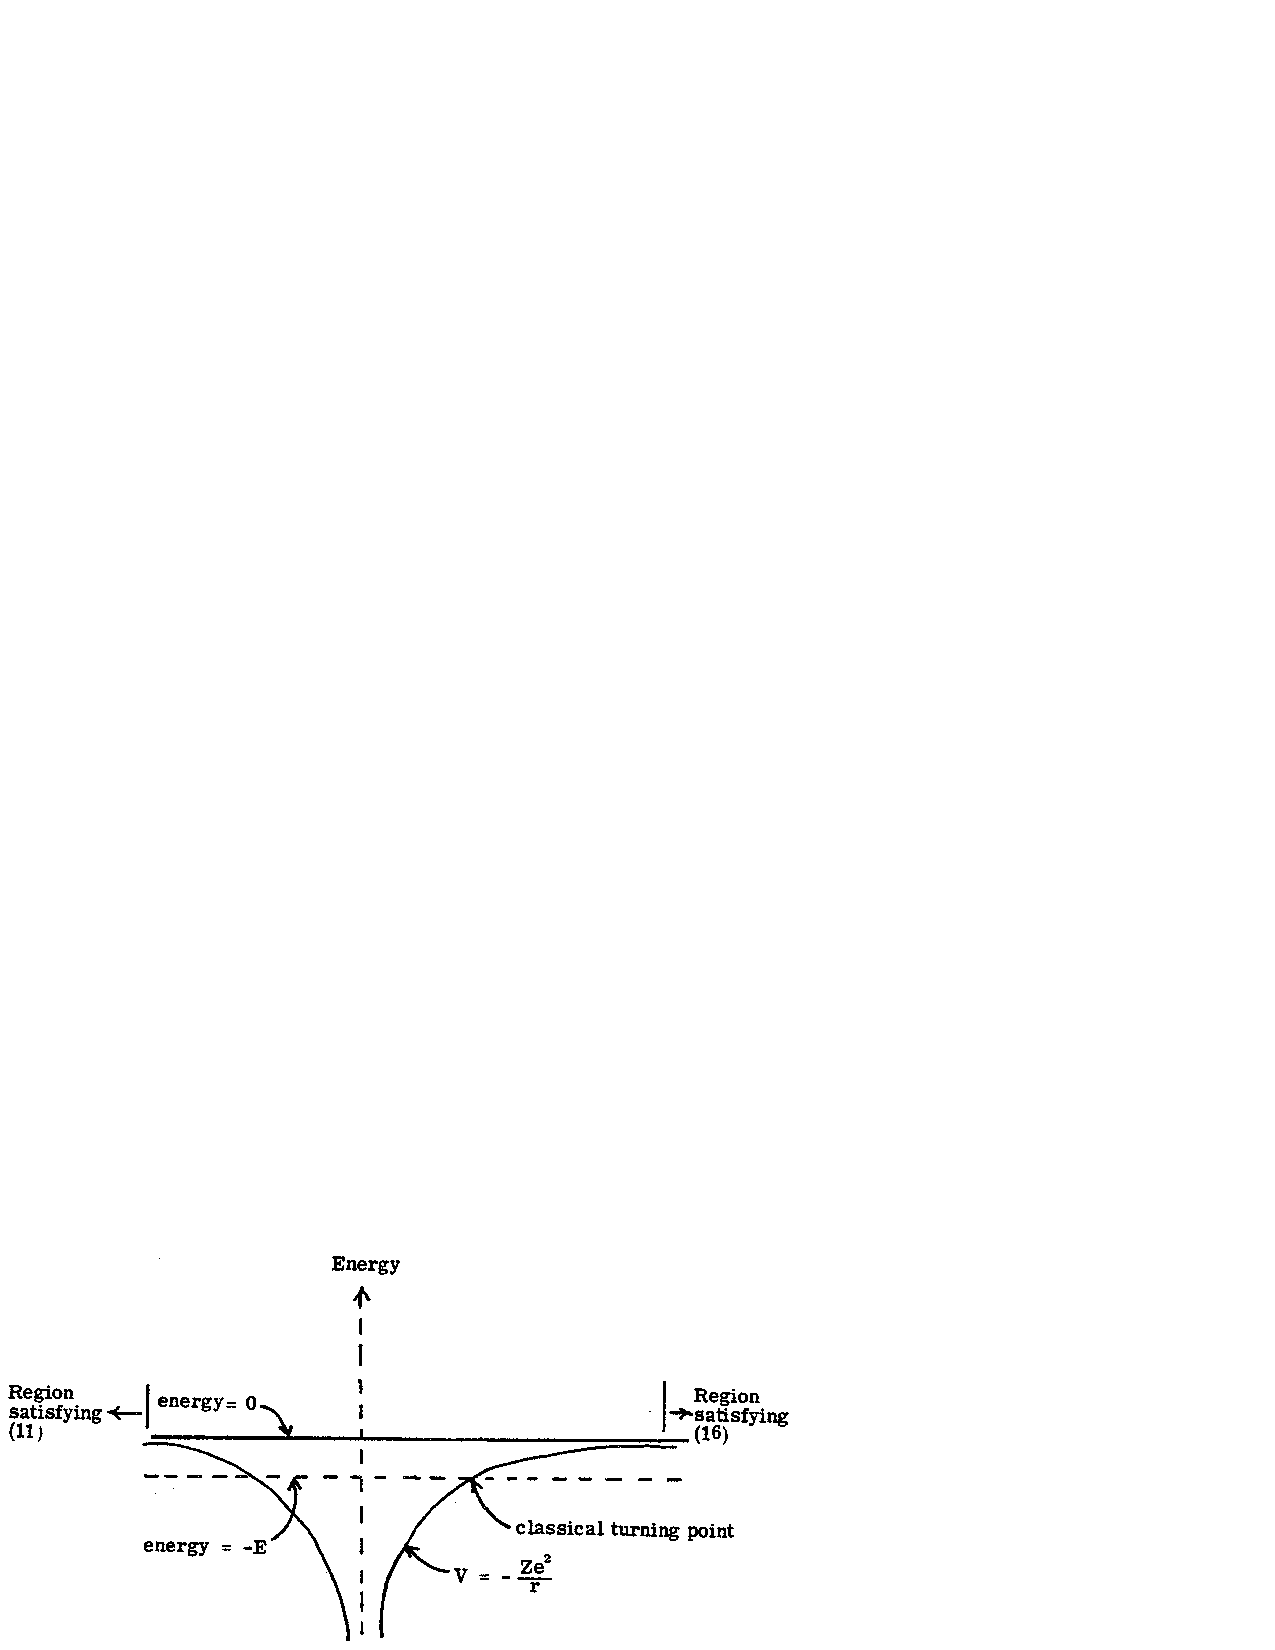
\includegraphics{fig1-07}
\caption{$H$ potential with classical turning points.}
\label{fig1-7}
\end{figure}

In Section \ref{app-d}, we show that the wavefunction (\ref{eqno1-36})
is an eigenfunction of equation (\ref{eqno1-33}) for all $r$ if
$\zeta$ is chosen so that
\begin{equation}
\zeta = {Z \over a_0},
\label{eqno1-37}
\end{equation}
where
\begin{equation}
a_0 = {\hbar^2 \over me^2}.
\label{eqno1-38}
\end{equation}
From equations (\ref{eqno1-35}) and (\ref{eqno1-37}), we have
\begin{equation}
E = - {\hbar^2 \over 2m} \zeta^2 = - {\hbar^2 \over 2m} {Z^2 \over 
a_0^2} = - {1 \over 2} {Z^2e^2 \over a_0},
\end{equation}
and hence,
\begin{equation}
E = - {1 \over 2} Z^2 \left[ {e^2 \over a_0} \right].
\label{eqno1-39a}
\end{equation}
Normalizing the wavefunction (\ref{eqno1-36}) leads to, see Section
\ref{app-d}
\begin{equation}
\psi ( r , \theta, \varphi ) = N_0 e^{-{Zr \over a_0}},
\label{eqno1-39b}
\end{equation}
where
\begin{equation}
N_0 = \sqrt{{Z^3 \over \pi a_0^3}}.
\end{equation}
This wavefunction is plotted in Figure \ref{fig1-8}.

\begin{figure}
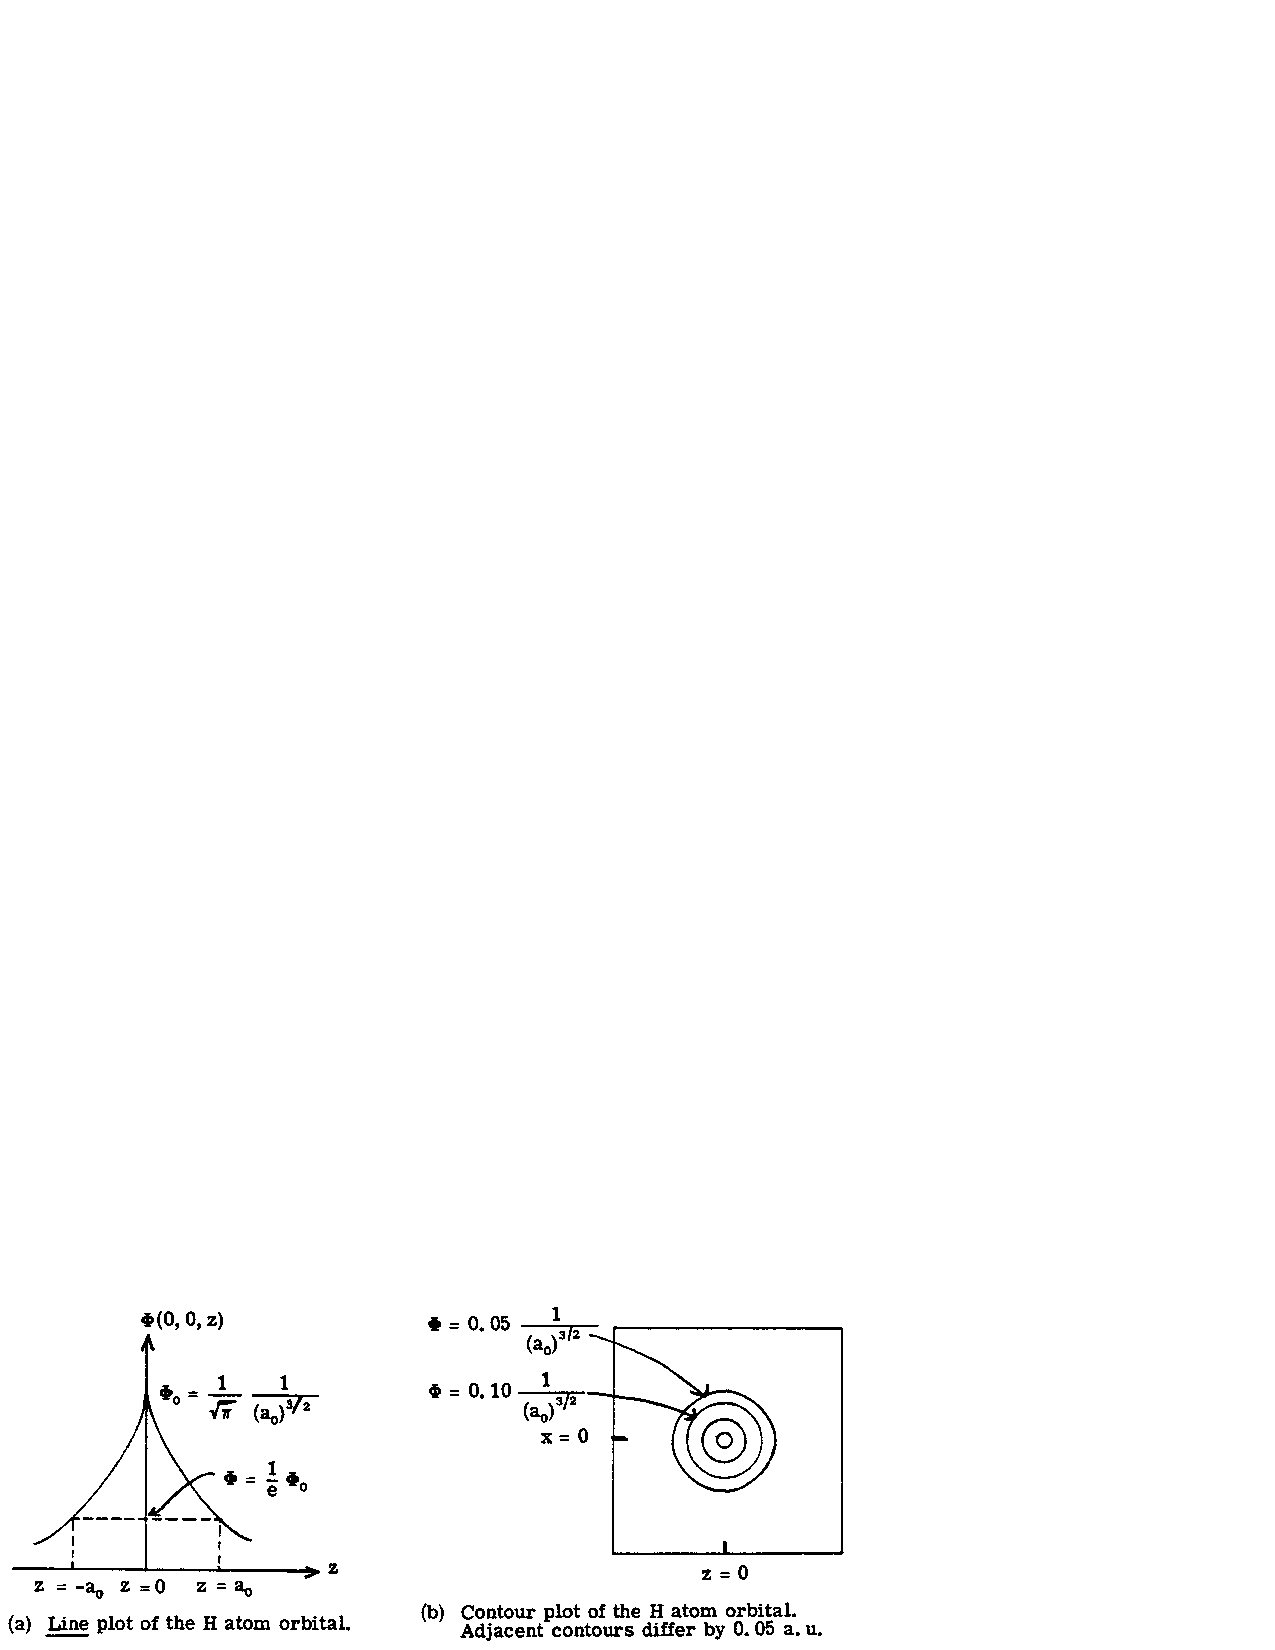
\includegraphics{fig1-08}
\caption{Line (a) and contour (b) plots of the $H$ atom orbital; in
(b), the adjacent contours differ by 0.05 a.u.}
\label{fig1-8}
\end{figure}

The average radius of the wavefunction (\ref{eqno1-38}) is
\begin{equation}
{1 \over \bar{R}} = \langle \psi \vert {1 \over r} \vert \psi \rangle = {Z 
\over a_0},
\end{equation}
so that
\begin{equation}
{\bar R} = {a_0 \over Z},
\end{equation}
where $a_0 = \hbar^2/me^2$ is referred to as the Bohr radius, or more
simply, the Bohr, in honor of Niels Bohr. Substituting into equation
(\ref{eqno1-37}) leads to
\begin{equation}
E = - {1 \over 2} {Ze^2 \over {\bar R}} ,
\label{eqno1-40}
\end{equation}
which can be compared with
\begin{equation}
{\bar V} = \langle \psi \vert - {Ze^2 \over r} \vert \psi \rangle 
= -{Ze^2 \over {\bar R}}.
\end{equation}
Thus,
\begin{equation}
E = {1 \over 2} {\bar V}
\end{equation}
and
\begin{equation}
{\bar T} = E - {\bar V} = - {1 \over 2} {\bar V} = {1 \over 2} {Ze^2 
\over {\bar R}}.
\end{equation}
Equation (\ref{eqno1-40}) provides an easy way to remember the proper
energy expression, it is just half the total potential energy.

For the hydrogen atom, $Z = 1$, the above equations become
\begin{equation}
E = - {1 \over 2} {e^2 \over a_0}
\end{equation}
\begin{equation}
{\bar V} = - {e^2 \over a_0}
\end{equation}
\begin{equation}
{\bar T} = + {1 \over 2} {e^2 \over a_0} = + {\hbar^2 \over 2m} {1 
\over a^2_0},
\end{equation}
where
\begin{equation}
\left\langle {1 \over r} \right\rangle = {1 \over a_0}
\end{equation}
\begin{equation}
\langle \left[ \nabla \varphi \right]^2 \rangle = {1 \over a^2_0}.
\end{equation}

\begin{figure}
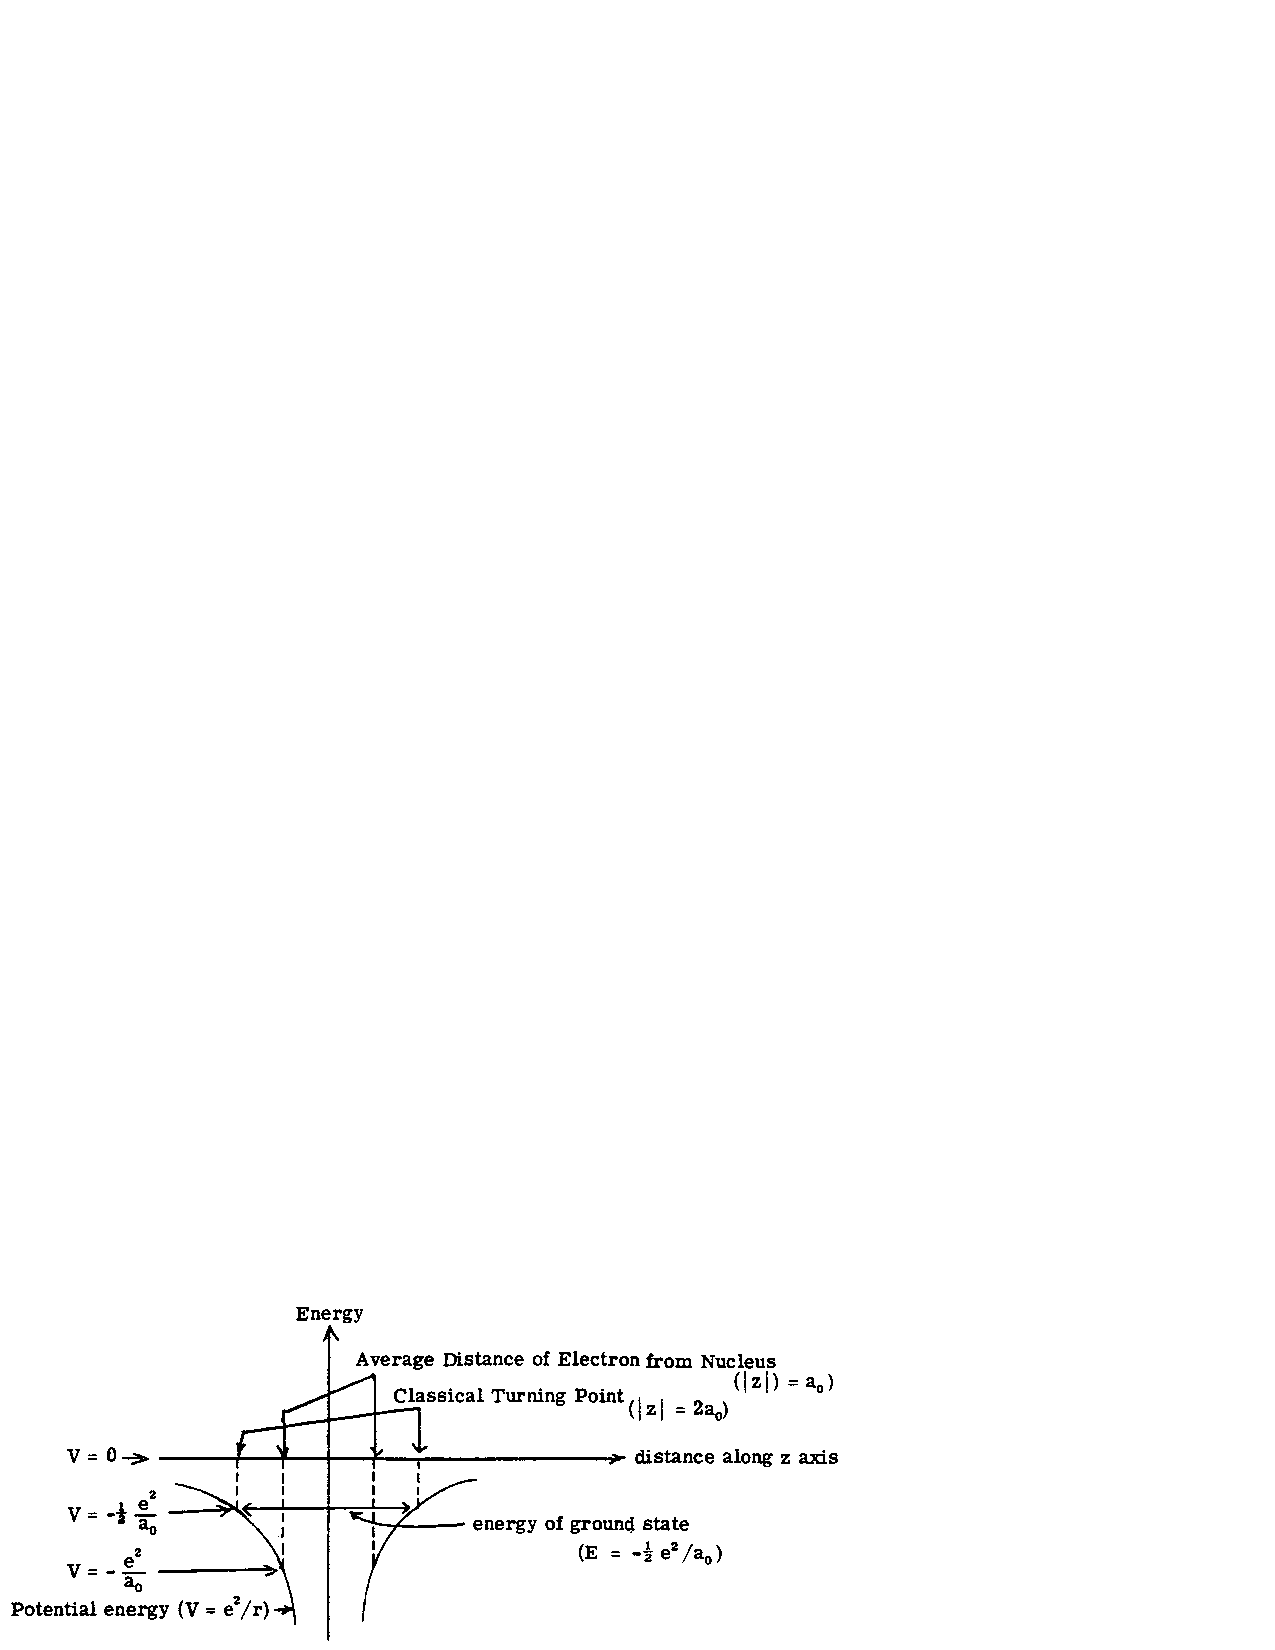
\includegraphics{fig1-09}
\caption{The potential energy as a function of distance.}
\label{fig1-9}
\end{figure}

\noindent
Imagining a classical particle with this same energy $E$ moving in the
potential
\begin{equation}
V(r) = - \left( {e^2 \over r} \right),
\end{equation}
we would find the particle bouncing back and forth from $z = -2a_0$ 
to $z = + 2a_0$.  The kinetic energy is
\begin{equation}
T = E - V = E + {e^2 \over r} = - {e^2 \over 2a_0} + {e^2 \over r}.
\end{equation}
For $r > 2a_0$, we would have $T < 0$, but this is not possible,
classically, since $T = 1/2mv^2$ must be positive. Thus, the classical
limit for the motion of the electron is $|z| = 2a_0$, at which point
the velocity has reduced to zero. In the quantum description, there is
a finite probability, but not large, of the electron being farther
than $2a_0$ from the nucleus.

Note that the wavefunction (\ref{eqno1-39b}) is positive for all
finite $x$, $y$, and $z$.  Since it is never zero for finite
distances, we say that the wavefunction is nodeless.

\subsection{Atomic Units}

As mentioned, the size of the atom is
\begin{equation}
{\bar R} = {a_0 \over Z},
\end{equation}
thus, a natural unit of length for atomic problems is the Bohr radius
\begin{equation}
a_0 = {\hbar^2 \over me^2}.
\end{equation}

The quantity
\begin{equation}
{e^2 \over a_0} = {me^4 \over \hbar^2} 
\end{equation}
in the energy expression, equation (\ref{eqno1-40}) has units of
energy. It is referred to as the Hartree, in honor of D. R. Hartree
who first suggested the atomic system of units,$^3$ and is denoted as
$h_0$,
\begin{equation}
h_0 = {e^2 \over a_0} = {me^4 \over \hbar^2} 
\end{equation}
so that the energy of the hydrogen atom (\ref{eqno1-39b}) becomes
\begin{equation}
E = - {1 \over 2} Z^2 h_0.
\end{equation}
Throughout this course, we will encounter quantities such as $a_0 = 
\hbar/me^2$ corresponding to a length,
\begin{equation}
h_0 = {e^2 \over a_0} = {me^4 \over \hbar^2} 
\end{equation}
corresponding to an energy, and dimensionless quantities such as
\begin{equation}
\alpha = {e^2 \over \hbar c} = { 1 \over 137.03604}
\end{equation}
the fine structure constant.

We will find it convenient to use a particular set of units, called 
atomic units, where $\hbar = 1$, $m_e = 1$, and $|e| = 1$.  Atomic units 
are sometimes called Hartree atomic units to distinguish
them from other occasionally used atomic units, see Section \ref{app-e}.

We use the above unit because they simplify many of the equations of quantum
mechanics and give a reasonable order of magnitude, near unity, for the properties of
molecular systems. Some useful conversion constants are include in
Section \ref{app-f}.

With atomic units, the Hamiltonian for the hydrogen atom becomes
\begin{equation}
H = - {1 \over 2} \nabla^2 - {Z \over r}
\end{equation}
and the ground state wavefunction becomes
\begin{equation}
\psi ( r, \theta, \varphi ) = N_0 e^{-Zr},
\label{eqno1-41}
\end{equation}
where
\begin{equation}
N_0 = \sqrt{{Z^3 \over \pi}}
\end{equation}
and the ground state energy becomes
\begin{equation}
E = - {1 \over 2} Z^2.
\end{equation}

\subsection{Conversion Factors}

In order to compare the results of quantum mechanics, expressed in
atomic units, with those of experiment, expressed in cgs units, it is
necessary to become facile at converting between those units. To do
this simply, it is sufficient to remember a few basic conversions,
e.g., energy and distance, and to rewrite the expressions involving
other quantities in terms of these basic units before
converting. Thus, from equation (\ref{eqno1-41}) the ionization
potential of the ground state of hydrogen atom is
\begin{equation}
\mathrm{IP}_H = {1 \over 2} \left( {e^2 \over a_0} \right).
\end{equation}
In atomic units, this quantity is
\begin{equation}
\mathrm{IP}_H = 0.5\ h_0 ,
\end{equation}
and experimentally, it is known that
\begin{equation}
\mathrm{IP}_H = 13.605805(37)\ \mathrm{eV}.
\end{equation}
This is corrected to correspond to a nucleus of infinite mass. Thus,
\begin{equation}
1 h_0 = {e^2 \over a_0} = 27.21161\ \mathrm{eV}.
\end{equation}

Similarly, using the known values of $\hbar$, $m$, and $e$
\begin{equation}
\hbar = 1.0545887(56) \times 10^{-27}\ \mathrm{gm}\ \mathrm{cm}^2\
\mathrm{sec}^{-1}
\end{equation}
\begin{equation}
m_e = 9.109534(47) \times 10^{-28}\ \mathrm{gm}
\end{equation}
\begin{equation}
e = 4.803242(14) \times 10^{-10}\ \mathrm{gm}^{{1 \over 2}}\ 
\mathrm{cm}^{{3 \over 2}}\ \mathrm{sec}^{-1},
\end{equation}
we find that the atomic unit of length is
\begin{equation}
1a_0 = {\hbar^2 \over me^2} =  0.52917704(44)\ \mathrm{\AA}.
\end{equation}

Another useful relation is the fine structure constant
\begin{equation}
\alpha = {e^2 \over \hbar c} = {1 \over 137.03604(11)},
\end{equation}
a dimensionless constant. In atomic units, $e = 1$ and $\hbar =1$, and 
hence, the speed of light is
\begin{equation}
c = 137.03604\ \mathrm{a.u.}
\end{equation}
in atomic units. From the cgs value of $c$,
\begin{equation}
c = 2.99792458(l) \times 10^{10}\ \mathrm{cm}/\mathrm{sec}
\end{equation}
we find the atomic unit of time, denoted as $\tau_0$,
\begin{equation}
\tau_0 = 2.41888 \times 10^{-17}\ \mathrm{sec}.
\end{equation}
The numbers in parentheses indicate the estimated limits of error in the last
digit quoted, the standard deviation.

The biggest disadvantage in using atomic units is that the various 
quantities such as $\hbar$, $e$, and $m_e$ will be missing from the equations, 
making it difficult to convert to cgs units. The best way to convert is to 
rewrite the quantity of interest in terms of energy, length, and velocity 
quantities and then to use the above conversions. For example, what if we 
want to evaluate the Coulomb interaction between $Na^+$ and $Cl^-$ at 10
\AA? We convert $R$ to Bohr
\begin{equation}
R = {10 \over 0.529177} = 18.897\ a_0.
\end{equation}
Since $|e| = 1$, the energy of interaction in atomic units is
\begin{equation}
E = {1 \over R} = - 0.052918\ h_0.
\end{equation}
We can now convert back to electron volts,
\begin{equation}
E = -0.052917 \times 27.2116 = -1.43998\ \mathrm{eV}.
\end{equation}
In general, then
\begin{equation}
E(\mathrm{eV}) = {-14.3998 \over R(A)}.
\end{equation}
It would be instructive to calculate other quantities in terms of atomic 
units. For example, what is the average momentum of the electron in the 
ground state of $H$? In Bohr's model, how
long does it take the electron to orbit the atom?

\section{The Nodal Theorem}

Even without carrying out detailed calculations of the eigenfunctions for 
a system, it is often possible to make some general conclusions concerning 
the ordering of the states by considering their nodal structures, i.e., 
the loci of points for which $\psi = 0$. Here we will
develop some of the general considerations for such analyses.

First, we consider a one-dimensional, one-particle system with Hamiltonian
\begin{equation}
H = - {1 \over 2M} {d^2 \over dx^2} + V( x ),
\end{equation}
where $M = m/\hbar^2$ and $V(x)$ is some function of $x$ depending only 
upon the spatial coordinates. $V(x)$ is independent of momentum and spin, 
and is not an integral operator. If this potential contains bound states, 
then we can prove the nodal theorem. First, the ground
state wavefunction does not change sign, i.e., has no nodes. Secondly, 
the bound state with $n$ sign changes, $n$ nodes, has a lower energy than 
the state with $n + 1$ sign changes, $n + 1$ nodes.

That is,
\begin{equation}
E_0 < E_n
\end{equation}
\begin{equation}
E_n < E_{n+1}
\label{eqno1-42}
\end{equation}
where $n$ is the number of nodal points, internal to the
boundaries. In the case of a sufficiently singular potential, some
inequalities in equation (\ref{eqno1-42}) may be equalities.

The nodal theorem is proven, see Section \ref{app-c}. Here we will
provide some intuitive reasoning concerning this theorem.

\subsection{The Ground State is Nodeless}

\begin{figure}
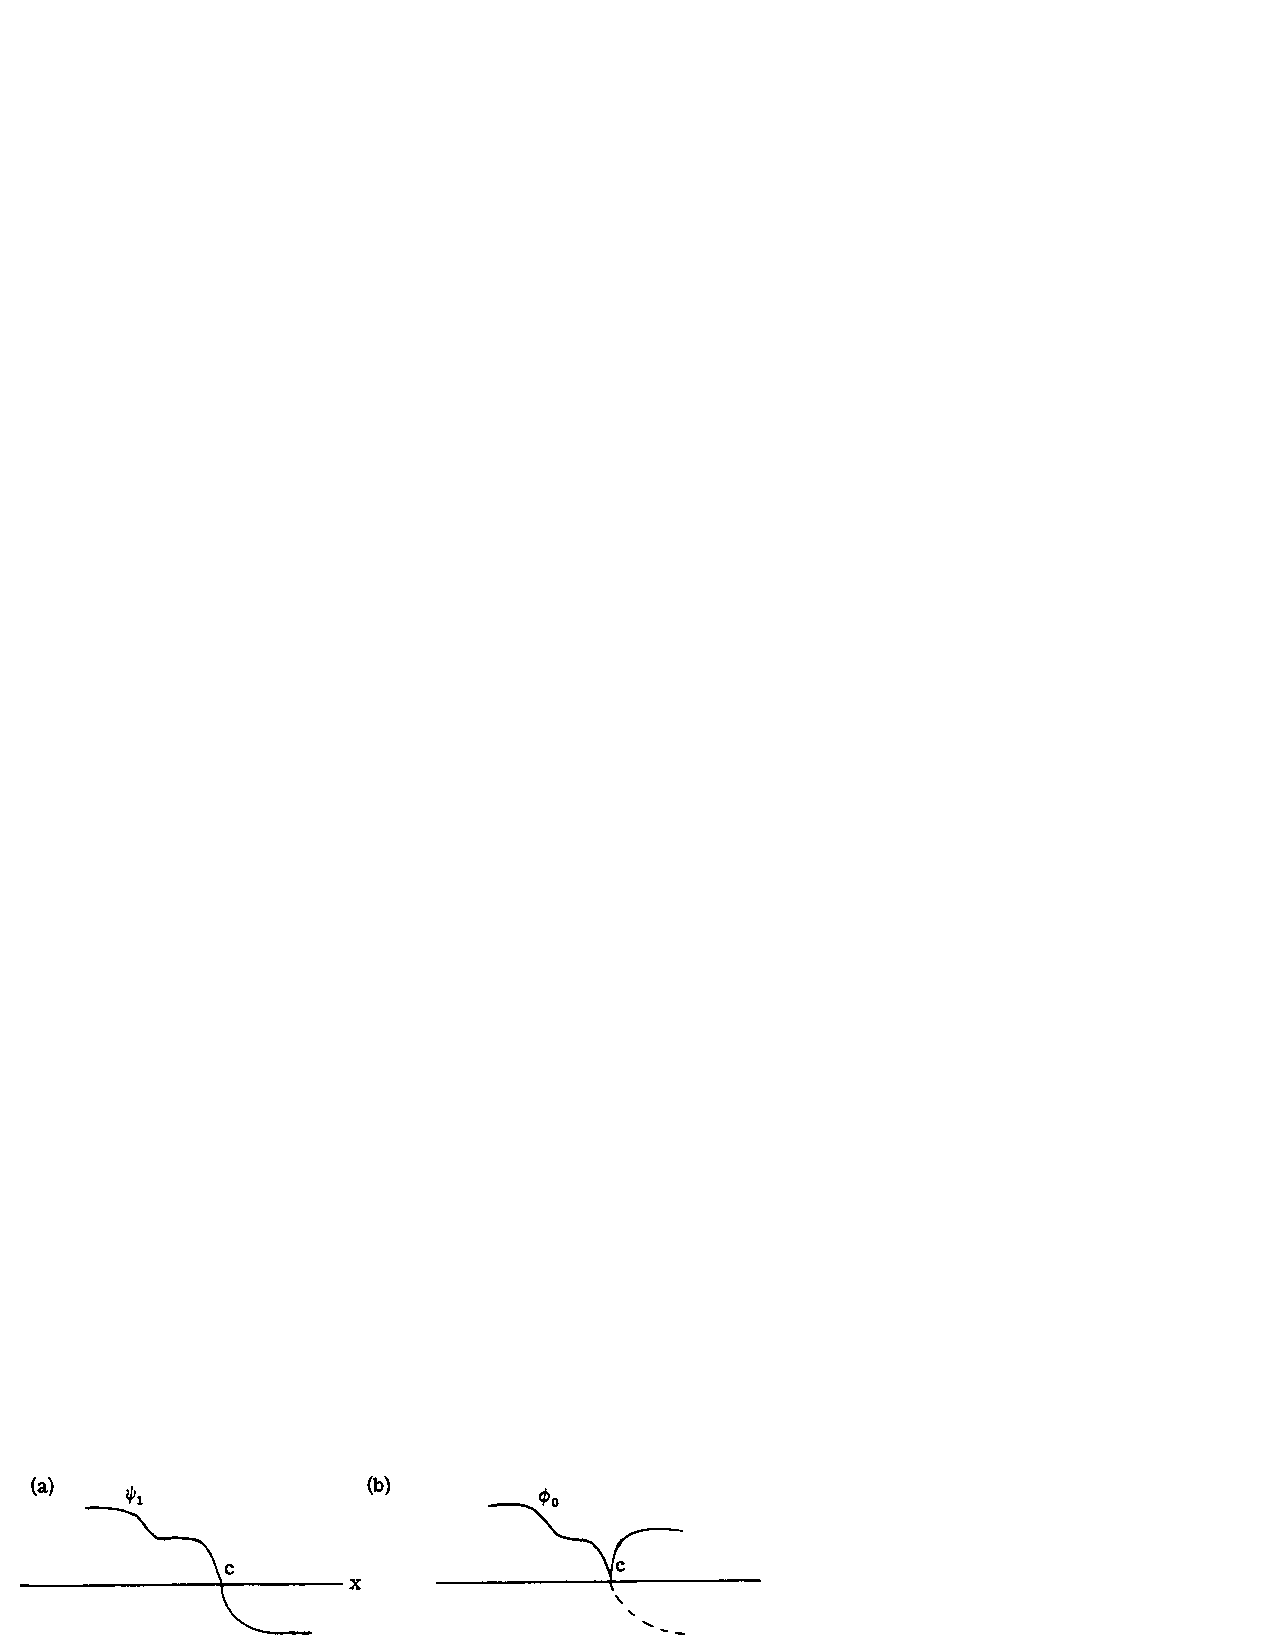
\includegraphics{fig1-10}
\caption{Illustration of the nodal theorem.}
\label{fig1-10}
\end{figure}

Consider first $\psi_1$, the lowest eigenstate of the Hamiltonian
\begin{equation}
{\hat H} \psi_1 = E_1 \psi_2
\end{equation}
having one sign change as in Figure \ref{fig1-10}(a).
From $\psi_1$ we can form a wavefunction $\varphi_0 = | \psi_1 |$, not
necessarily an eigenfunction of ${\hat H}$, that has no sign changes,
as in Figure \ref{fig1-10}(b). Since $\psi_1$ is normalized, then
$\varphi_0$ is also normalized,
\begin{equation}
\langle \varphi_0 \vert \varphi_0 \rangle = \int dx \vert \varphi_0 (x) \vert^2 = 
\int dx \vert \psi_1 ( x ) \vert^2 = 1,
\end{equation}
and the energy of $\varphi_0$ becomes
\begin{equation}
\epsilon_0 = \langle \varphi_0 \vert H \vert \varphi_0 \rangle = \langle \varphi_0 
\vert - {1 \over 2M} {d^2 \over dx^2} \vert \varphi_0 \rangle + \langle 
\varphi_0 \vert V \vert \varphi_0 \rangle.
\end{equation}
The potential energy of $\varphi_0$  is the same as that of $\psi_1$,

\begin{eqnarray}
\langle \varphi_0 \vert V \vert \varphi_0 \rangle 
                   &=& \int dxV(x) \vert \varphi_0(x)\vert^2\cr
                   &=& \int dxV(x) \vert \psi_1 (x) \vert^2\cr 
                   &=& \langle \psi_1 \vert V \vert \psi_1\rangle.
\label{eqno1-43}
\end{eqnarray}

From Section \ref{app-b}, the kinetic energy of $\psi_1$ can be expressed as
\begin{eqnarray}
\langle \psi_1 \vert - {1 \over 2m} {d^2 \over dx^2} \vert \psi_1 
\rangle &= {1 \over 2M} \langle \vert \triangle \psi_1 \vert^2 \rangle\cr
&= {1 \over 2M} \int^{+ \infty}_{- \infty} dx \vert {d \psi_1 \over dx} 
\vert^2\cr
\end{eqnarray}
But
\begin{equation}
{1 \over 2} \int^{- \infty}_{- \infty} dx \vert {d\psi_1 \over dx} 
\vert^2 = {1 \over 2} \int^{- \infty}_{- \infty} dx \vert {d \varphi_0 \over 
dx} \vert^2
\end{equation}
since the integrands are equal except at one point, $x_0$. Thus, the kinetic 
energies of $\varphi_0$ and $\psi_1$ are equal,
\begin{equation}
\langle \psi_1 \vert - {1 \over 2M} {d^2 \over dx^2} \vert \psi_1 
\rangle = \langle \varphi_0 \vert   - {1 \over 2M} {d^2 \over dx^2} \vert 
\varphi_0 \rangle ,\
\label{eqno1-44}
\end{equation}
and consequently from equations (\ref{eqno1-43}) and (\ref{eqno1-44})
the total energies of $\psi_1$ and $\varphi_0$ are equal,
\begin{equation}
\epsilon_0 = \langle \varphi_0 \vert H \vert \varphi_0 \rangle = \langle 
\psi_1 \vert H \vert \psi_1 \rangle = E_1.
\end{equation}
That is, given any eigenfunction $\psi_1$ of f${\hat H}$ that changes 
sign, we can construct a function $\varphi_0$
which does not change sign and yet has the same energy.
    
\begin{figure}
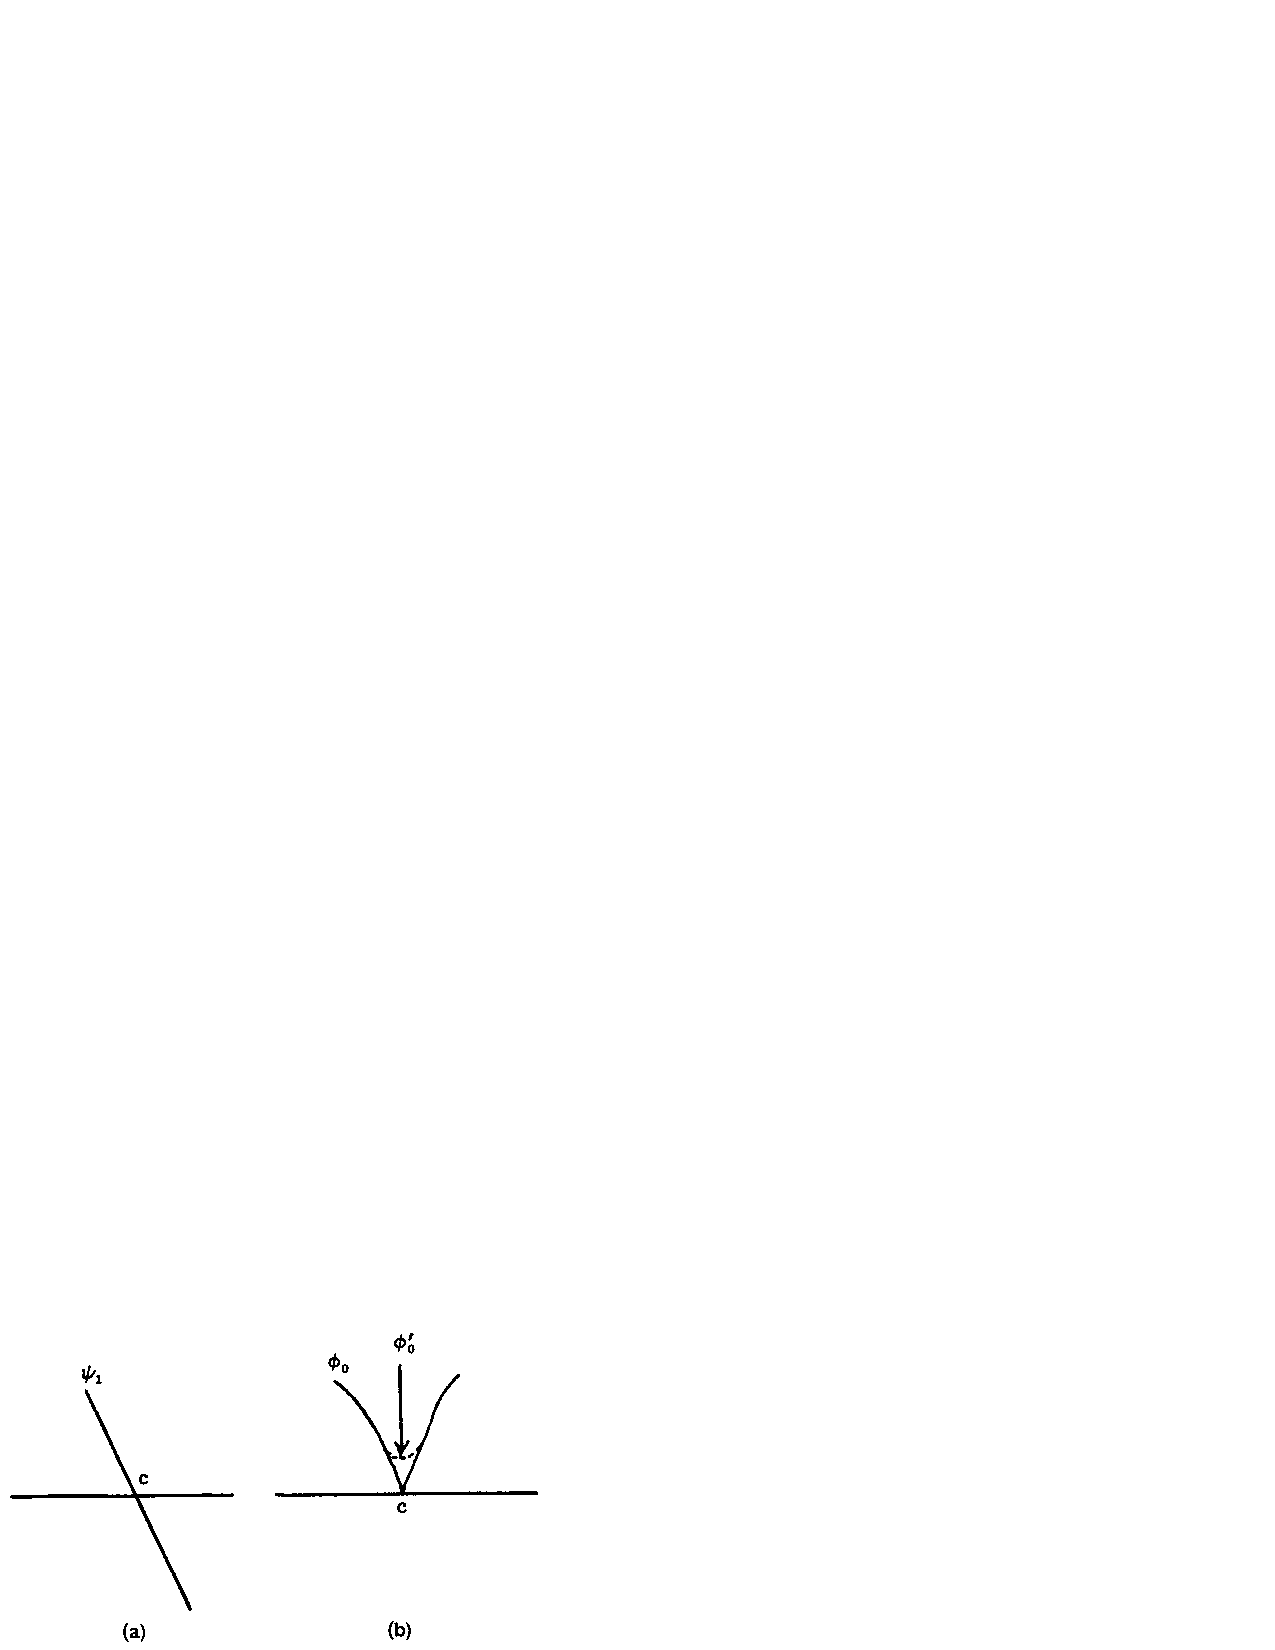
\includegraphics{fig1-11}
\caption{}
\label{fig1-11}
\end{figure}

Now consider a new function ${\bar \varphi}_0$ identical to $\varphi_0$ 
except that it is smoothed in the region very close to the position of the 
node $c$. If the potential is not singular at this point,
the function ${\bar \varphi}_0$ can be chosen to have the same potential 
energy, and normalization, as $\varphi_0$,
\begin{equation}
\langle {\bar \varphi}_0 \vert V \vert {\bar \varphi}_0 \rangle = \langle 
\varphi_0 \vert V \vert \varphi_0 \rangle.
\label{eq_hpp}
\end{equation}

However, since
\begin{equation}
\vert {d {\bar \varphi}_0 \over dx} \vert \ll \vert {d \varphi_0 \over dx} 
\vert
\end{equation}
in the region near $c$, $\varphi^{\prime}_0$ will have a smaller kinetic 
energy than $\varphi_0$,
\begin{equation}
{1 \over 2M} \langle \vert {d {\bar \varphi}_0 \over dx} \vert^2
\rangle < 
{1 \over 2M} \langle \vert {d \varphi_0 \over dx} \vert^2 \rangle.
\label{eq_1ov2m}
\end{equation}
Consequently, the energy of ${\bar \varphi}_0$ is lower than that of 
$\varphi_0$
\begin{equation}
{\bar \epsilon}_0 < \epsilon_0 = E_1.
\label{eq_eps0}
\end{equation}
The best, i.e., lowest energy, nodeless, i.e. non-negative, wavefunction has an
energy, $E_0$, no higher than ${\bar \epsilon}_0$, and hence, $E_0 < 
E_1$. Similar arguments can be used to derive the other relations. Thus, 
for a general potential we expect the bound solutions to increase in
the number of nodes as E increases, as in Figure \ref{fig1-12}.

\begin{figure}
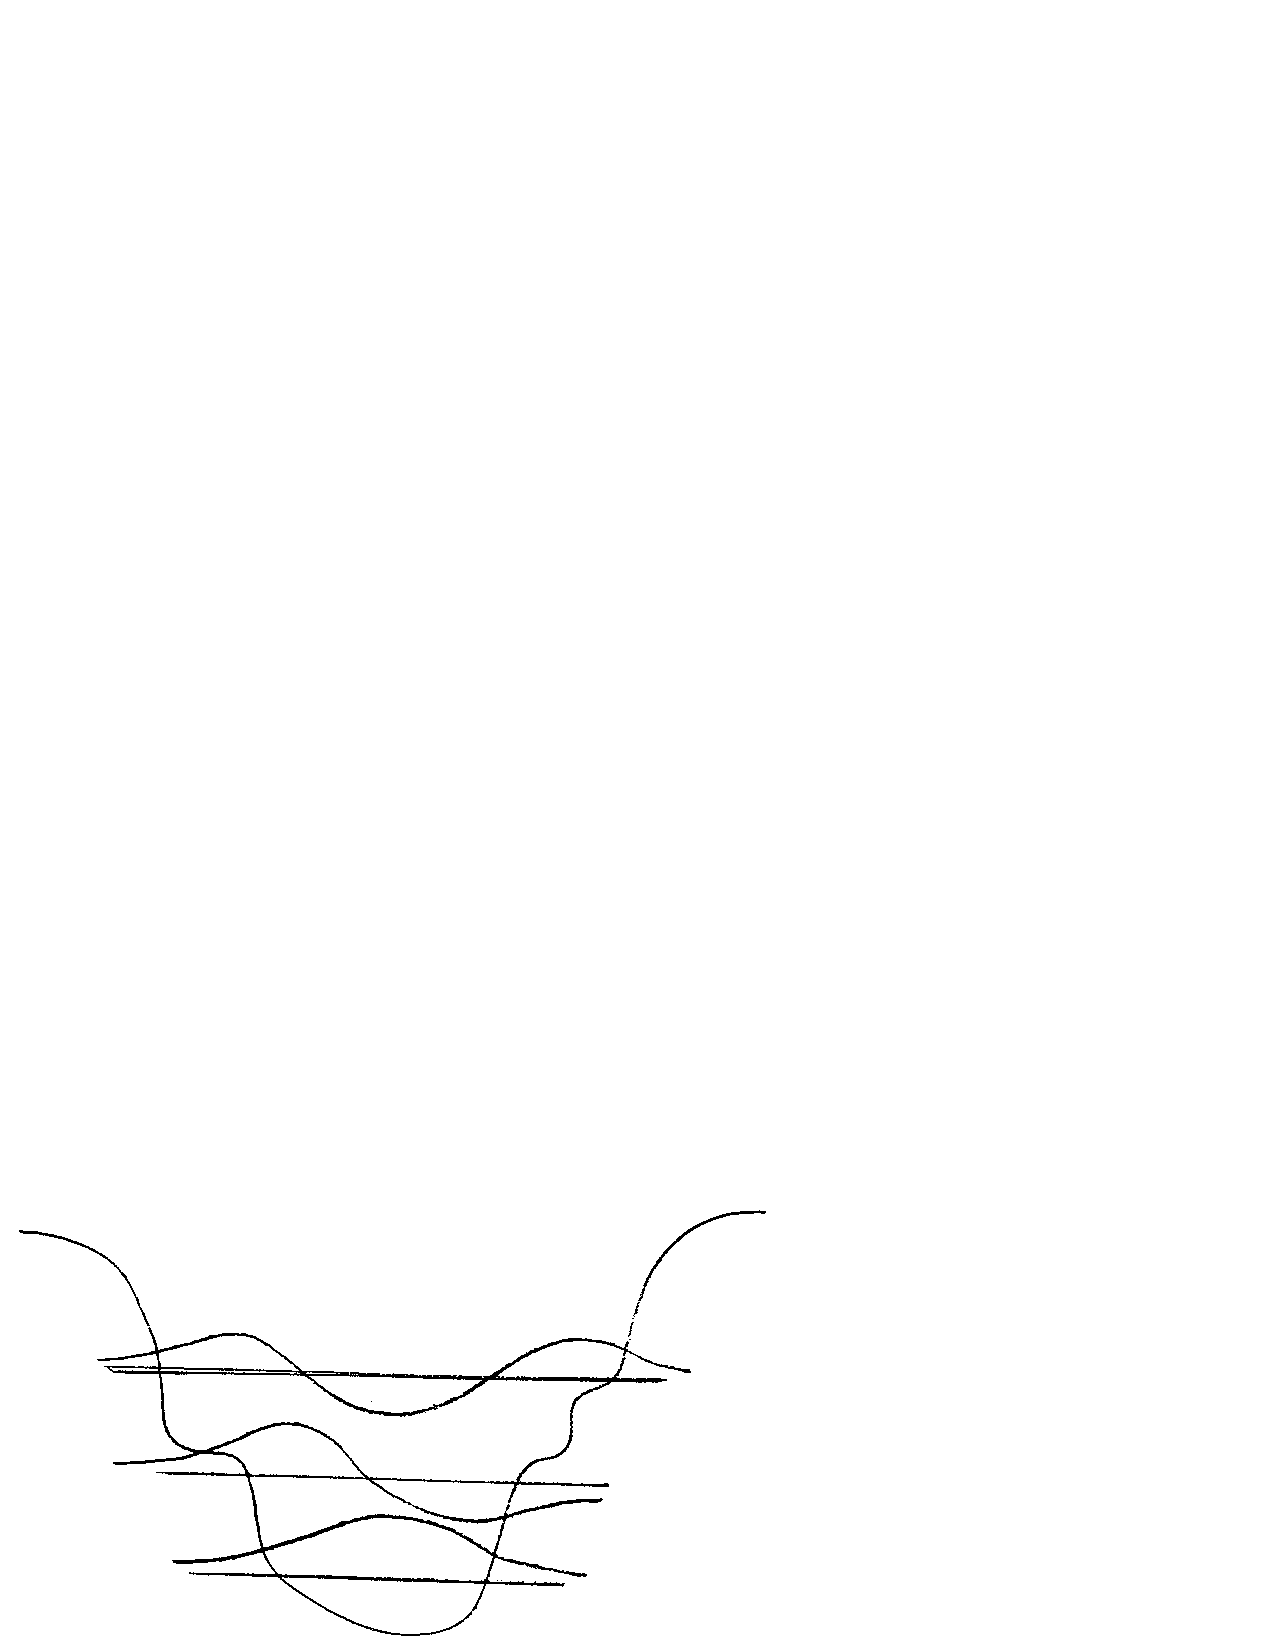
\includegraphics{fig1-12}
\caption{The nodal patterns of successive states of a general
(one-dimensional) potential.}
\label{fig1-12}
\end{figure}

\subsection{Multidimensions}
    
In two dimensions, a wavefunction that changes sign will have a line
of points with $\psi = 0$, a nodal line, and for three dimensions
there will be a surface of point with $\psi = 0$, a nodal surface. In
this section, we will use the same notation $nl$ as for states of the
three-dimensional $H$ atom. Just as in one dimension, the ground state
will always be nodeless. However, for multidimensions one can no
longer use the nodal theorem to order all states.  Thus, in two
dimension we can construct three orthogonal wavefunctions, all
orthogonal to the ground nodeless state, each with one nodal surface,
as illustrated in Figure \ref{fig1-13}.

\begin{figure}
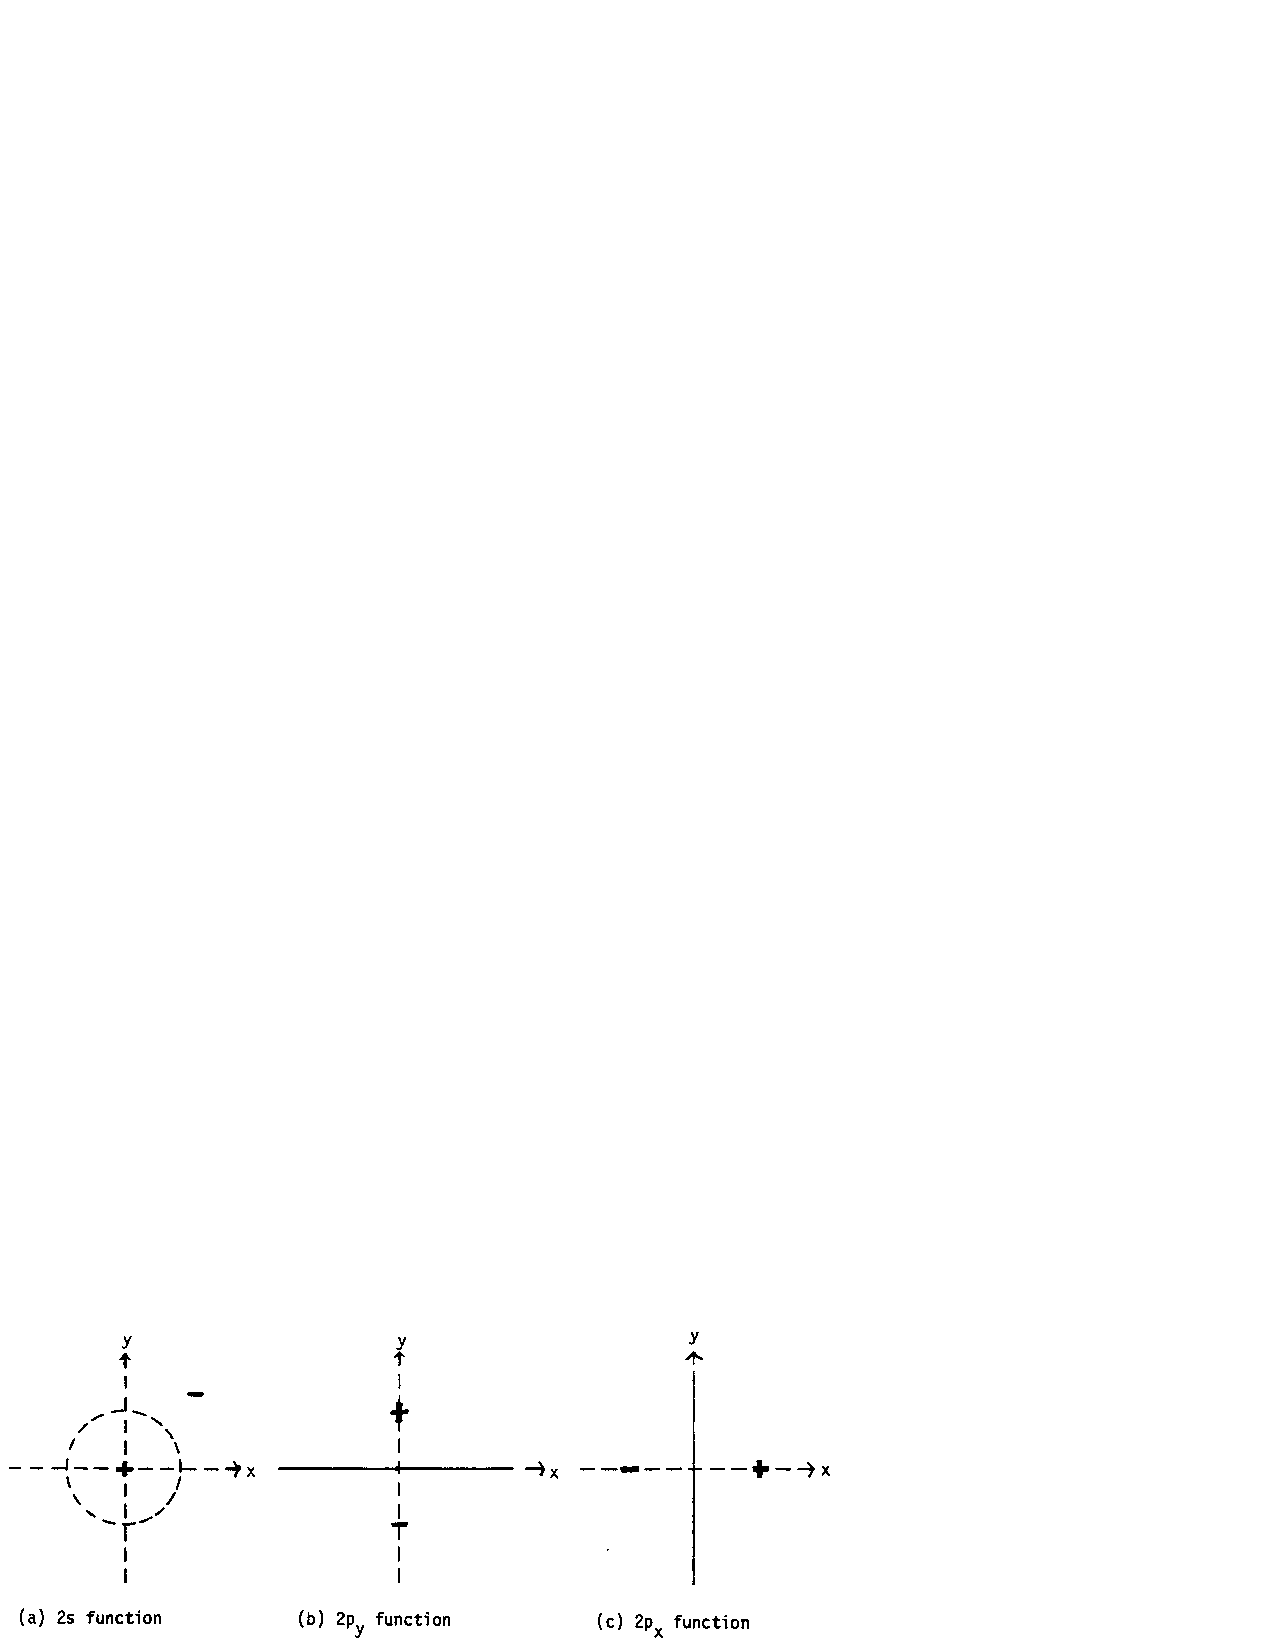
\includegraphics[scale=0.75]{fig1-13}
\caption{}
\label{fig1-13}
\end{figure}
    
If the potential energy is independent of angle, the wavefunctions in
Figure \ref{fig1-13}(b) and \ref{fig1-13}(c) will have the same
energy. However, the wavefunction in Figure \ref{fig1-13}(a) may be
higher, or lower, than the other two, depending on the exact form of
the potential. Even worse, we cannot use the nodal theorem to
determine whether the 3$s$ function in Figure \ref{fig1-14}(a) is above, or below,
the $2p$ functions of Figure \ref{fig1-13}(b) and \ref{fig1-13}(c).

\begin{figure}
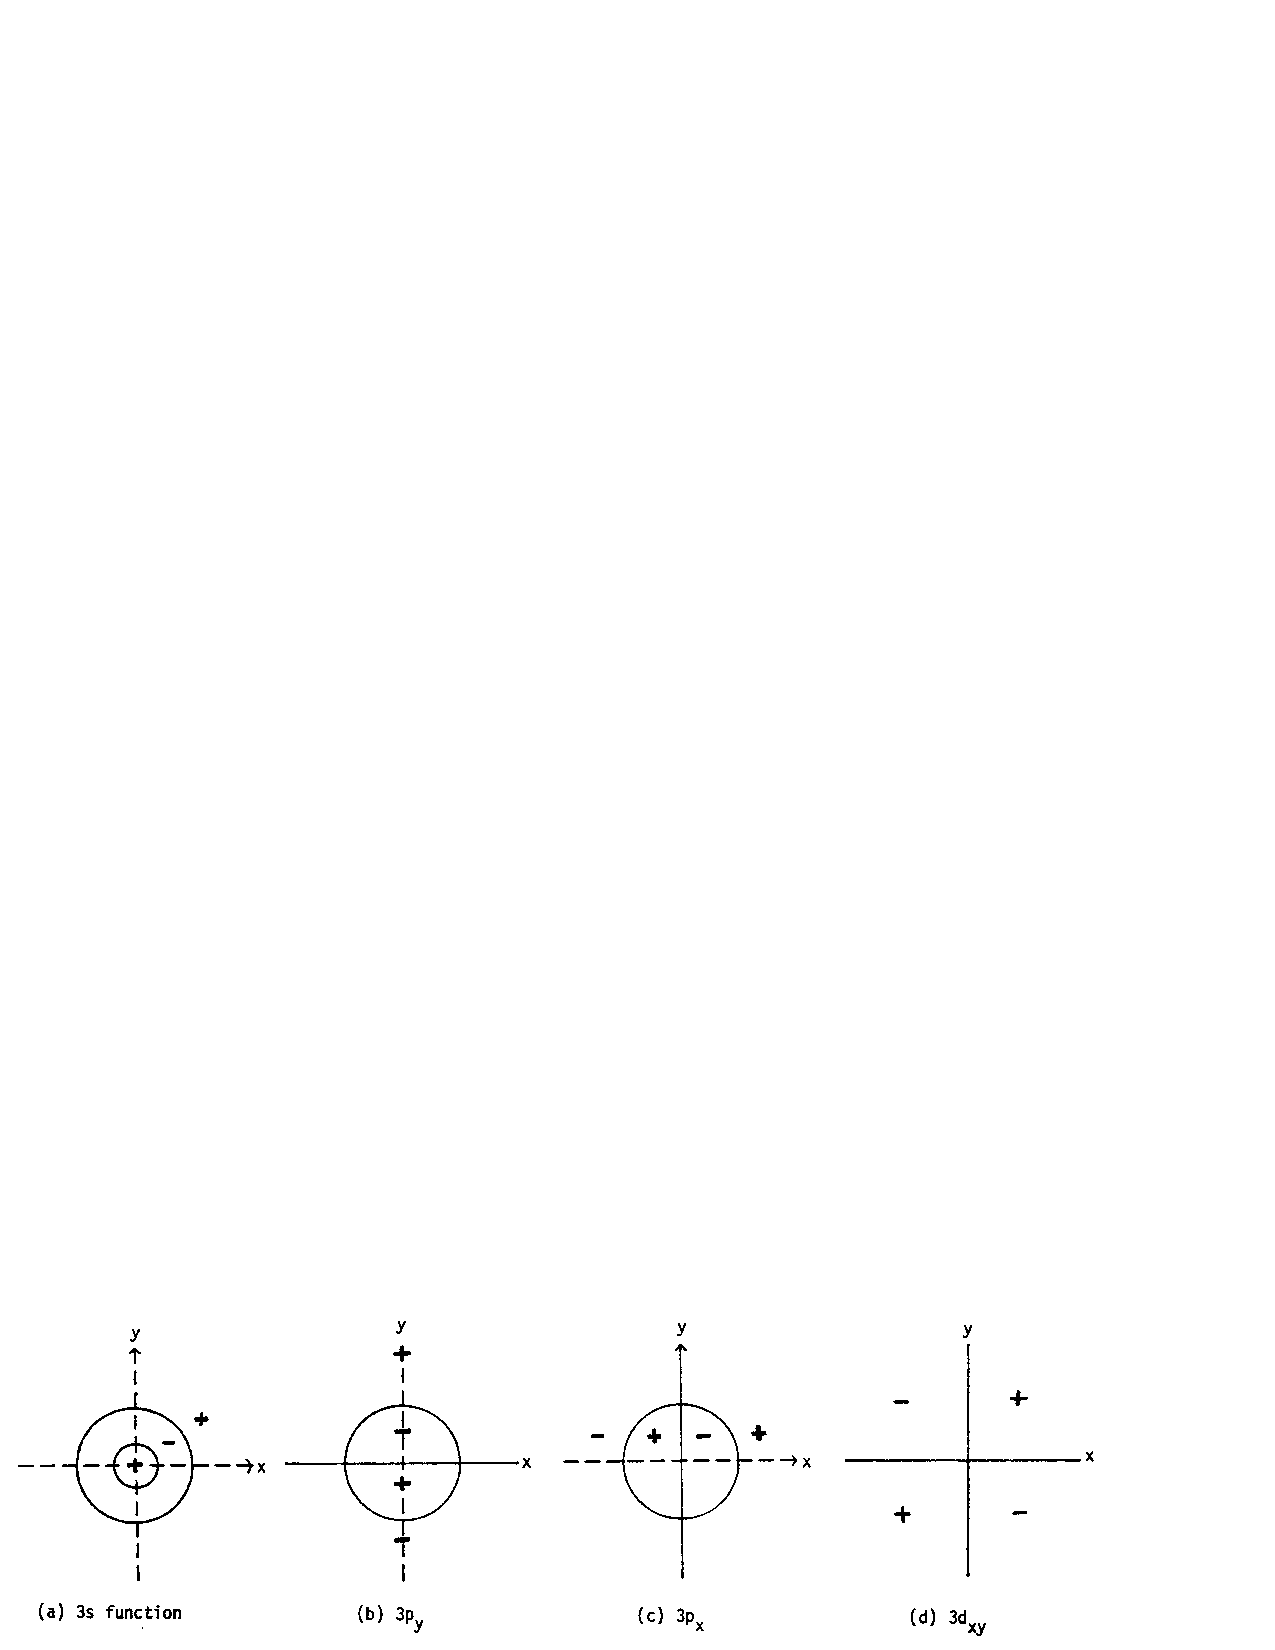
\includegraphics[scale=0.75]{fig1-14}
\caption{Two-Dimensional states with two nodal lines.}
\label{fig1-14}
\end{figure}

The clue to which comparisons can be made and which cannot is
apparent from the way that the one-dimensional theorem was proved in
the previous section.  Start with the optimum wavefunction of some
nodal structure, say Figure ???, and change the sign on opposite sides
of a single nodal surface to obtain either Figure \ref{fig1-15}(a) or
\ref{fig1-15}(b) by the same argument used in equations
\ref{eq_hpp}--\ref{eq_eps0}. The new wavefunctions in Figure
\ref{fig1-15}(a) and Figure \ref{fig1-15}(b) must have exactly the
same energy as Figure \ref{fig1-14}(c).

\begin{figure}
\begin{center}
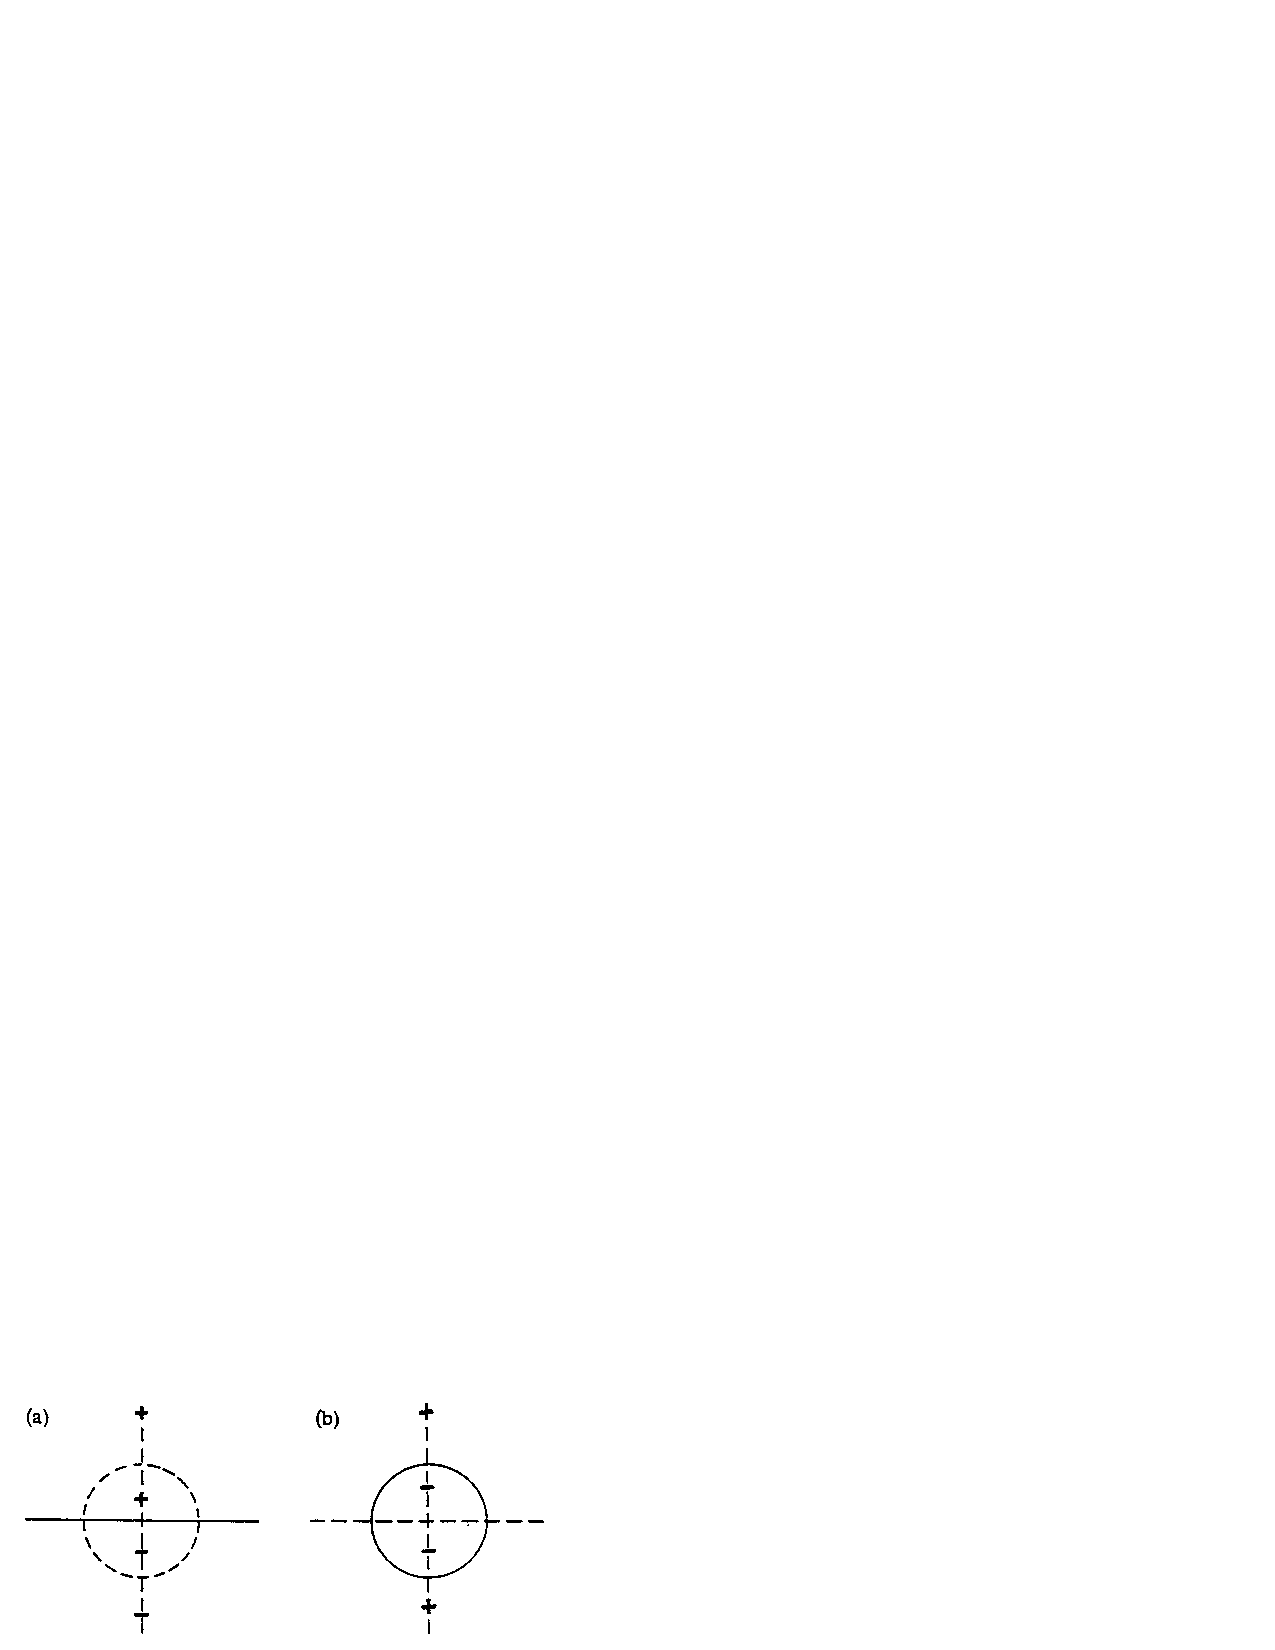
\includegraphics[scale=0.75]{fig1-15}
\end{center}
\caption{}
\label{fig1-15}
\end{figure}

The wavefunction in Figure \ref{fig1-15}(a) is an upper bound on the
$2p_y$ wavefunction of Figure \ref{fig1-13}(b). The wavefunction in
Figure \ref{fig1-15}(b) is an upper bound on the $2s$ wavefunction of
Figure \ref{fig1-13}(a).

\begin{figure}
\begin{center}
\begin{center}
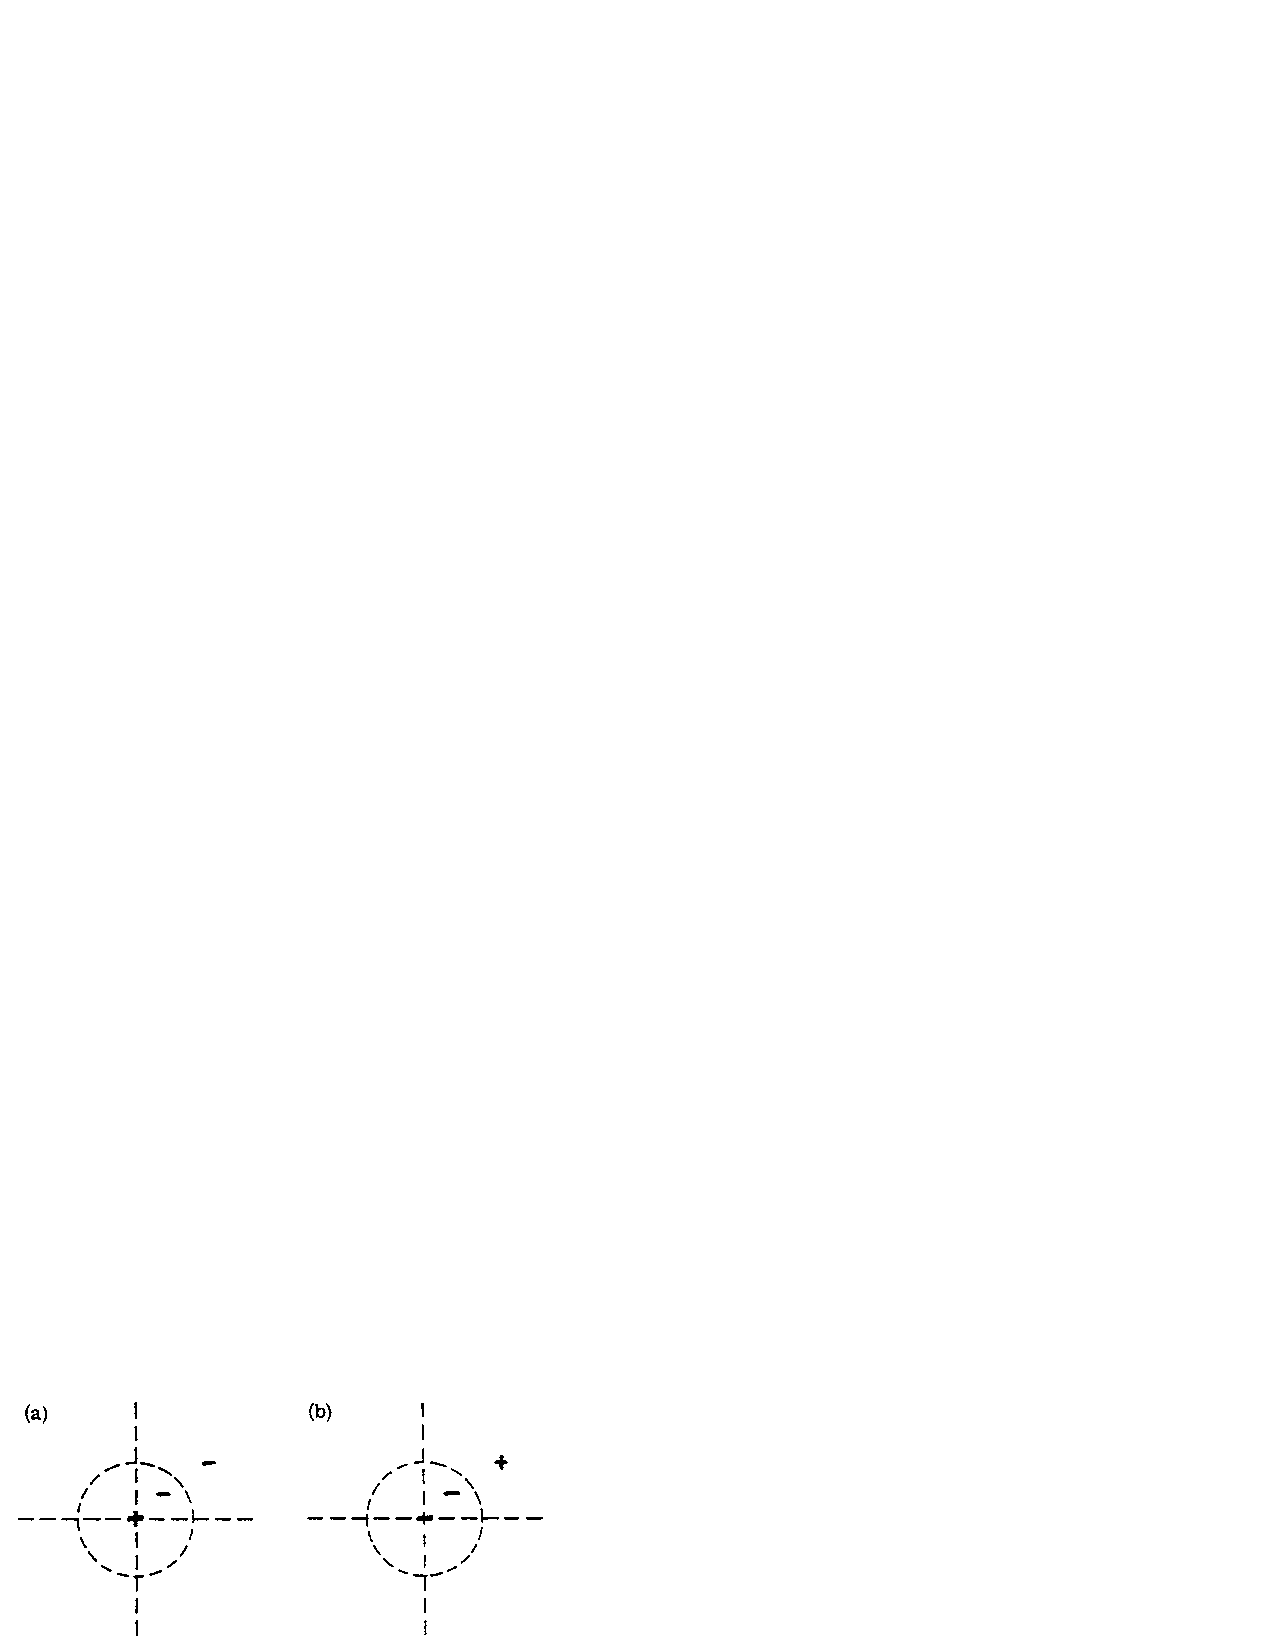
\includegraphics[scale=0.75]{fig1-16}
\end{center}
\end{center}
\caption{}
\label{fig1-16}
\end{figure}

Similarly, starting with the $3s$ wavefunction of Figure
\ref{fig1-14}(a), we see that the wavefunctions in Figure
\ref{fig1-16} have the same energy and are upper bounds to the $2s$
wavefunctions of Figure \ref{fig1-13}(a). However, there is no
wavefunction to compare the energy of the $3s$ wavefunctions with
those of the $2p$ wavefunctions. Continuing in this way, we can derive
the following relations,
$$
1s < 2s < 3s < 4s...
$$
$$
1s < 2p < 3p < 4p...
$$
$$
2s < 3p...
$$
$$
3s < 4p...
$$
$$
2p < 3d < 4d...
$$
$$
3p < 4d ... ,
$$
etc.

\section{Vibration and Rotation}
    
Throughout this course, we will focus upon the electronic wavefunctions for
molecules. Thus, for an $N$ electronic wavefunction, we determine 
$\Psi^{el}(1 , 2 , ... , N)$, with energy
\begin{equation}
E = {\langle \Psi^{el} \vert H \vert \Psi^{el} \rangle \over \langle \Psi^{cl} \vert 
\Psi^{el} \rangle},
\end{equation}
where ${\hat H}$ is the Hamiltonian for the system. The electronic 
wavefunction and its energy will depend upon the geometry of the molecule. For 
each geometry, we solve for the optimum wavefunction and energy at that 
geometry. For a diatomic molecule, the result is a total energy that is a 
function of $R$, internuclear distance, as indicated in Figure \ref{fig1-17}.

\begin{figure}
\begin{center}
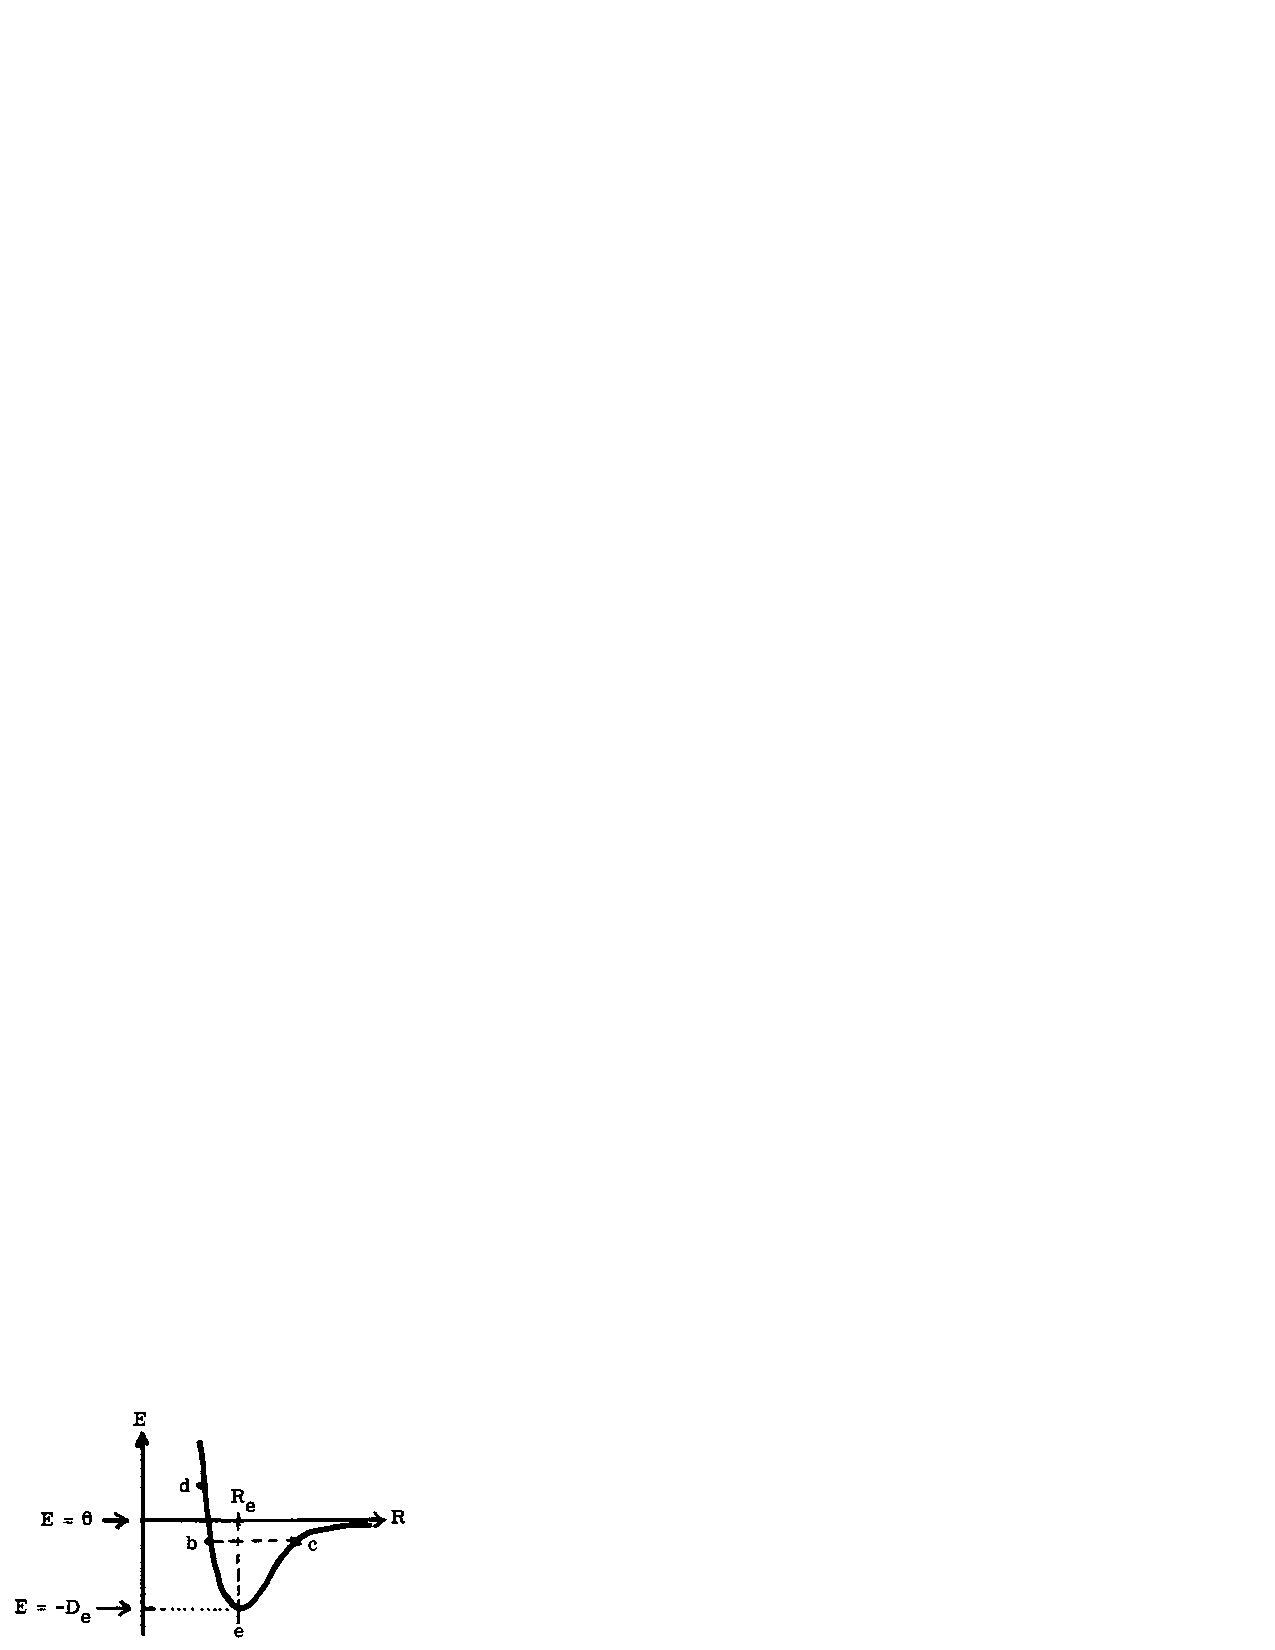
\includegraphics{fig1-17}
\end{center}
\caption{}
\label{fig1-17}
\end{figure}
    
As the nuclei move together, or move apart, we imagine the electrons
readjusting at each instant to reoptimize for that particular $R$. For
a classical system, if we started at some particular $R$, say point
$b$, the nuclei would move apart until they reached point $c$ and
would then come together until point $b$, and would continue
oscillating between these points, assuming no friction. Starting at
point $d$, the $R$ would continue increasing until $R = \infty$. On
the other hand, if we started at point $e$, the system would stay
still. Thus, point $e$ is called the equilibrium bond distance,
$R_e$. Starting with the molecule at equilibrium, $R_e$, the energy to
pull it apart, to break the bond, is called the bond energy, $D_e$.
    
\begin{figure}
\begin{center}
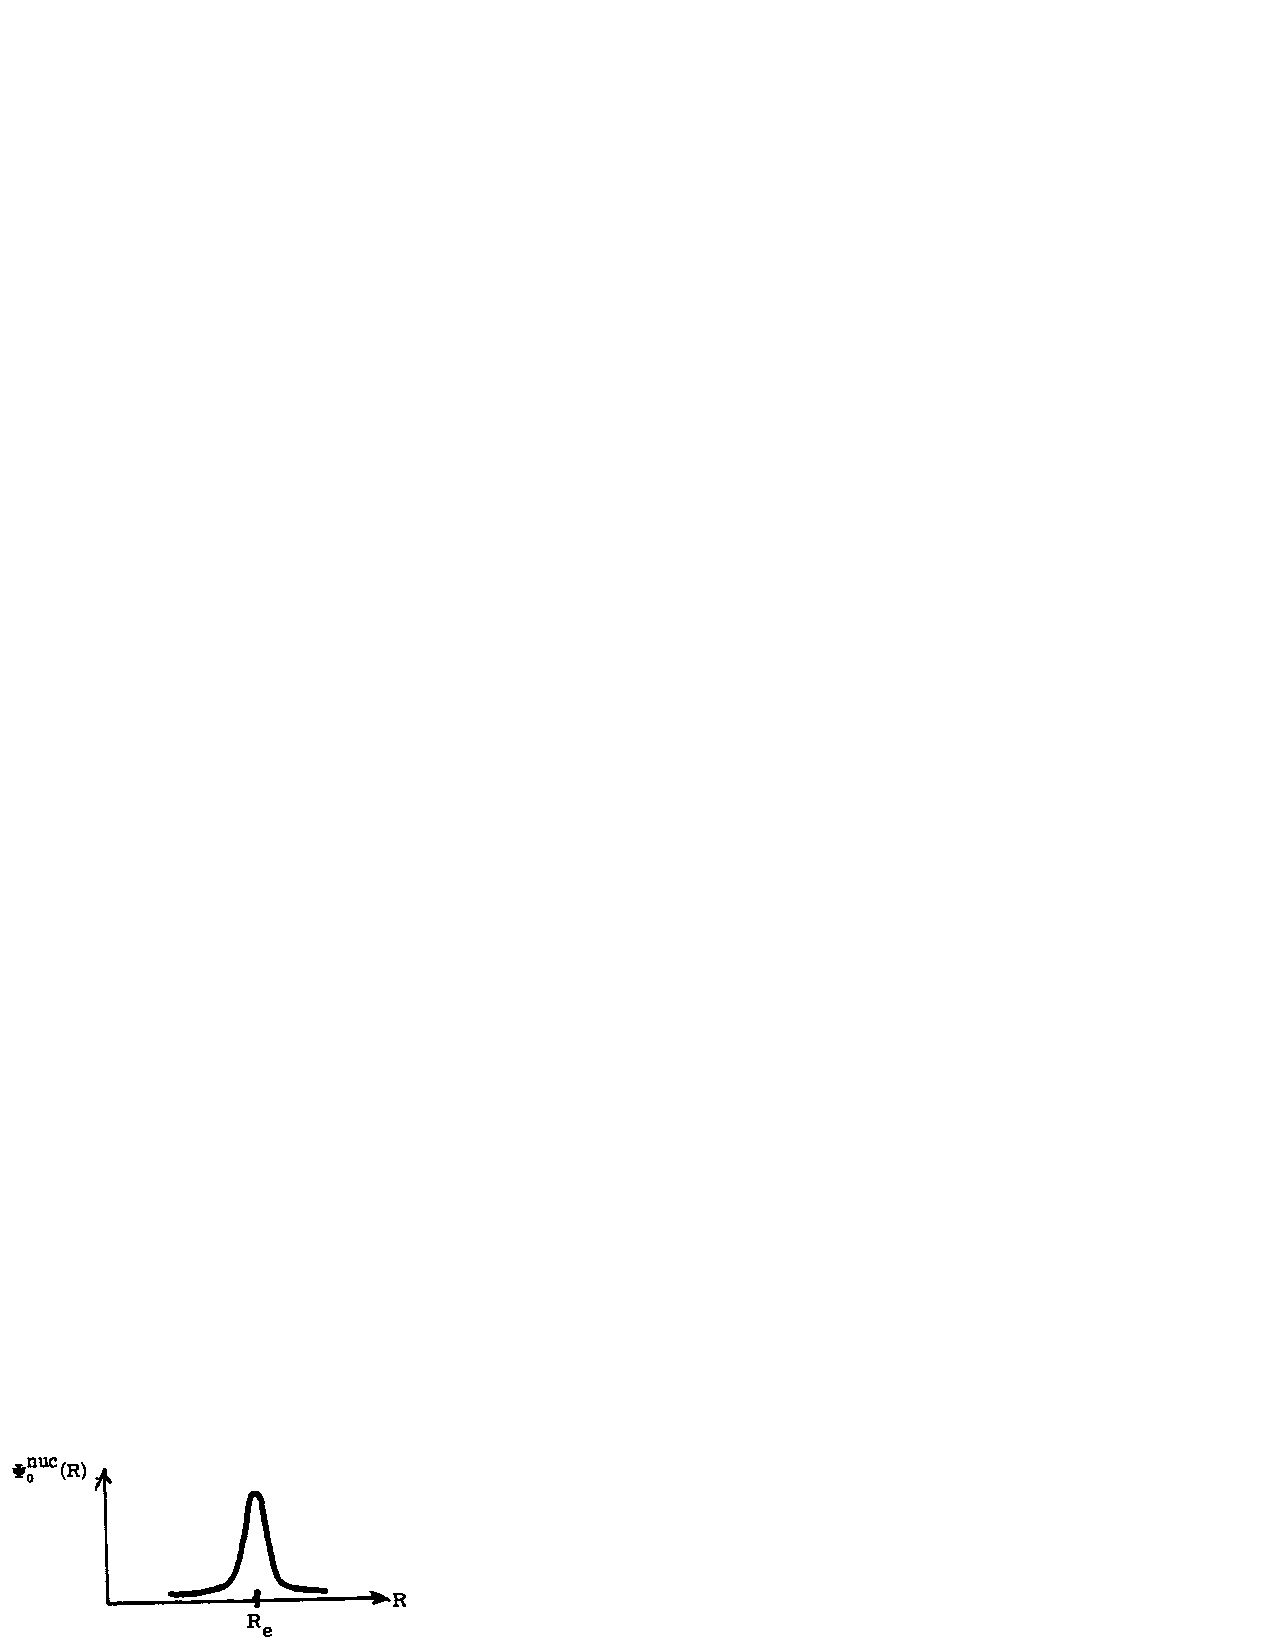
\includegraphics{fig1-18}
\end{center}
\caption{}
\label{fig1-18}
\end{figure}
    
For energies below the limit at infinity, we can think of the system
in terms of two masses, each corresponding to a proton, connected by a
spring of length $R_e$. However, in quantum mechanics, this spring can
never be completely at rest. The nuclear motions are described in
terms of wavefunctions, just as are the electrons, and the kinetic
energy of the nuclear motions depends on how localized the
wavefunctions are. To localize the nuclei at exactly $R = R_e$, would
imply an infinite kinetic energy. The result is that for the ground
state, the nuclear wavefunction has the form shown in Figure
\ref{fig1-18}.  That is, the most likely $R$ is $R_e$, but the nuclei
have a finite probability of being found at other $R$ near $R_e$. The
result is that the energy of the molecule is higher than the absolute
minimum, $E = -D_e$, in the energy curve by an amount referred to as
the zero-point energy. This lowest state, Figure \ref{fig1-18}, is
referred to as the ground vibrational state, $\Phi^{vib}$, with $v =
0$, and one thinks of the molecule as vibrating back and forth with a
frequency $\nu_0$.

At the bottom of a potential curve, the slope of the energy curve is
zero and the curvature is positive, so we can write
\begin{equation}
E(R) = E(R_e) + {1 \over 2} k(R - R_e)^2,
\end{equation}
where $k$, the curvature at the bottom of the well, is called the force constant
\begin{equation}
k = \left[ {\partial^2E \over \partial R^2} \right]_{R_e} .
\end{equation}
In this approximation, called the harmonic oscillator approximation, the
vibrational frequency is given by
\begin{equation}
\nu_0 = {1 \over 2 \pi} \sqrt{{k \over \mu}} ,
\end{equation}
where $\mu$ is the reduced mass
\begin{equation}
\mu = {M_1M_2 \over M_1+M_2}
\end{equation}
and $M_1$ and $M_2$ are the masses of the two nuclei. In this case, the 
zero-point energy is given by
\begin{equation}
{1 \over 2} \hbar \nu_0
\label{eqno1-45}
\end{equation}
where $h$ is Planck's constant. Thus, the energy of the ground vibrational 
state is $E = -D_0$, where
\begin{equation}
D_0 = D_e - {1 \over 2} h \nu_0 .
\end{equation}
The quantity $D_0$ is the actual energy to break the bond, starting with 
the molecule, in the ground vibrational state, and it is the quantity that 
would be measured experimentally.
    
In quantum mechanics, the excited vibrational wavefunctions must be orthogonal 
to the ground wavefunction, leading to the form in Figure \ref{fig1-19},

\begin{figure}
\begin{center}
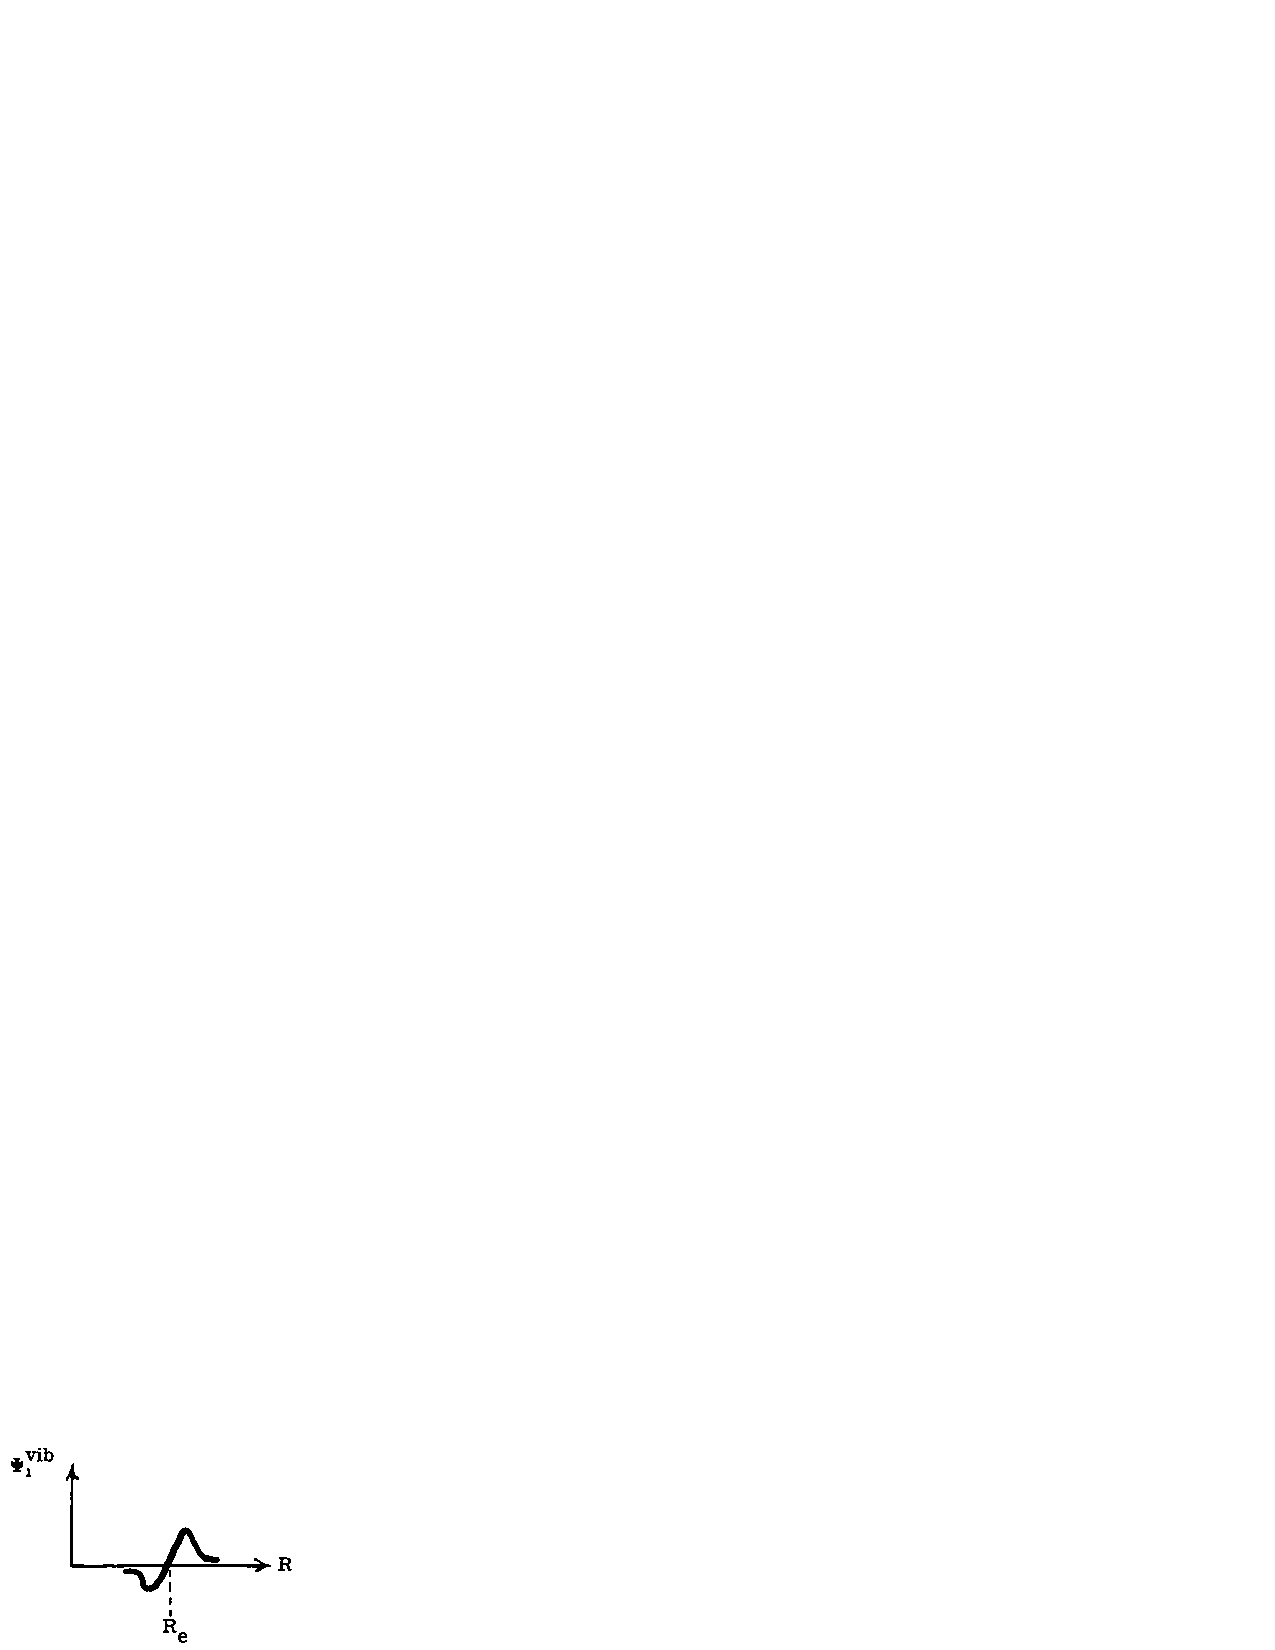
\includegraphics{fig1-19}
\end{center}
\caption{}
\label{fig1-19}
\end{figure}

\noindent
for the first excited vibrational state, $v = 1$. The excitation energy is
\begin{equation}
E_1 - E_0 = h \nu_0,
\label{eqno1-46}
\end{equation}
in the harmonic approximation. The separations between vibrational
states, as in equation (\ref{eqno1-46}), can be determined
experimentally, thereby providing experimental values for the
zero-point energy (\ref{eqno1-45}), and for the force constant $k$.
    
So far, we have considered the molecule to lie along the $z$ axis. In
fact, the axis of the molecule can be oriented along any direction in
space. Generally, the molecule will be rotating, but the ground
rotational state is the one for which all orientation are equally
likely. This is analogous to the $L = 0$, or $s$ state, for electrons
and is denoted as the $J = 0$ rotational state. Excited rotational
states have energies of
\begin{equation}
E_{rot} = {\hbar^2 \over 2I} J \left( J + 1 \right),
\end{equation}
where $I = \mu R^2_e$ is called the moment of inertia. This is analogous to the
classical rotational energy
\begin{equation}
E^{cl}_{rot} = {1 \over 2I} L^2 ,
\end{equation}
where $L$ is the rotational angular momentum. Experimentally, the bond distance of
molecules is often obtained by measuring the rotational energies and thereby deriving
$I$, and hence $R_e$.

For H$_2$ and H$^+_2$, the vibrational energies are $h \nu_0 =$ 4401
cm$^{-1}$ = 12.58 kcal/mol for H$_2$, and $h \nu_0 =$ 2322 cm$^{-1} =$
0.288 eV = 6.64 kcal/mol for H$^+_2$, and the rotational energies are
$E_j = BJ(J + 1)$, where $B =$ 60.85 cm$^{-1}$ for H$_2$, and $B =
$30.21 cm$^{-1}$ for H$^+_2$.  In these systems, the total bond
energies are $D_0 =$ 36117 cm$^{-1} =$ 4.478 eV = 103.3 kcal/mol for
H$_2$, and $D_0 =$ 21382 cm$^{-1} =$ 2.651 eV = 61.1 kcal/mol for
H$^+_2$.

\section{Appendices}
\subsection{Hermitian Operators}
\label{app-a}
    
In Section 1.2, we found that the basic postulate of quantum mechanics
implies that the wavefunction $\psi$ is normalized
\begin{equation}
\langle \psi \vert \psi \rangle = 1
\label{eqno1app-1}
\end{equation}
and that the time derivative of the wavefunction is determined by the relation
\begin{equation}
i \hbar {\partial \psi \over \partial t} = H \psi .
\label{eqno1app-2}
\end{equation}
Here we will show that these conditions imply that $H$ is a Hermitian operator
\begin{equation}
\langle \psi_j \vert H^{\dag} \vert \psi_k \rangle 
 = \langle \left( H \psi_j \right) \vert \psi_k \rangle 
 = \langle \psi_j \vert H \vert \psi_k \rangle
\end{equation}
for all allowed functions $\psi_j$ and $\psi_k$.  This property
results from the requirement that the total integrated probability
(\ref{eqno1app-1}) not change with time for any superposition of
allowed functions.

\subsubsection{Notation}

First we must established some notation. For any operator ${\hat B}$ and any
functions $\psi_j$ and $\psi_k$, we define the $jk$ matrix elements 
of ${\hat B}$ as
\begin{equation}
B_{jk} = \langle \psi_j \vert {\hat B} \vert \psi_k\rangle 
       = \int d \tau \psi_j ^* \left( {\hat B} \psi_k \right).
\label{eqno1app-3}
\end{equation}
The Hermitian conjugate of ${\hat B}$ is defined as the operator
${\hat B}^{\dag}$
\begin{equation}
\left( B^{\dag} \right)_{jk} = \langle \psi_j \vert {\hat B}^{\dag} \vert 
\psi_k \rangle = \int d \tau \left( {\hat B} \psi_j \right) ^* \psi_k = \langle 
\left( {\hat B} \psi_j \right) \vert \psi_k \rangle
\label{eqno1app-4}
\end{equation}
for all $\psi_j$ and $\psi_k$, of the Hilbert space. From equation
(\ref{eqno1app-3}) we see that
\begin{equation}
\langle \left( {\hat B} \psi_j \right) \vert \psi_k \rangle = \langle \psi_k \vert 
{\hat B} \psi_j \rangle ^* = B ^*_{ij},
\end{equation}
and hence, equation (\ref{eqno1app-4}) can be written
\begin{equation}
\left( B^{\dag} \right)_{jk} = B ^*_{kj}.
\end{equation}
If ${\hat B}$ is equal to its Hermitian conjugate,
\begin{equation}
\langle \psi_j \vert {\hat B}^{\dag} \vert \psi_k \rangle = \langle \psi_i \vert B 
\vert \psi_k \rangle ,
\end{equation}
we say that ${\hat B}$ is Hermitian and write
\begin{equation}
{\hat B}^{\dag} = {\hat B} .
\end{equation}

\subsubsection{Hermitivity of $\hat{H}$}
    
From equation (\ref{eqno1app-1}) the total probability of finding the
partial somewhere, $\langle \psi \vert \psi\rangle = 1$, is independent of
time. Thus, taking the derivative with respect to time, we have
\begin{equation}
0 = \langle {\partial \psi \over \partial t} \vert \psi \rangle + \langle 
\psi \vert {\partial \psi \over \partial t} \rangle = \int d \tau 
\left[ {\partial \psi ^* \over \partial t} \psi + \psi ^* {\partial 
\psi \over \partial t} \right] .
\end{equation}
Substituting the Schr\"odinger equation (\ref{eqno1app-2}) here, leads to
\begin{equation}
0 = \left( i \hbar \right)^{-1} \int d \tau \left[ \left( - H \psi \right) ^* 
\psi + \psi ^* ( \psi ) \right]
\end{equation}
or
\begin{equation}
0 = \left\{ - \langle \psi \vert H \vert \psi \rangle ^* + \langle
\psi \vert H \vert \psi \rangle \right\} ,
\end{equation}
which implies that the quantity $E \equiv \langle \psi \vert H \vert 
\psi \rangle$, referred to as the energy, is real.
    
Consider, now, the superposition
\begin{equation}
\psi = C_j \psi_j + C_k \psi_k
\end{equation}
where $C_j$ and $C_k$ are numbers, possibly complex, of two states 
$\psi_j$ and $\psi_k$ that are orthogonal
\begin{equation}
\langle \psi_j \vert \psi_k \rangle = 0
\end{equation}
at some time $t_0$. Then since $ \langle \psi \vert \psi\rangle$,
$\langle \psi_j \vert \psi_j \rangle$, and $\langle \psi_k \vert
\psi_k \rangle$ are all unity and independent of time, it must be that
\begin{equation}
C ^*_k  C_j \langle \psi_k \vert \psi_j\rangle 
+ C ^*_j C_k \langle \psi_j \vert \psi_k \rangle 
= \langle \psi \vert \psi \rangle
- C ^*_j C_j \langle \psi_j \vert \psi_j \rangle 
- C ^*_k C_k \langle \psi_k \vert \psi_k \rangle
\label{eqno1app-5a}
\end{equation}
is also independent of time.  Simiarly, considering
\begin{equation}
\psi^{\prime} = i C_j \psi_j + C_k \psi_k
\end{equation}
where $i = \sqrt{-1}$, we find that for $\langle \psi^{\prime} \vert 
\psi^{\prime} \rangle$ to be independent of time, requires that
\begin{equation}
iC_k ^* C_j \langle \psi_k \vert \psi_j \rangle - iC_j ^* C_k \langle \psi_j \vert 
\psi_k \rangle
\label{eqno1app-5b}
\end{equation}
also be independent of time. Combining equations
(\ref{eqno1app-5a})and (\ref{eqno1app-5b}), leads to the condition that
\begin{equation}
\langle \psi_j \vert \psi_k \rangle = 0
\end{equation}
is independent of time. This leads to
\begin{equation}
0 = \langle {\partial \psi_j \over \partial t} \vert \psi_k \rangle + 
\langle \psi_j \vert {\partial \psi_k \over \partial t} \rangle = i 
\hbar \left[ - \langle \psi_j \vert {\hat H}^{\dag} \vert \psi_k \rangle + \langle 
\psi_j \vert {\hat H} \vert \psi_j \rangle \right],
\end{equation}
and hence
\begin{equation}
\langle \psi_j \vert {\hat H} \psi_k \rangle = \langle \psi_j \vert {\hat H}^{\dag} 
\vert \psi_k \rangle
\label{eqno1app-6}
\end{equation}
which also applies to $j = k$.  The relation (\ref{eqno1app-6}) must
apply to all possible pairs of functions $\psi_j$ and $\psi_k$, and
hence, the Hamiltonian operator, $H$, must be a Hermitian
operator. From this derivation we see that the Hermitian property of
${\hat H}$ results from the assumption that the total integrated
probability of any superposition of functions is independent of time,
conservation of normalization.

\subsubsection{The Momentum Operator}
    
An example is appropriate here. Consider a one-dimensional system with coordinates
in the range $0 \leq x \leq a$. Is the operator
\begin{equation}
{\hat p} = {\hbar \over i} {d \over dx}
\end{equation}
Hermitian? To find out, we consider
\begin{equation}
 \langle\psi_j\vert{\hat p}^{\dag}\vert\psi_k\rangle 
   = - {\hbar \over i} 
      [\psi_j^*(a)\psi_k(a)-\psi_j^*(0)\psi_k(0)]
 + {\hbar\over i}\int^{a}_{0} dx\psi_j^*{d\psi_k\over dx}
\end{equation}
or 
\begin{equation}
\langle \psi_j \vert {\hat p}^{\dag} \vert \psi_k \rangle = - {\hbar \over i} 
\left[ \psi ^*_j (a) \psi_k (a) - \psi ^*_j (0) \psi_k (0) \right] + \langle 
\psi_j \vert {\hat p} \vert \psi_k \rangle
\end{equation}
Thus, the operator ${\hat p}$ is Hermitian if, and only if, the boundary 
conditions axe such that
\begin{equation}
\psi ^*_j (a) \psi_k (a) = \psi ^*_j (0) \psi_k (0)
\end{equation}
for all allowed functions $\psi_j$ and $\psi_k$. Thus, it is nonsense to say the
\begin{equation}
{\hat p} = {\hbar \over i} {d \over dx}
\end{equation}
is an Hermitian operator; rather, one must say that the operator is Hermitian given
such, and such boundary conditions. Some acceptable boundary conditions, for the
above case, are, first that $\psi (A) = 0$ and $\psi (0) = 0$ which is the case of 
a particle in a box. Secondly, $\psi (a) = \psi (0)$ which corresponds to 
periodic boundary conditions here the point $x = a$ is physically equivalent 
to the point $x = 0$.  A common example is for angular coordinate 
$\varphi$ where $a = 2 \pi$ is identically the same point as $x = 
0$.  And finally, for systems of infinite range $- \infty < x < + 
\infty$, then for $\varphi$ to be normalized, $ \langle \varphi \vert 
\varphi \rangle = 1$, it must be that $\varphi \rightarrow 0$ as $x 
\rightarrow \pm \infty$, leading to $\varphi_j ^* (a) \varphi_k (a) 
\rightarrow 0$ as $a \rightarrow \pm \infty$. 

If the boundary conditions are such that $\hat p$ is Hermitian, then the kinetic 
energy operator
\begin{equation}
T = {1 \over 2m} {\hat p}^2
\end{equation}
is necessarily Hermitian. This follows by applying the Hermitian properties
of $p$ sequentially,
\begin{equation}
\langle \left( {\hat p}_x {\hat p}_x \psi_j \right) \vert \psi_k \rangle = \langle 
\left( {\hat p}_x \psi_j \right) \vert {\hat p}_x \vert \psi_k \rangle = \langle 
\psi_j \vert {\hat p}_x {\hat p}_x \psi_k \rangle .
\end{equation}

\subsection{The Kinetic Energy}
\label{app-b}

In this section, we will show that the matrix element
\begin{equation}
t_{ab} = \langle \varphi_a \vert - {1 \over 2} \nabla^2 \vert
\varphi_b\rangle
\label{eqno1app-7}
\end{equation}
can be written as
\begin{equation}
t_{ab} = {1 \over 2} \langle \nabla \varphi_a \cdot \nabla \varphi_b \rangle ,
\end{equation}
where the dot product is indicated. Thus, the kinetic energy of an orbital
becomes
\begin{equation}
t_{aa} = {1 \over 2} \langle \vert \nabla \varphi_a \vert^2 \rangle
\label{eqno1app-8a}
\end{equation}
in atomic units, or
\begin{equation}
t_{aa} = {\hbar^2 \over 2m} \langle \vert \nabla \varphi_a \vert^2 
\rangle
\label{eqno1app-8b}
\end{equation}
in other units.

Consider first the integral
\begin{equation}
\langle \varphi_a \vert {\partial^2 \over \partial x^2} \vert 
\varphi_b \rangle - \int \int \int^{+ \infty}_{- \infty} d x d y d x 
\varphi ^*_a {\partial^2 \varphi_b \over \partial x^2}.
\end{equation}
Integrating by parts, this becomes
\begin{equation}
Q(x = + \infty ) - Q ( x = - \infty) - \int \int \int^{+ \infty}_{- 
\infty} d x d y d z {\partial \varphi^*_a \over \partial x} {\partial 
\varphi_b \over \partial x},
\end{equation}
where
\begin{equation}
Q = \int \int^{+ \infty}_{- \infty} d y d z \varphi ^*_a {\partial 
\varphi^*_b \over \partial x}
\end{equation}
this is referred to as Green's theorem.  However, for $\varphi_a$ and 
$\varphi_b$ to satisfy the basic postulates of quantum mechanics, we must 
have $ \langle \varphi_a | \varphi_a \rangle = 1$, $\langle \varphi_b | \varphi_b = 1$, 
and hence $\varphi_a \rightarrow 0$ as $x \rightarrow \pm \infty$.  
Thus, $Q ( x = + \infty) = 0$ and $Q ( x = - \infty) = 0$ we obtain
\begin{equation}
\langle \varphi_a \vert {\partial^2 \over \partial x^2} \vert 
\varphi_b \rangle = - \langle {\partial \varphi_a \over \partial_x} 
\vert {\partial \varphi_b \over \partial x} \vert \rangle .
\end{equation}
Proceeding similarly for the other terms of equation
(\ref{eqno1app-7}), we obtain
\begin{equation}
t_{ab} = {1 \over 2} \int d \tau \left[ \nabla \varphi ^*_a \nabla 
\varphi_b \right] \equiv {1 \over 2} \langle \nabla \varphi_a \cdot \nabla 
\varphi_b \rangle ,
\end{equation}
and letting $\varphi_a = \varphi_b$, leads to equations
(\ref{eqno1app-8a})--(\ref{eqno1app-8b}).

\subsection{The Nodal Theorem}
\label{app-c}
    
In this section, we consider the eigenfunctions $\varphi_n$ for a general 
one-dimensional system, $H \varphi_n = E_n \varphi_n$, where
\begin{equation}
H = - {1 \over 2M} {d^2 \over dx^2} + V (x)
\end{equation}
is real, so that the eigenfunctions are real, and
\begin{equation}
M = {m \over \hbar^2}.
\end{equation}

Letting $n$ denote the number of nodes, internal to the boundaries, we will 
show that
\begin{equation}
E_0 < E_n
\label{eqno1app-9}
\end{equation}
and
\begin{equation}
E_n < E_{n+1} .
\label{eqno1app-10}
\end{equation}
That is, the ground state of the system is nodeless and the state with
$n$ nodes has a lower energy than the state with $n + 1$ nodes. For
sufficiently singular potentials, the inequalities in equations
(\ref{eqno1app-9}) and (\ref{eqno1app-10}) become equalities.

\subsubsection{The Inequalities}

Consider first the functions $\varphi_0$ and $\varphi_1$, which are the 
eigenstates of ${\hat H}$,
\begin{eqnarray}
{\hat H} \varphi_0 &= \left( {\hat T} + {\hat V} \right) \varphi_0 = E_0 
\varphi_0\cr
{\hat H} \varphi_1 &= \left( {\hat T} + {\hat V} \right) \varphi_1 = E_1 
\varphi_1,\cr
\label{eqno1app-11}
\end{eqnarray}

with zero and one node, respectively, as in Figure \ref{fig1-20}. Here $a$ and 
$b$ are the boundaries of the system, they may be at $\pm \infty$, and 
zeroes at the boundaries are not counted.

\begin{figure}
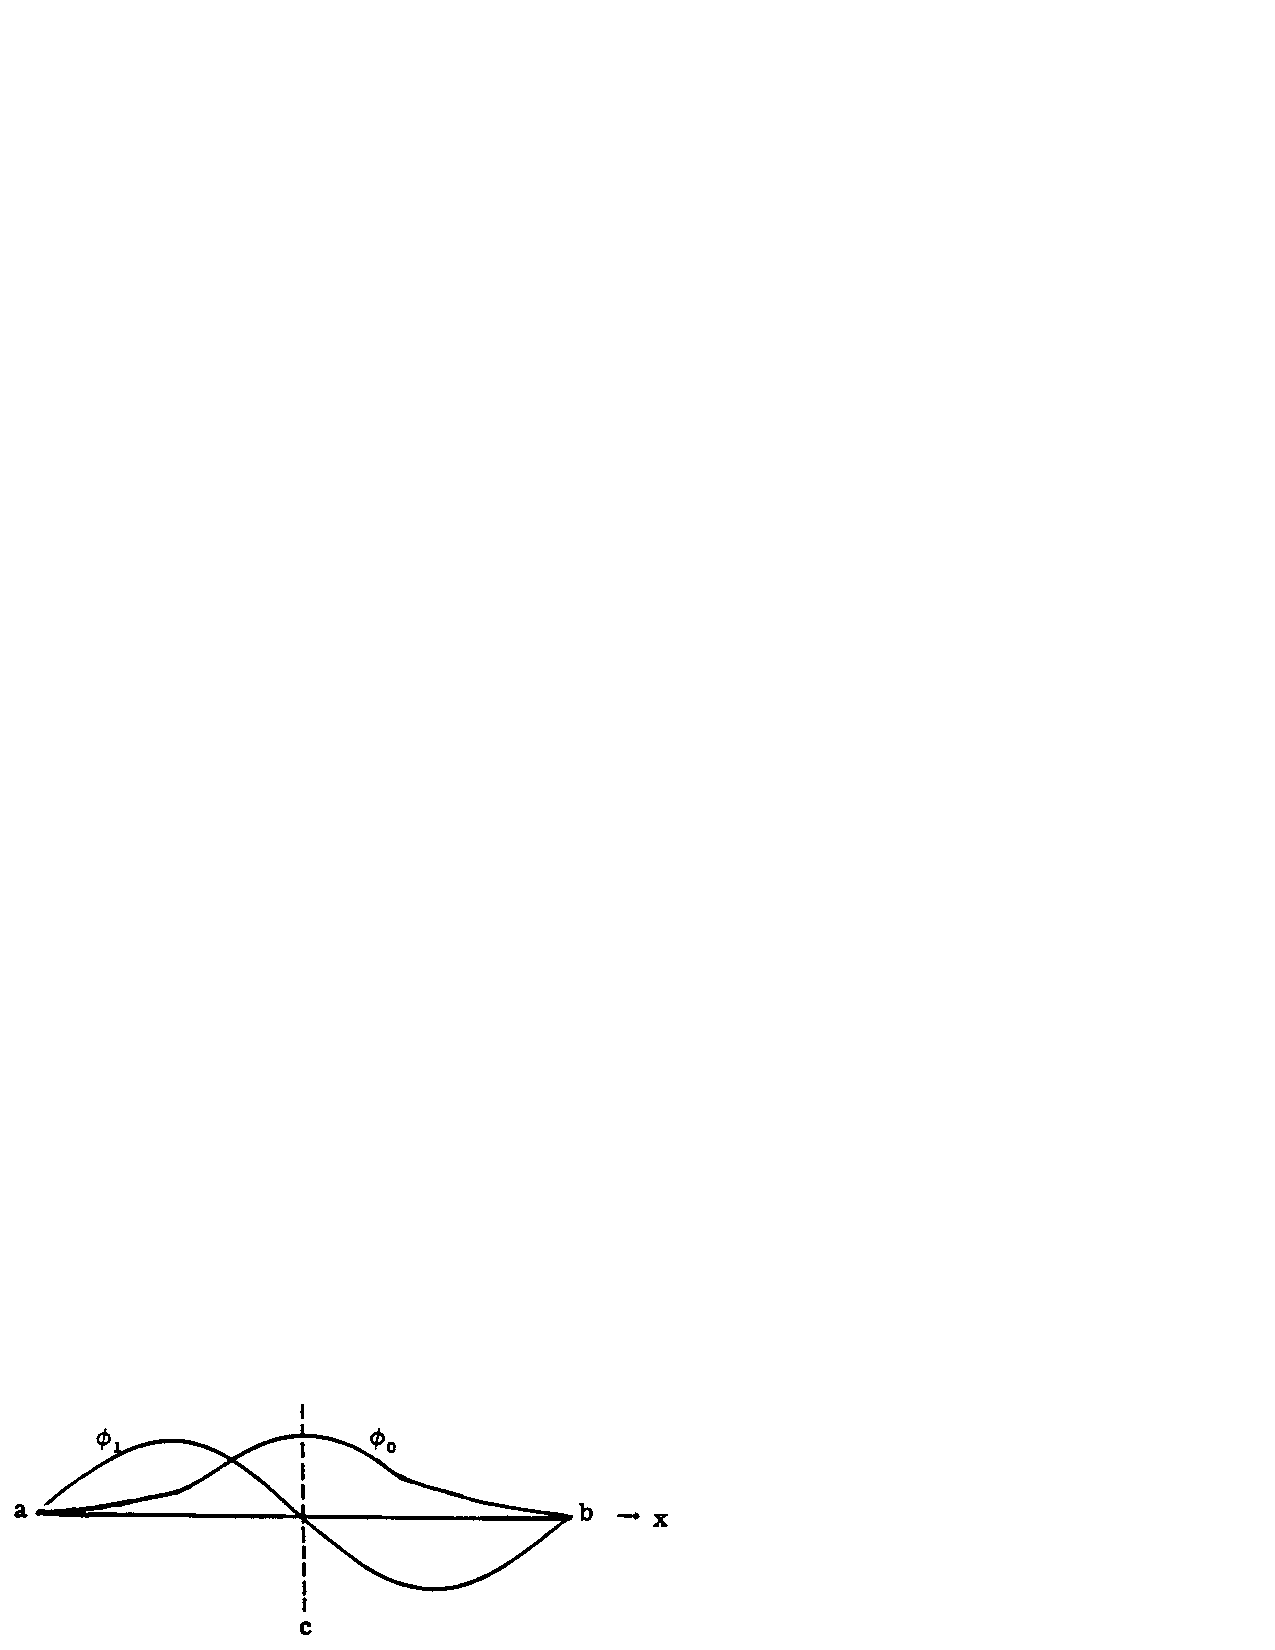
\includegraphics{fig1-20}
\caption{$\varphi_0$ and $\varphi_1$ Nodal Theorem Proof.}
\label{fig1-20}
\end{figure}

First we will show that $E_1 \geq E_0$. Letting $c$ be the location of the node
in $\varphi_1$, we consider the region
\begin{equation}
a < x < c
\label{eqno1app-12}
\end{equation}
so that both $\varphi_0$ and $\varphi_1$ are positive. Then from
equation (\ref{eqno1app-11}) we have
\begin{equation}
E_0 = V + {1 \over \varphi_0} {\hat T} \varphi_0
\end{equation}
and
\begin{equation}
E_1 = V + {1 \over \varphi_1} {\hat T} \varphi_1
\end{equation}
for all points in region (\ref{eqno1app-12}). Thus, the energy
difference is given by
\begin{equation}
E_1 - E_0 = + {1 \over \varphi_1} {\hat T} \varphi_1 - {1 \over 
\varphi_0} {\hat T} \varphi_0 = {1 \over \varphi_1 \varphi_0} \left[ 
\varphi_0 \left( {\hat T} \varphi_1 \right) - \varphi_1 \left( {\hat 
T} \varphi_0 \right) \right].
\label{eqno1app-13}
\end{equation}
The integral over all space of the term in brackets is zero, since $T$ is 
Hermitian,
\begin{equation}
\int^{b}_{a} d x \left[ \varphi_0 \left( {\hat T} \varphi_1 
\right) - \varphi_1 \left( {\hat T} \varphi_0 \right) \right] = \langle 
\varphi_0 \vert {\hat T} \vert \varphi_1 \rangle - \langle {\hat T} \varphi_0 
\vert \varphi_1 \rangle = 0 .
\end{equation}
However, the integrand is generally not zero. For a one-dimensional system, 
the orbitals can always be taken as real.
    
To estimate the sign of equation (\ref{eqno1app-13}), we multiply by
$\varphi_1 \varphi_0$, then integrate from $a$ to $c$, and then divide
appropriately to obtain
\begin{equation}
\left( E_1 - E_0 \right) = {B \over A} ,
\label{eqno1app-14}
\end{equation}
where
\begin{equation}
B = \int^{c}_{a} d x \varphi_0 {\hat T} \varphi_1 -
\int^{c}_{a} d x  \varphi_1 {\hat T} \varphi_0
\label{eqno1app-15}
\end{equation}
and
\begin{equation}
A = \int^{c}_{a} d x \varphi_1 \varphi_0.
\label{eqno1app-16}
\end{equation}
Integrating by parts, the first term of equation (\ref{eqno1app-15})
becomes 
\begin{eqnarray}
\int^c_a dx\ \varphi_0 {\hat T} \varphi_1 
   &=& {1\over 2M}\int^c_a dx\ \varphi_0 
        \left[ {\partial^2 \varphi_1 \over \partial x^2} \right]\cr
   &=& \left\{ + {1 \over 2M} \int^{c}_{a} d x \left[ {\partial 
\varphi_0 \over \partial x} \right] \left[ {\partial \varphi_1 \over 
\partial x} \right] \right\} - \left\{ \left[ {1 \over 2M} \varphi_0 
\left( {\partial \varphi_1 \over \partial x} \right) \right]^c_a 
\right\}\cr
   &=& \left\{ - {1 \over 2M} \int^{c}_{a} d x {\partial^2 
\varphi_0 \over \partial x^2} \varphi_1 \right\} + {1 
\over 2M} \left\{ \left[ \left( {\partial \varphi_0 \over \partial x} 
\right) \varphi_1 - \varphi_0 \left( {\partial \varphi_1 \over 
\partial x} \right) \right]^c_a \right\}.\cr
\label{eqno1app-17}
\end{eqnarray}
Combining equations (\ref{eqno1app-14}) through (\ref{eqno1app-17}),
we obtain
\begin{equation}
\left( E_1 - E_0 \right) = {1 \over 2M} \left[ \varphi_1 \left( 
{\partial \varphi_0 \over \partial x} \right) - \left( {\partial 
\varphi_1 \over \partial x} \right) \varphi_0 \right]^c_a .
\end{equation}
Since $\varphi_1 (c) = 0$, $\varphi_0 (c) > 0$,
\begin{equation}
\left( {\partial \varphi_1 \over \partial x} \right)_{x=c} < 0
\end{equation}
and
\begin{equation}
A = \int_{a}^{c} d x \varphi_1 ^* \varphi_0 > 0,
\end{equation}
we obtain
\begin{equation}
E_1 - E_0 = - {1 \over 2A} \varphi_0 (c) \left( {\partial \varphi_1 
\over \partial x} \right)_{x=c} > 0 ,
\label{eqno1app-18}
\end{equation}
that is,
\begin{equation}
E_1 - E_0 > 0.
\label{eqno1app-19}
\end{equation}
Thus, the nodeless wavefunction has a lower energy than the wavefunction 
with one node. The same proof shows that $\varphi_0$ has a lower energy 
than any wavefunction with more than one node. Hence, the ground state of 
the system has no nodal points, inside the boundaries.
    
Similarly, the above proof can be applied to the comparison of $E_n$ 
and $E_{n+1}$.   That is, the energies for wavefunctions having $n$ and 
$n + 1$ nodes, respectively. The result is that
\begin{equation}
E_{n+1} > E_n ,
\label{eqno1app-20}
\end{equation}
and hence, the eigenstates of a system have energies increasing in the 
same sequence as the number of nodes.

\subsubsection{Singular Potentials}

To obtain equation (\ref{eqno1app-19}) we assumed in equation
(\ref{eqno1app-18}) that
\begin{equation}
\varphi_0 (c) \not= 0
\label{eqno1app-21a}
\end{equation}
and that
\begin{equation}
\left( {\partial \varphi_1 \over \partial x} \right)_{x=c} \not= 0 
.
\label{eqno1app-21b}
\end{equation}
Usually these conditions (\ref{eqno1app-21a})--(\ref{eqno1app-21b})
are satisfied. However, there can be cases where the potential is such
that one of the quantities in
(\ref{eqno1app-21a})--(\ref{eqno1app-21b}) is zero. In this case, we
have $E_1 - E_0 = 0$, and hence, the general condition
(\ref{eqno1app-19}) should be $E_1 \geq E_0$, and (\ref{eqno1app-20})
should be $E_{n+1} \geq E_n$.

For example, consider the case wherein the potential $V(x)$ is so
strongly repulsive at some point $c$, that all solutions of finite
energy must have a node at $c$. In this case, the functions
$\varphi_0$ and $\varphi_1$ in Figure \ref{fig1-20} will have the
shapes in Figure \ref{fig1-21}.
\begin{figure}
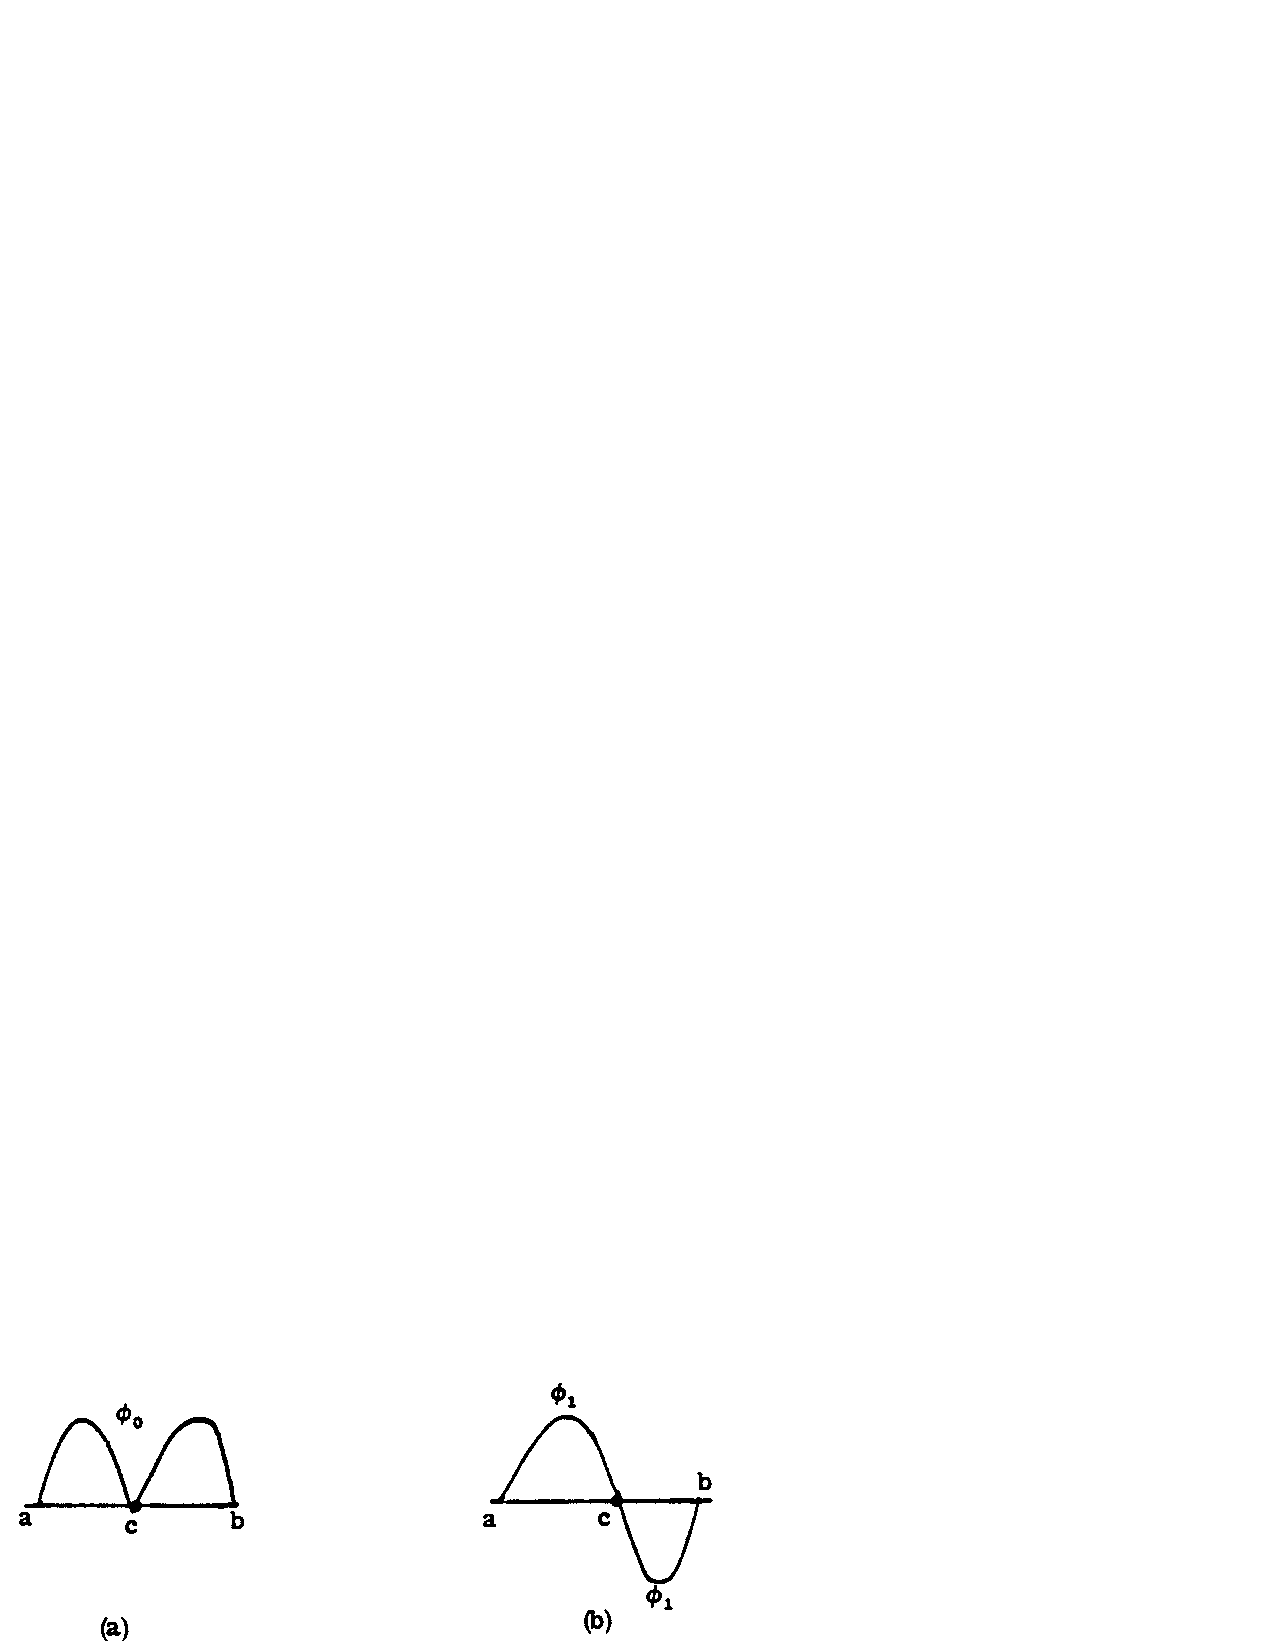
\includegraphics{fig1-21}
\caption{}
\label{fig1-21}
\end{figure}

\noindent
From this figure, the first two solutions for a potential, sufficiently 
singular at point $c$, are shown.
    
From equation (\ref{eqno1app-18}), this leads to$ E_1 = E_0 = 0$, so
that $E_0$ and $E_1$ are degenerate. In this case, the functions
$\varphi_0$ and $\varphi_1$ will have the same shape in each region.
At $x = c$, one of them changes sign but since both must be zero
there, they have the same energy.
    
If the potential is not singular at $c$, the function $\varphi_0$ can 
generally lead to a lower energy by being positive near $c$, thereby 
obtaining a smaller kinetic energy.
    
The presence of cases, such as in Figure \ref{fig1-9}(a), complicated
our notation for the states, in referring to the number of nodes. To
keep things simple, $n$ refers to the number of points at which the
wavefunction changes sign.
    
Singularities in the potential would also lead to equalities in the energies for some
excited states, $E_{n+1} = E_n$.

\subsubsection{A Singular Example}
    
As discussed above, the equal sign in (\ref{eqno1app-9}) would occur
when the potential $V(x)$ is sufficiently singular, that the best
non-negative wavefunction $\varphi_0$ has a node at some point.  For
example, if
\begin{equation}
V ( x ) = {1 \over \vert x - x_0 \vert},
\end{equation}
the potential energy is
\begin{equation}
\langle \varphi (x) \vert V ( x ) \vert \varphi ( x ) \rangle = 
\int^{x_0}_{- \infty} d x {\vert \varphi ( x ) \vert^2 \over 
\vert x - x_0 \vert} + \int^{\infty}_{x_0} d x 
{\vert \varphi ( x ) \vert^2 \over 
\vert x - x_0 \vert} .
\end{equation}
Expanding 
\begin{equation}
\varphi (x) = \varphi (x_0) + ( x - x_0 ) \varphi^{\prime}(x_0) + \cdots
\end{equation}
we see that the dominant term in the integral
\begin{equation}
\int^{x_0}_\infty dx {\varphi (x)^2 \over \vert x - x_0 \vert} 
\end{equation}
is
\begin{equation}
\varphi \left( x_0 \right)^2 \int^{x_0}_\infty {dx \over ( x - 
x_0)} = \varphi \left( x_0 \right)^2 \ln 0
\end{equation}
and hence, the energy diverges if $\varphi ( x_0 ) \not= 0$.

Thus, for $\varphi$ to yield an $E < \infty$, and hence to describe
the ground state, it must be that $\varphi (x) \rightarrow 0$ as $x
\rightarrow 0$.  In this case, $E_0 = E_1$, assuming no other
singularities in $V(x)$.

\subsection{The Ground State of Hydrogen Atom}
\label{app-d}
    
In summary, the ground state of the hydrogen-like atom, with nuclear 
charge $Z$, has the wavefunction
\begin{equation}
\psi ( r , \nu , \varphi ) = N_0 e^{-{Zr \over a_0}} ,
\end{equation}
where
\begin{equation}
N_0  = \sqrt{{Z^3 \over \pi a^3_0}}
\end{equation}  
and
\begin{equation}
a_0 = {\hbar \over me^2}
\end{equation}  
is defined as the Bohr. The energy of this wavefunction is
\begin{equation}
E = - {1 \over 2} Z^2 \left[ {e^2 \over a_0} \right] = - {1 \over 2} 
{Ze^2 \over {\bar R}} ,
\end{equation}
where
\begin{equation}
{\bar R} = {a_0 \over A}
\end{equation}
is the average size of the atom, and $a_0$ is denoted as the Bohr radius.

\subsubsection{Solution of the Schr\"odinger Equation}
    
We will solve, for the ground state of the hydrogen atom, that is, the 
lowest solution of
\begin{equation}
\left[ - {\hbar^2 \over 2m} \nabla^2 - {Ze^2 \over r} \right] \psi ( 
r , \theta , \varphi ) = E \psi ( r , \theta , \varphi ).
\label{eqno1app-22}
\end{equation}
Since the potential term is independent of angle, the wavefunction has
the form
\begin{equation}
\psi ( r , \theta \varphi ) = f ( r ) Z ( \theta , \varphi ) ,
\end{equation}
where the angular function $Z( \theta, \varphi)$ is a constant for the
ground state,
\begin{equation}
Z ( \theta , \varphi ) = {1 \over \sqrt{4 \pi}}.
\label{eqno1app-23}
\end{equation}
The normalization condition is
\begin{equation}
\int^{2 \pi}_{0} d \varphi \int^{\pi}_{0} \sin \theta d 
\theta \left[ Z \left( \theta , \varphi \right) \right]^2 = 1,
\end{equation}
leading to equation (\ref{eqno1app-23}). Thus, our chore is to solve
\begin{equation}
- {\hbar^2 \over 2m} \nabla^2 f ( r ) - {Ze^2 \over r} f ( r ) 
= E f ( r ).
\label{eqno1app-24}
\end{equation}
First we must express $\nabla^2 f ( r )$ in terms of spherical 
coordinates.
\begin{equation}
z = r \cos \theta,
\end{equation}
\begin{equation}
x = r \sin \theta \cos \theta,
\end{equation}
\begin{equation}
y = r \sin \theta \sin \varphi,
\end{equation} 
and 
\begin{equation}
r^2 = x^2 + y^2 + z^2.
\end{equation}
Since
\begin{equation}
\left[ {\partial r \over \partial z} \right]_{x,y} = {\partial \over 
\partial z} \sqrt{x^2 + y^2 + z^2} = {z \over r}
\end{equation}
where the subscript $x,y$ indicates that $x$ and $y$ are fixed, we 
see that
\begin{equation}
\left[ {\partial \over \partial z} f ( r ) \right]_{x,y} = \left[ 
{\partial r \over \partial z} \right]_{x,y} \left[ {\partial f \over 
\partial r} \right] = {z \over r} f^\prime( r ) .
\end{equation}
Thus, letting
\begin{equation}
f^{\prime \prime} ( r ) = {d^2 f \over dr^2}
\end{equation}
and
\begin{equation}
f^\prime( r ) = {d f \over dr} ,
\end{equation}
we obtain
\begin{eqnarray}
{\partial^2 \over \partial z^2} f(r) = {\partial \over \partial z} 
\left[ {z \over r} f^{\prime} (r) \right] &=& {1 \over r} f^{\prime} 
(r) + z {\partial x \over \partial r} {\partial \over \partial r} 
\left[ {1 \over r} f^{\prime} (r) \right]\cr
&=& {1 \over r} f^{\prime} (r) + {z^2 \over r} \left[ {1 \over r} 
f^{\prime \prime} (r) - {1 \over r^2} f^{\prime} (r) \right]\cr
&=& \left[ {1 \over r} - {z^2 \over r^3} \right] 
f^{\prime} (r) + {z^2 \over r^2} f^{\prime \prime} (r).
\end{eqnarray}
Combining with $\partial^2 / \partial x^2 f(r)$ and $\partial^2 / 
\partial y^2f(r)$ leads, then, to
\begin{equation}
\nabla^2 f ( r ) = f^{\prime \prime} (r) + {2 \over f} f^{\prime}(r)
\label{eqno1app-25}
\end{equation}
Substituting equation (\ref{eqno1app-25}) into equation
(\ref{eqno1app-24}), leads to
\begin{equation}
- {\hbar^2 \over 2m} \left[ {d^2f \over dr^2} + {2 \over r} {df \over 
df} \right] - {Ze^2 \over r} f ( r ) = E f (r)
\label{eqno1app-26}
\end{equation}
as the Schr\"odinger equation.  Since the potential in equation
(\ref{eqno1app-22}) goes to zero as $r \rightarrow \infty$, only the
state with $E < 0$ are bound, and hence we take $E < 0$.  Consider now
a sufficiently larger $r$ that
\begin{equation}
\vert {Ze^2 \over r} \vert \ll \vert E \vert
\end{equation}
and
\begin{equation}
{2 \over r} \vert {df \over dr} \vert \ll \vert {d^2f \over dr^2} \vert .
\end{equation}
In this case, equation (\ref{eqno1app-26}) reduces to
\begin{equation}
{d^2 f \over \partial r^2} = \zeta^2 f(r),
\label{eqno1app-27}
\end{equation}
where
\begin{equation}
\zeta^2 = - {2mE \over \hbar^2} \geq 0.
\label{eqno1app-28}
\end{equation}
The solution of equation (\ref{eqno1app-27}) is
\begin{equation}
f(r) = e^{- \zeta r} .
\label{eqno1app-29}
\end{equation}
Thus, all bound state solutions of equation (\ref{eqno1app-28}) must
necessarily go to zero exponentially. Note that in the limit of very
large $r$, the function $r^n e^{-\zeta r}$ would also satisfy equation
(\ref{eqno1app-26}).

Consider now the substitution of the exponential function
(\ref{eqno1app-29}) into the Schr\"odinger equation (\ref{eqno1app-26}),
\begin{equation}
{d^2 f \over \partial r^2} + {2 \over r} {df \over dr} - \zeta^2 f(r) 
= - {2mZe^2 \over \hbar^2} {1 \over r} f(r).
\end{equation}
From equation (\ref{eqno1app-27}) the first term of each side, the
long-range terms, cancel at all $r$ leaving
\begin{equation}
{2 \over r} {df \over dr} = - {2 \zeta \over r} f(r) = - {2mZe^2 
\over \hbar^2} {1 \over r} f(r).
\end{equation}
Thus, the exponential function (\ref{eqno1app-29}) is an eigenfunction of the Schr\'odinger
equation if
\begin{equation}
\zeta = {mZe^2 \over \hbar^2}.
\end{equation}
Since $\zeta$ has the units of inverse length, e.g., see equation
(\ref{eqno1app-28}), it is convenient to consider the length quantity
$a_0 = \hbar / me^2$, referred to as the Bohr radius or simply the
Bohr, as the fundamental atomic length leading to $\zeta = Z/a_0$.
From equation (\ref{eqno1app-27}) the value of $\zeta$ is related also
to the energy,
\begin{equation}
E = - {\hbar^2 \over 2m} \zeta^2.
\end{equation}
Thus,
\begin{equation}
E = - \left[ {\hbar^2 \over 2m} \right] {Z^2 \over a^2_0} = - {1 \over 
2} Z^2 \left[ {e^2 \over a_0} \right].
\end{equation}

Summarizing, we find that the wavefunction
\begin{equation}
\psi_0 ( r , \theta , \varphi ) = f ( r ) = N_0 e^{-{Zr \over 
a_0}},
\label{eqno1app-30}
\end{equation}
is an eigenfunction of the Schr\"odinger equation with an energy of
\begin{equation}
E_0 = - {1 \over 2} Z^2 \left[ {e^2 \over a_0} \right],
\end{equation}
where $a_0 - \hbar^2 / m e^2$.  Since the wavefunction
(\ref{eqno1app-30}) is nodeless, we know from the nodal theorem that
this eigenfunction of ${\hat H}$ is the ground state of the hydrogen
atom. For the wavefunction (\ref{eqno1app-30}), the average value of
$1/r$ is
\begin{equation}
{1 \over {\bar H}} = \langle \psi \vert {1 \over r} \vert \psi 
\rangle = {Z \over a_0}.
\end{equation}
Thus, the average potential energy is
\begin{equation}
{\bar V} = \langle \psi \vert - {Ze^2 \over r} \vert \psi \rangle = - 
{Ze^2 \over r} = - {Z^2e^2 \over a_0}
\end{equation}
and the total energy can be written as
\begin{equation}
E = {1 \over 2} {\bar V} = - {1 \over 2} {Ze^2 \over {\bar R}} = - {1 
\over 2} {Z^2e^2 \over a_0}.
\end{equation}

In order to normalize the wavefunction (\ref{eqno1app-30}), note that
\begin{equation}
\langle \psi \vert \psi \rangle = \int^{\infty}_{0} r^2 dr 
\int^{\pi}_{0} \sin \theta d \theta \int^{2 \pi}_{0} d 
\varphi \left[ f ( r ) \right]^2 = 4 \pi \int^{\infty}_{z} r^2 
drf(r)^2,
\end{equation}
where the angular integral is
\begin{equation}
\int d \Omega = \int^{\pi}_{0} \sin \theta d\theta \int^{2 
\pi}_{0} d\varphi = 4 \pi.
\end{equation}
Since
\begin{equation}
\int^{\infty}_{0} r^2 drf(r)^2 = N_0^2 \int^{\infty}_{0} 
r^2 dre^{-2 \zeta r} = {N_0^2 \over (2 \zeta)^3} 
\int^{\infty}_{0} \rho^2 d \rho e^{- \rho} = {N_0^2 \over (2 
\zeta)^3} 2!,
\end{equation}
we see that
\begin{equation}
N_0 = \sqrt{{\zeta^3 \over \pi}} = \sqrt{{Z^3 \over \pi a^3_0}}.
\end{equation}

\subsubsection{Analysis of the Wavefunction}
    
A plot of the orbital along the $z$ axis is given in Figure
\ref{fig1-22}.  Note that the slope of the wavefunction is
discontinuous at $z = 0$. This singular behavior is referred to as a
cusp and results from the singular behavior in the potential energy at
this point.
\begin{figure}
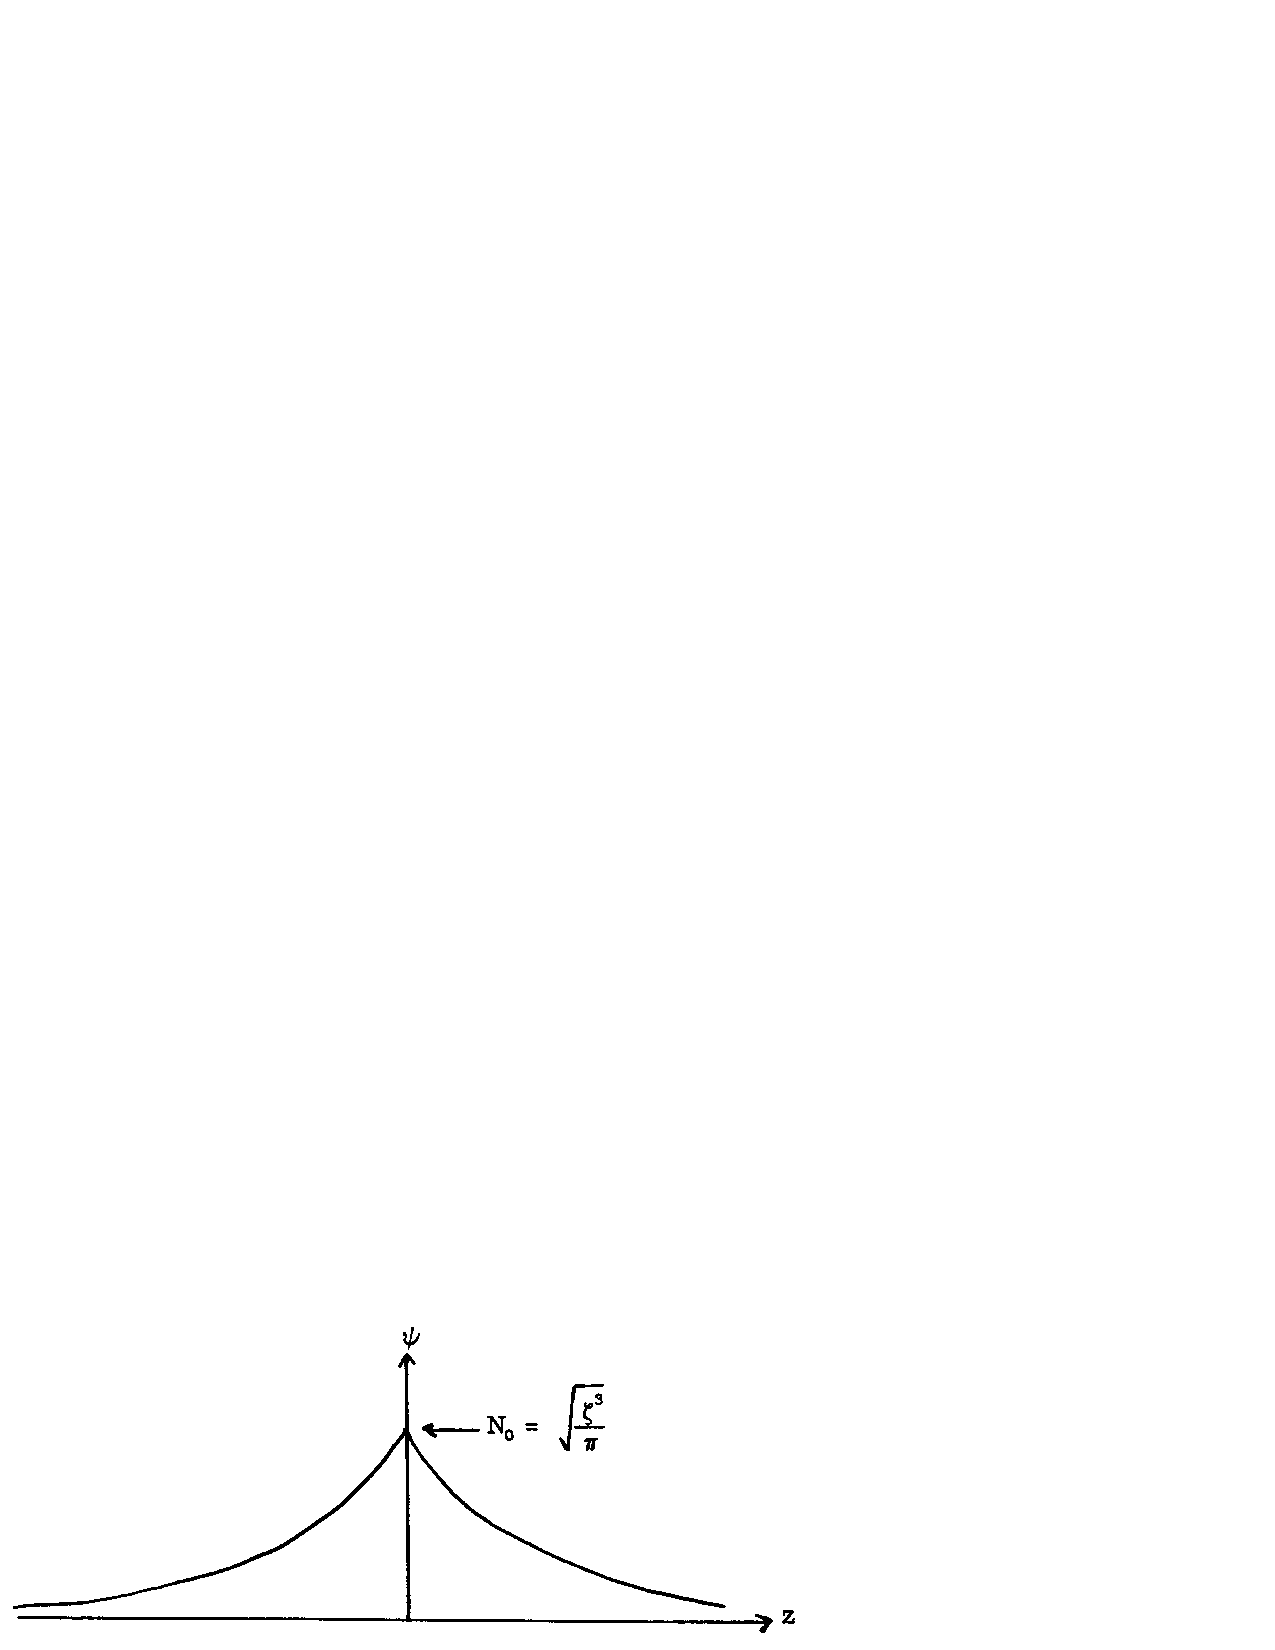
\includegraphics{fig1-22}
\caption{}
\label{fig1-22}
\end{figure}

\noindent
In Figure \ref{fig1-22}, the ground state wavefunction, $\psi_0$, for
the $H$ atom, plotted along the $z$ axis, is illustrated.
    
The Schr\"odinger equation (\ref{eqno1app-23}) says that $Ef (r)$ is equal to
\begin{equation}
- {\hbar^2 \over 2m} \nabla^2 f(r) - {Ze^2 \over r} f(r)
\end{equation}
for every point $r$. But, as $r \rightarrow 0$, the term
\begin{equation}
- {Ze^2 \over r} f(r)
\end{equation}
goes to $- \infty$. Thus, since $Ef (r)$ is finite, the Schr\"odinger 
equation requires that
\begin{equation}
- {\hbar^2 \over 2m} \nabla^2 f(r)
\end{equation}
goes to $+ \infty$ as $r \rightarrow 0$. The cusp in the wavefunction leads 
to a $\nabla^2 f (r)$ that goes to $+ \infty$ as $r \rightarrow 0$
and exactly cancels the negative singularity in the potential term.

\subsection{Rydberg Atomic Units}
\label{app-e}
    
Another set of atomic units used occasionally, employs as the unit of energy the
ionization potential of the hydrogen atom,
\begin{equation}
R_{\infty} = {me^4 \over 2 \hbar^2}.
\end{equation}
This quantity is called the Rydberg and is related to the Hartree by one 
Rydberg equal to one-half Hartree. With this choice for the unit of 
energy, $me^4 /2 \hbar^2 = 1$, we cannot use the convenient sets of units 
in the text. If the unit of length is still taken as the Bohr, 
$\hbar^2 /me^2 = 1$, then Rydberg units led to $me^4 = 2 \hbar^2
= 2me^2$, and hence we must choose $|e| = \sqrt{2}$ and $\hbar^2 = 2m$. If 
we taken $m = 1$, then $\hbar = \sqrt{2}$. These units are sometimes used
by scattering theorists since the kinetic energy of a plane wave, 
$(\hbar^2/2m)/k^2$ simply becomes $k^2$. Also, some workers reporting 
band calculations on solids use Rydberg units. The series of books by Slater 
also used these units. However, the regular atomic units, or Hartree atomic 
units, as described in the text, axe more convenient and more common, and 
we will always use them.

\subsection{Units and Conversion Factors}
\label{app-f}
    
\subsubsection{International System of Units}
    
In an effort to bring some order to the proliferation of units that 
continues to occur in the sciences, an international group in 1960, adopted what
is referred to as the International System of Units, or may be called SI units.
    
In this system, there are seven fundamental units:

\begin{tabular}{ccc} \\ \hline
Unit & Abbreviation & Physical Quantity\cr
\noalign{\medskip\hrule\medskip}
meter & m & length\cr
kilogram & kg & mass\cr
second & s or sec & time\cr
ampere$^*$ & A & electric current\cr
kelvin$^*$ & K & terhmodynamic temprature\cr
mole & mol & amount of substance\cr
candela & cd & luminous intensity\cr
\hline
\end{tabular}\\
\noindent$^*$Note that some units are not capitalized even though they
are derived from the names of people.

From these fundamental units can be derived a number of combined units
that prove quite useful. Thus, from Newton's Law, $F = ma$, we know
that force has units of
\begin{equation}
{\mathrm{mass} \times \mathrm{length} \over \mathrm{time}^2},
\end{equation}
and it is convenient to define the unit of force, Newton's , as one Newton
equal to 1 kg m sec$^{-2}$.  Similarly, a constant force $F$ exerted over a distance
$\ell$ does an amount of work $W$, so that the unit of energy, joule, is one joule
equal to one newton meter equal to one kg m$^2$ sec$^{-2}$.
    
Some commonly derived units, in the International System of Units, are:

\begin{tabular}{cccccc}\\ \hline
Unit & Abbreviation & Definition in Fundamental & Physical Quantity\cr
& & Unit Terms\cr
\noalign{\medskip\hrule\medskip}
liter & $\ell$ & 10$^{-3}m^3$ & volume\cr
newton & N & mkgsec$^{-2}$ & force\cr
joule & J & $Nm=m^2$ kgsec$^{-2}$ & energy\cr
watt & W & Jsec$^{-1}=m^2$ kgsec$^{-2}$ & power\cr
pascal & Pa & $Nm^{-2}=m^{-1}$ kgsec$^{-2}$ & pressure\cr
coulomb & C & A sec & electric charge\cr
volt & V & $WA^{-1}=m^2$ kgsec$^{-2}$A$^{-1}$ & electric potential\cr
ohm & $\Omega$ & $VA^{-1}=m^2$ kgsec$^{-3}$A$^{-2}$&electri 
resistance\cr
hertz & Hz & sec$^{-1}$ & frequency\cr
\hline
\end{tabular}

The acceptable multiples, or fractions, to be used for the basic 
International Systems of Units are designed by the following prefixes:
    
\begin{tabular}{ccc}\\ \hline
Fraction & Prefix & Symbol Quantity\cr
\noalign{\medskip\hrule\medskip}
10$^{-18}$ & atto & a\cr
10$^{-15}$ & femto & f\cr
10$^{-12}$ & pico & p\cr
10$^{-9}$ & nano & n\cr
10$^{-6}$ & micro $\mu$\cr
10$^{-3}$ & milli & m\cr
10$^{-2}$ & centi & c\cr
10$^{-1}$ & deci & d\cr
10 & deka & da\cr
10$^2$ & hecxto & h\cr
10$^3$ & kilo & k\cr
10$^6$ & mega & M\cr
10$^9$ & giga & G\cr
10$^{12}$ & tera & T\cr
\hline
\end{tabular}
    
Although, the above fundamental units are convenient for a number of 
quantities, they are quite inconvenient for others. Some examples include:
    
\begin{tabular}{ccc} \\ \hline
Physical Quantity & Abbreviation & Definition in SI Units\cr
Charge on an Electron & e & 1.602189 $\times 10^{-19}$ C\cr
Atmospheric Pressure & atm & 101.325 Pa\cr
\hline
\end{tabular}
    
For the atmospheric pressure, this is at sea level.
    
Other units are not necessarily superior to the International System of Unit 
quantities, but their use is so widespread that scientists must be facile 
with their use. Some examples include:

\begin{enumerate}    
\item Kilocalorie, the original definition was the energy to heat 
1 kg of H$_2$0 by a temperature of $1^{\circ}$K, at 15$^{\circ}$C. Abbreviated 
as kcal, and its relation to fundamental units is I kcal = 4.18 kJ, defined 
to be exact.
    
\item Angstrom, abbreviated as \AA, and its relation to fundamental units is
1 \AA = 10$^{-10}m = 10^{-3}$ cm.
    
\item Electron volt, defined as the energy change upon moving a charge of
one electron through an electric potential of one volt. Abbreviated as
eV, and its relations to fundamental units as 1 eV = 96.483 kJ 
mol$^{-1}$.

\end{enumerate}

\subsubsection{Units for Coulomb's Law}
    
Conversion between units can sometimes get confusing for coulomb 
interactions.  Coulomb law states that the force between two charges 
$Q_1$ and $Q_2$, separated by a distance $R$ is
\begin{equation}
F_{tot} = {Q_1 Q_2 \over R^2}
\end{equation}
where $F_{tot}$ is the total force. Hence, the energy of interaction
is
\begin{equation}
E = \int^{R}_{- \infty} F \cdot d r = {Q_1Q_2 \over R}.
\end{equation}

In cgs units, we define the electrostatic unit of charge, esu, as that 
charge which leads to a force of one dyne when the charges are separated 
by one cm. Thus,
\begin{equation}
\mathrm{Force}(\mathrm{dynes}) = {[Q(\mathrm{esu})]^2 
       \over [R(\mathrm{cm})]^2}
\end{equation}
and
\begin{equation}
\mathrm{Energy}(\mathrm{ergs}) = {[Q(\mathrm{esu})]^2 
        \over R(\mathrm{cm})}.
\end{equation}
    
In the International System of Units, the unit of charge, the Coulomb, is 
defined in terms of a current, one ampere is equal to one Coulomb/sec. Also 
the units of current are related to force and distance through a different 
force law, magnetic induction. The relation between Coulombs and esu, turns 
out to be
\begin{equation}    
1\ \mathrm{Coulomb} = {1\ \mathrm{esu} \over (2.99810^9)},
\end{equation}
where the 2.998 comes from the speed of light, 2.998 10$^8$ m/sec. Since
\begin{equation}
\mathrm{Force}(\mathrm{newtons}) = 10^{-5}\mathrm{Force}(\mathrm{dynes})
\end{equation}
and
\begin{equation}
R(\mathrm{meters}) = 10^{-2} R(\mathrm{cm}), 
\end{equation}   
the Coulomb law becomes
\begin{equation}    
\mathrm{Force}(\mathrm{newtons}) = [8.98810^9] 
       {[Q(\mathrm{Coulomb})]^2 \over [R(\mathrm{m})]^2}
\end{equation}
and
\begin{equation}
\mathrm{Energy}(\mathrm{joules}) = [8.98810^9] 
         {[Q(\mathrm{Coulomb})]^2 \over [R(\mathrm{cm})]}.
\end{equation}
In SI units, the constant in this expression is generally written as
\begin{equation}   
8.988 \times 10^9 = {1 \over 4 \pi \epsilon_0},
\end{equation}
where
\begin{equation}
\epsilon_0 = 8.85410^{-12}\ \mathrm{C}^2\mathrm{N}^{-1}\mathrm{m}^{-2}
\end{equation}
is called the \emph{permittivity of a vacuum}. This leads to
\begin{equation}
\mathrm{Energy}(\mathrm{N}) = {Q_1(\mathrm{C})Q_2(\mathrm{C})
        \over 4 \pi \epsilon_0 R(\mathrm{m})}
\end{equation}
for the Coulomb energy.
    
In this case, the $Q_1$ and $Q_2$ are always some multiple of the fundamental 
charge on a proton, or electron,
\begin{equation}
1\ e = 1.60210^{-19}\ \mathrm{C}
\end{equation}
and
\begin{equation}
1\ e = 4.80310^{-10}\ \mathrm{esu}.
\end{equation}
Thus, we will write
\begin{equation}
Q_1 = q_1\ e
\label{eqno1app-31a}
\end{equation}
\begin{equation}
Q_2 = q_2\ e
\label{eqno1app-31b}
\end{equation}
where $q_1$ and $q_2$ have no units. In addition, we will often 
write $R$ in terms of Bohr radii, for example,
\begin{equation}
R = r\ a_0,
\label{eqno1app-32}
\end{equation}
where $r$ has no units. In this case, the Coulomb energy becomes
\begin{equation}
E = {q_1q_2 \over r} \left[ {e^2 \over a_0} \right]
\label{eqno1app-33}
\end{equation}
where no $4 \pi \epsilon_0$ factor is included. In equation
(\ref{eqno1app-33}), the unit of energy is
\begin{equation}
1\ h_0 = 1\ hartree = {e^2 \over a_0}
\label{eqno1app-34a}
\end{equation}
and
\begin{equation}
1\ h_0 = 27.2116\ \mathrm{eV} = 2625.5\ \mathrm{kJ}/\mathrm{mol} 
         = 627.51\ \mathrm{kcal}/\mathrm{mol}.
\label{eqno1app-34b}
\end{equation}
The fast way to calculate atomic level Coulomb energies, in various
units, is to first express all distances and charges in atomic
units. As in equations (\ref{eqno1app-31a})--(\ref{eqno1app-31b}) and
(\ref{eqno1app-32}), calculate the energy using (\ref{eqno1app-33})
and then to convert from atomic units to SI units using equations
(\ref{eqno1app-34a}) --(\ref{eqno1app-34b}).
    
For example, calculate the interaction of two protons at a distance 
of $R = 5$ \AA. The answer is
\begin{equation}
R = 5\ \mathrm{\AA} = {5 \over 0.529}\ a_0 = 9.45\ a_0
\end{equation}
\begin{equation}
E(h_0) = {1 \over R(a_0)} = {1 \over 9.45} = 0.1058\ h_0
\end{equation}
both equal to 2.88 eV = 278 kJ/mole = 66.4 kcal/mol.
    
Useful conversion factors here, are
\begin{equation}
e^2 = 14.3998eV\ \mathrm{\AA} = 332.059\ (\mathrm{kcal}/\mathrm{mol})\mathrm{\AA}.
\end{equation}

\subsubsection{Units for Mass}
    
In atomic units, the mass of the electron is unity. However, this is
not to be confused with the atomic mass unit, amu, which is the
standard for relating the masses of atoms. The modern convention is to
define the dominant isotope of C, i.e., $^{12}$C, as having a mass of
12.0000. In these units, the mass of the hydrogen atom is 1.00783 amu,
the mass of a proton is 1.00728 amu, and the mass of an electron is
1/18.22.89 amu. Thus, in atomic units, hartree, the mass of the proton
is
\begin{equation}
1.00728 \times 1822.89 = 1836.16.
\end{equation}
The conversion to SI units is
\begin{equation}
1\ \mathrm{amu} = 1.660566 \times 10^{-27}\ \mathrm{kg}.
\end{equation}

\subsubsection{Energy Quantities for Photons}
    
The wavelength, $\lambda$, and frequency, $\nu$, of light are related by the 
speed of light, $c$, $\lambda \nu = c$.  Thus, since 2 = 2.99792458 
$\times$ 10$^{10}$ cm/sec, the frequency for yellow light, 
$\lambda =$ 600 nm, is
\begin{equation}
\nu = {3 \times 10^{10} \over 6 \times 10^{-7}} = 5 \times 10^{16} 
\mathrm{Hz}
\end{equation}
where one Hz is equal to one cycle per second, and the wavelength for KZLA, 
$\nu =$ 94 MHz, is
\begin{equation}
\lambda = {3 \times 10^{10} \over 94 \times 10^6} = 319\ \mathrm{cm} =
3.19\ \mathrm{m}.
\end{equation}

In the quantum description of light, the energy of a photon is given
by $E = h \nu$, where $h = 2 \pi \hbar$ is the original Planck's
constant. Thus, the energy of a photon of light can be expressed as
\begin{equation}
E = h \nu = {hc \over \lambda} = hc {\bar \nu}
\end{equation}
where ${\bar \nu} = 1 / \lambda$ is called the wavenumber, and denoted 
as cm$^{-1}$. Substitution for the known values of $h$ and $c$ leads to
\begin{equation}
E(eV) = {1239.85 \over \lambda] (\mathrm{nm})} = 8065.480 {\bar \nu}\
(\mathrm{cm}^{-1})
\end{equation}
and
\begin{equation}
{\bar \nu} ( \mathrm{cm}^{-1}) = {10^7 \over \lambda (\mathrm{nm})}
\end{equation}
Thus, when an electron decreases its energy of 1 eV, dropping into a lower
energy state, it may emit this energy as a single photon with wavelength
$\lambda =$ 1240 nm = 1.24 microns, or wavenumber ${\bar \nu} =$ 
8065 cm$^{-1}$.

\subsubsection{Other Energy Relations}
    
Chemists often use the energy quantity kilocalories per mole, which we will
abbreviate as kcal, 1 eV = 23.06036(14) kcal. Recently, emphasis has been 
placed on SI units in which the kilojoule per mole, denoted as kJpm, is the 
energy unit, 1 kcal = 4.18400 kJpm.
    
The atomic unit of energy, the hartree, is kind of large for convenient use 
and we will often use the millihartree, denoted as mh. Relations between 
these units are
\begin{equation}
1\ \mathrm{eV} = 36.7490\ \mathrm{mh} 
  = 23.0604\ \mathrm{kcal} = 96.4847\ \mathrm{kJpm} 
  = 8065.48\ \mathrm{cm}^{-1},
\end{equation}
and
\begin{equation}
1\ \mathrm{mh} = 0.27212\ \mathrm{eV} = 0.627511\ \mathrm{kcal} 
   = 2.62550\ \mathrm{kJpm} = 219.475\ \mathrm{cm}^{-1}.
\end{equation}
The average thermal energy of an oscillator, at room temperature, is
\begin{equation}
kT = {1 \over 40}\mathrm{eV} = 1\ \mathrm{mh} = 0.6\ \mathrm{kcal} 
   = 200\ \mathrm{cm}^{-1} = 2.4\ \mathrm{kJpm}.
\end{equation}
The strength of the H$_2^+$ bond is
\begin{equation}
2.5\ \mathrm{eV} = 92\ \mathrm{mh} = 58\ \mathrm{kcal} = 24l\ \mathrm{kJpm}.
\end{equation}
The vibrational energy $\hbar \omega_e$ of H$_2^+$ is
\begin{equation}
3000\ \mathrm{cm}^{-1} = 14\ \mathrm{mh} = 8.6\ \mathrm{kcal} 
   = 0.37\ \mathrm{eV} = 36\ \mathrm{kJpm}.
\end{equation}

\subsubsection{Examples}
    
The fundamental constants are experimentally determined and, hence,
the best values for them change with time. For aid in calculating
these constants in the future, we summarize the procedure
\begin{eqnarray}
1 \left( {\mathrm{eV} \over \mathrm{atom}} \right) 
   &&\times 1.60218921 \times 10^{-22} 
   \left({\mathrm{kJ} \over \mathrm{eV}}\right) 
   \times {1 \mathrm{kcal} \over 4.184\mathrm{kJ}}
   \times 6.022045\times 10^{23} \left( {atoms \over mol} \right) \cr
   && = 23.06036\ \mathrm{kcal}/\mathrm{mol}.
\end{eqnarray}
Therefore,
\begin{equation}
1\ {\mathrm{eV} \over \mathrm{atom}} = 23.06036\ \mathrm{kcal}/\mathrm{mol}.
\end{equation}
For force constants, we use the following
\begin{equation}
k = M \omega^2 = {\mathrm{mass} \over \mathrm{time}^2} 
    = {\mathrm{Energy} \over \mathrm{length}^2}
\end{equation}
\begin{eqnarray}
1 au = {h \over a_0^2} &= {27.21161 \times 1.6021892 \times 10^{-12}\
  \mathrm{erg} \over (0.52917706 \times 10^{-8}\ \mathrm{cm})^2}\cr
&= 1.556919 \times 10^6 {\mathrm{dyne} \over \mathrm{cm}}\cr
&= 15.56919 {\mathrm{mdyne} \over \mathrm{A}}.\cr
\end{eqnarray}

\subsubsection{Conversion Factors}
    
Included herein, are the fundamental constants as of 1973
\cite{cohen_taylor}. Commonly used constants are as follows. A number
in parentheses indicates the standard deviation in the error for the
last quoted digit.

\begin{enumerate}
\item 1 bohr = 0.5291771(4) \AA. 

\item 1 hartree = 27.21161(7) eV.
    
\item 1 hartree = 627.5096(4) kcal/mol = 219474.7 cm$^{-1}$. 

\item 1 eV = 23.06036(14) kcal/mol = 96.483 kJ/mol.
    
\item 1 eV = 8065.48(2) cm$^{-1}$.

\item 1 eV = 1239.852(3)/$\lambda$(nm).
    
\item 1 kcal 4.18400 kJ = 349.755 cm$^{-1}$.
    
\item 1 amu 1822.887(l) $m_e$ for atomic masses. This is used to convert 
atomic masses to hartree atomic units, mass $^{12}$C = 12.000.
    
\item 1 au = 15.56919 mdyne/\AA\ for force constant.
    
\item For gas constant, R = 98719(7) cal mol$^{-1}$K$^{-1}$, and 
R = 82.0568 cc atm mol$^{-1}$K$^{-1}$.

\item Avogadro's constant = 6.022045(31 )$\times$10$^{23}$ molecules/mol.

\item $1 / \alpha = \hbar c /e^2$ = 137.03604(11) for fine structure constant.

\item For dipole moment, 1 au = 2.541765(8) Debye, and 1 au
2.541765(8) $\times$ (10$^{-18}$ esu $\times$ cm).

\item For quadrupole moment, 1 au 1.345044 $\times$ 10$^{-26}$ esu
cm$^2$ , and 1 au = 1.345044 Buckingham.

\item 1 au = 3.241391 $\times$ 1015 esu cm$^{-3}$ for electric field gradient.

\item For Coulomb energies, $e^2 / R$ (eV) = 14.3998/R(\AA), and 
$e^2 / R$ (kcal) 332.059/R(\AA).
\end{enumerate}